%\documentclass[onecolumn]{IEEEtranTIE}
%\documentclass[journal]{IEEEtranTIE}
\documentclass[a4paper, 8pt, twocolumn]{IEEEtran}
\usepackage{graphicx}
\usepackage{cite}
\usepackage{picinpar}
\usepackage{amsmath}
\usepackage{url}
\usepackage{flushend}
\usepackage[latin1]{inputenc}
\usepackage{colortbl}
\usepackage{soul}
\usepackage{multirow}
\usepackage{pifont}
\usepackage{color}
\usepackage{alltt}
\usepackage[hidelinks]{hyperref}
\usepackage{enumerate}
\usepackage{siunitx}
\usepackage{breakurl}
\usepackage{epstopdf}
\usepackage{pbox}
\usepackage{psfrag}
\usepackage{bm}
\usepackage{subfigure}
\usepackage{lineno}

\begin{document}
%\linenumbers
\title{FPGA based Continuous Control Set Model Predictive Current Control for PMSM System Using Multi-step Error Tracking Technique}
\iffalse
\author{
	\vskip 1em
	{
	Fengxiang~Wang, \emph{Senior Member, IEEE},
	Long He,
	Junxiao Wang,\\
	and ~Jos\'{e}~Rodr\'{i}guez,~\emph{Fellow Member,~IEEE}
	}

	\thanks{
		0
		{\color{red}
		Manuscript received Month xx, 2xxx; revised Month xx, xxxx; accepted Month x, xxxx.
		This work was supported in part by the xxx Department of xxx under Grant  (sponsor and financial support acknowledgment goes here).
		
		(Authors' names and affiliation) First A. Author1 and Second B. Author2 are with the xxx Department, University of xxx, City, State C.P. Country, on leave from the National Institute for xxx, City, Country (e-mail: author@domain.com). 
		
		Third C. Author3 is with the National Institute of xxx, City, State C.P. Country (corresponding author to provide phone: xxx-xxx-xxxx; fax: xxx-xxx-xxxx; e-mail: author@ domain.gov).
		}
	}
	\fi
}

\maketitle

\begin{abstract}
To optimize the performance of the conventional continuous control set model-based predictive current control (CCS-MPCC), an extended surface mounted permanent magnet synchronous motor (SPMSM) model based multi-step error tracking CCS-MPCC (MSET-CCSMPCC) is proposed in this paper. Firstly, a traditional CCS-MPCC is derived on the basis of the conventional SPMSM model and its robustness is analyzed by considering the parameter mismatches. Secondly, the extended SPMSM model is given by incorporating the lumped disturbances into one disturbance part. Thirdly, a fast terminal sliding mode disturbance observer (FTSMDO) is designed and applied in the d- and q- axes respectively to track the disturbances fast and accurately. Fourthly, by compensating the extended SPMSM model for the estimated d- and q- axes disturbances, an EXM-CCSMPCC is designed. Fifthly, to reduce the overshoot of the EXM-CCSMPCC in the step response test, an extended SPMSM model based single step error tracking CCS-MPCC (SSET-CCSMPCC) is proposed. Sixthly, an MSET-CCSMPCC is put forward to further improve the dynamic response and steady-state performances. Experiments were carried out on a field programmable gate array (FPGA) based hardware system, and the results verified the excellent performances of the proposed methods.
\end{abstract}

\begin{IEEEkeywords}
permanent magnet synchronous machine (PMSM), model-based predictive current control (MPCC), fast terminal sliding mode disturbance observer (FTSMDO), multi-step error tracking.
\end{IEEEkeywords}

%\markboth{IEEE TRANSACTIONS ON INDUSTRIAL ELECTRONICS}%
{}

\definecolor{limegreen}{rgb}{0.2, 0.8, 0.2}
\definecolor{forestgreen}{rgb}{0.13, 0.55, 0.13}
\definecolor{greenhtml}{rgb}{0.0, 0.5, 0.0}

\section{Introduction}

\IEEEPARstart{P}{ERMANENT} magnet synchronous motor (PMSM) has been widely employed in the industrial fields, such as textile and printing machinery, air compressor, sizing machines, owning to its superior performances \cite{7496947}, \cite{8411491}. Digitally controlled systems are required for high-performance PMSM operations, which largely prompt the efficiency and precision. Field oriented control (FOC) is one of the most popular digital control methods applied in the industry, which can independently control the torque and magnetizing flux \cite{7997817}.\par
In a classical FOC method, the inner current control loop determines the dynamic and steady-state performances of the stator current. In addition to the traditional proportional-integral (PI) control \cite{5514961}, many advanced current control methods have been proposed to improve the performances of the stator current, such as deadbeat-based predictive current control (DPCC) \cite{7460909}, \cite{7898852}, model-based predictive current control (MPCC) \cite{7926330}, \cite{7086309}, hysteresis current control \cite{954560} and so on. Among these methods, MPCC is one of the most popular strategies for current control, due to its fast dynamic response and superior robustness \cite{8409352}. The finite control set MPCC (FCS-MPCC) determines the optimal voltage vector by minimizing the predefined cost index. Although an excellent transient performance is achieved, the FCS-MPCC causes large current and torque ripples \cite{8054721}. The continuous control set MPCC (CCS-MPCC), which is an important branch of MPCC, calculates the voltage reference by minimizing the predefined cost index. The derived voltage reference is translated into switching signals by space vector pulse-width modulation (SVPWM). Comparing with FCS-MPCC, CCS-MPCC causes smaller current ripples and requires less computation efforts \cite{8054721}.\par
Surface mounted permanent magnet synchronous motor (SPMSM) is a nonlinear and strong coupling control system where system parameter mismatches and external disturbances are inevitable, and deteriorate the performances of control algorithms. Disturbance observer (DO)-based control is one of the most effective anti-disturbance methods \cite{8272461}-[18]. The paper \cite{8272461} has proposed a framework, where a comprehensive DO is designed to estimate multiple disturbances. A discrete Luenberger DO is designed to improve the robustness against parameter variations in \cite{7552585}, and as a result a high-performance current control is achieved. Luenberger observer which is a kind of linear observer, is widely used due to its intuitive structure. However, the Luenberger observer is sensitive to parameter variations, which results in inaccurate state estimation \cite{52961}. To solve this problem, nonlinear DOs have received more and more attentions. Sliding mode observer (SMO) is one kind of the most popular nonlinear observers which is employed in a lot of high performance SPMSM drives \cite{7811352}-[18]. Lumped disturbances estimated by the SMO are fed forward to compensate the sliding mode controller in \cite{7811352}. A lot of researches have been done on the well-known chattering problem in the traditional SMO, which may cause high-frequency dynamics \cite{6236202}. Paper \cite{7515145} has proposed a sliding-mode reaching law, which reduces chatter while maintaining robust tracking performance. A unified high-order SMO (HSMO) has been designed in \cite{8038828}, which effectively reduces chatter.\par
In this paper, an extended SPMSM model based multi-step error tracking CCS-MPCC (MSET-CCSMPCC) is proposed. The conventional CCS-MPCC is characterized by fast dynamic response and small current ripples. However, it is sensitive to the parameter mismatches, which may induce steady-state error. In this work, an extended SPMSM model is given by incorporating the external disturbances and parameter variations into a disturbance part. To track the disturbance fast and accurately, a fast terminal sliding mode disturbance observer (FTSMDO) is designed. Based on the extended SPMSM model, an EXM-CCSMPCC which improves the robustness against lumped disturbances is derived. For most industrial applications, the proposed EXM-CCSMPCC exhibits high performances on dynamic response and steady-state. However, there is overshoot in the step response test, which limits its use. To solve the problem, an MSET-CCSMPCC is proposed finally, which reduces the overshoot while keeping excellent steady-state and dynamic response performances. Experiments were carried out on a field programmable gate array (FPGA) based hardware system to verify the proposed methods.\par
The paper is structured as follows. In Section II, a conventional CCS-MPCC is derived on the basis of the classical SPMSM model. In Section III, an extended SPMSM model is presented by considering the lumped disturbances, and an FTSMDO is designed to estimate the disturbance part of the model. Then, an extended SPMSM model based CCS-MPCC (EXM-CCSMPCC) is proposed. To reduce the overshoot of the EXM-CCSMPCC in the step response test, a single step error tracking CCS-MPCC (SSET-CCSMPCC) is derived by assuming the error between the given current and feedback current to converge exponentially. Finally, an MSET-CCSMPCC is proposed to further improve the performances. In Section IV, experiments were carried out on a FPGA based hardware system and the results are presented and analyzed. At last, the conclusions are drawn in Section V.



\section{PMSM MODEL AND CONVENTIONAL CCS-MPC}

\subsection{Modeling of The SPMSM}
In synchronous rotating frame, the current equations of a SPMSM can be denoted as \cite{6269924}:
\begin{equation}
\label{eq:sysequation}
\left\{
\begin{align}
\dot{i}_d &= \frac{1}{L}(u_d - R i_d + L p \omega_m i_q)\\
\dot{i}_q &= \frac{1}{L}(u_q - R i_q - L p \omega_m i_d - {\psi_r} p \omega_m)
%\dot{\omega}_m &= \frac{3}{2} \frac{p {\psi_r}}{J}i_q - \frac{B}{J} \omega_m - \frac{1}{J} T_L\\
\end{align}
\right
\end{equation}
where ${u_d}$ and ${u_q}$ mean the stator voltages of the d- and q- axes, ${L}$ is the stator inductance, ${R}$ is the stator resistance, ${i_d}$ and ${i_q}$ are the stator currents of the d- and q- axes, ${\psi_r}$ is the permanent magnet flux linkage, ${p}$ is the number of pole pairs, ${\omega_m}$ is the rotor angular velocity.\par %${B}$ means the viscous damping coefficient.  ,$J$ means the inertia moment. \par


\iffalse
\begin{equation}
\label{eq:sysequation}
\begin{align}
\begin{bmatrix}{\dot{i}_d \\ \dot{i}_q}\end{bmatrix} = \begin{bmatrix}{-\frac{R}{L} & p \omega_m \\ p \omega_m & -\frac{R}{L}}\end{bmatrix} \begin{bmatrix}{{i}_d \\ {i}_q}\end{bmatrix}+\begin{bmatrix}{\frac{1}{L} & 0 \\ 0 & \frac{1}{L}}\end{bmatrix} \begin{bmatrix}{{u}_d \\ {u}_q}\end{bmatrix}+\begin{bmatrix}{0 \\ -\frac{{\psi_r} p \omega_m)}{L}}\end{bmatrix}
\end{align}
\end{equation}



\begin{equation}
\label{eq:sysequation}
\left\{
\begin{align}
\frac{d i_d}{d t} &= \frac{1}{L}(u_d - R i_d + L p \omega_m i_q)\\
\frac{d i_q}{d t} &= \frac{1}{L}(u_q - R i_q - L p \omega_m i_d - {\psi_r} p \omega_m)
%\frac{d \omega_m}{d t} &= \frac{3}{2} \frac{p {\psi_r} }{J} i_q - \frac{B}{J} \omega_m - \frac{1}{J} T_L\\
\end{align}
\right
\end{equation}
\fi


\subsection{Conventional CCS-MPCC}
According to Euler formula, (\ref{eq:sysequation}) can be discretized as

\begin{equation}
\label{eq:sysequation_descritized}
\left\{
\begin{align}
{i}_d(t+1) &= {i}_d(t)+ \frac{T_c}{L}(u_d(t) - R i_d(t) \\
+& L p \omega_m(t) i_q(t))\\
{i}_q(t+1) &= {i}_q(t) + \frac{T_c}{L}(u_q(t) - R i_q(t)\\
-& L p \omega_m(t) i_d(t) - {\psi_r} p \omega_m(t))
\end{align}
\right
\end{equation}
where $T_c$ is the current loop control period.\par
The cost index of the CCS-MPC is defined as
\begin{equation}
\label{eq:costfunctionconvent}
\begin{align}
{J}(t)=({i}_{d}^{*}(t+1)-{i}_d(t+1))^2 + \lambda ({i}_{q}^{*}(t+1)-{i}_{q}(t+1))^2
\end{align}
\end{equation}
To optimize the control object, $J(t)$ in (\ref{eq:costfunctionconvent}) is minimized by calculating appropriate voltage variables $u_d(t)$ and $u_q(t)$, which yields

\begin{equation}
\label{eq:minimizeconv}
\left\{
\begin{align}
\frac{\partial{J(t)}}{\partial{u_{d}}(t)}=0\\
\frac{\partial{J(t)}}{\partial{u_{q}}(t)}=0
\end{align}
\right
\end{equation}

By solving the simultaneous (\ref{eq:sysequation_descritized}), (\ref{eq:costfunctionconvent}) and (\ref{eq:minimizeconv}), the optimized voltage variables $u_d(t)$ and $u_q(t)$ are obtained.
\begin{equation}
\label{eq:Predictive}
\left\{
\begin{align}
u_d(t) = &L\frac{i_d^*(t+1) - i_d(t)}{T_c} + R i_d(t) - L p \omega_m(t) i_q(t) \\
u_q(t) = &L\frac{i_q^*(t+1) - i_q(t)}{T_c} + R i_q(t) + L p \omega_m(t) i_d(t) \\
				 &+ \psi_r p \omega_m(t)\\
\end{align}
\right
\end{equation}
$Parameter \; Sensitivity \; Analysis$: Assume $R_v = R_n + R_\delta$, $L_v = L_n + L_\delta$, $\psi_{rv} = \psi_{r n} + \psi_{r \delta}$, where $R_\delta$, $L_\delta$ and $\psi_{r \delta}$ are the parameter variations, $R_n$, $L_n$ and $\psi_{r n}$ are the nominal parameter values. Applying $R_v$, $L_v$ and $\psi_{rv}$ to (\ref{eq:Predictive}), it derives
\begin{equation}
\label{eq:Predictive_d}
\left\{
\begin{align}
{u_d_\delta}(t) = &L_n\frac{i_d^*(t+1) - i_d(t)}{T_c} + R_n i_d(t) \\
					&- L_n p \omega_m(t) i_q(t) + \Delta u_d(t)\\
{u_q_\delta}(t) = &L_n\frac{i_q^*(t+1) - i_q(t)}{T_c} + R_n i_q(t) \\
					&+ L_n p \omega_m(t) i_d(t) + \psi_{rn} p \omega_m(t) + \Delta u_q(t)\\
\end{align}
\right
\end{equation}
Where $\Delta u_d(t) = {L_\delta}\frac{i_d^*(t+1) - i_d(t)}{T_c} + {R_\delta} i_d(t) - {L_\delta} p \omega_m(t) i_q(t)$, $\Delta u_q(t) = {L_\delta}\frac{i_q^*(t+1) - i_q(t)}{T_c} + {R_\delta} i_q(t) + {L_\delta} p \omega_m(t) i_d(t) + {\psi_{r \delta}} p \omega_m(t)$. Substituting (\ref{eq:Predictive_d}) into (\ref{eq:sysequation_descritized}), it derives
\begin{equation}
\label{eq:currenterror}
\left\{
\begin{align}
{i_d(t+1)} &= {i_d^*}(t+1) + \Delta u_d(t) \frac{T_c}{L_n}\\
{i_q(t+1)} &= {i_q^*}(t+1) + \Delta u_q(t) \frac{T_c}{L_n}\\
\end{align}
\right
\end{equation}
From (\ref{eq:currenterror}), it can be found that errors between the reference currents and the feedback currents are induced by the parameter mismatches. In the following section, improved CCS-MPCC methods are proposed to track the currents accurately.






\iffalse
\begin{equation}
\label{eq:sysequation}
\begin{align}
\dot{\bm{i}}  = \bm{A} \bm{i} + \bm{B} \bm{u} + \bm{C}
\end{align}
\end{equation}

where
$\bm{i}=\begin{bmatrix}{{i}_d \\ {i}_q}\end{bmatrix}$, $\bm{u}=\begin{bmatrix}{{u}_d \\ {u}_q}\end{bmatrix}$, $\bm{A}=\begin{bmatrix}{-\frac{R}{L} & p \omega_m \\ p \omega_m & -\frac{R}{L}}\end{bmatrix}$, $\bm{B}=\begin{bmatrix}{\frac{1}{L} & 0 \\ 0 & \frac{1}{L}}\end{bmatrix}$, $\bm{C}=\begin{bmatrix}{0 \\ -\frac{{p \psi_r} \omega_m}{L}}\end{bmatrix}$.


Letting the given reference state $\bm{i}^{*}=\begin{bmatrix}{{i}_{d}^* & {i}_{q}^*}\end{bmatrix}^T$, where ${i}_{d}^*$ and ${i}_{q}^*$ is the given value of d- and q- axes stator currents. The cost function of the CCS-MPC can be defined as

\begin{equation}
\label{eq:costfunction}
\begin{align}
\bm{J}=(\bm{i}^{*}-\bm{i}(t+1))^T (\bm{i}^{*}-\bm{i}(t+1))
\end{align}
\end{equation}

\iffalse
\begin{equation}
\label{eq:costfunction}
\begin{align}
J=(i_{d}^*-i_d(t+1))^2+(i_{q}^*-i_q(t+1))^2
\end{align}
\end{equation}
\fi

According to Euler formula, the SPMSM model can be discretized as

\begin{equation}
\label{eq:sysequation}
\begin{align}
\bm{i}(t+1)  = \bm{i}(t)+T_c (\bm{A} \bm{i} +\bm{B} \bm{u} + \bm{C})
\end{align}
\end{equation}

\iffalse

\begin{equation}
\label{eq:conventioaldiscrete}
\left\{
\begin{align}
i_d(t+1) &= i_d(t)+T_c(\frac{1}{L}(u_d - R i_d + L p \omega_m i_q))\\
i_q(t+1) &= i_q(t)+T_c(\frac{1}{L}(u_q - R i_q - L p \omega_m i_d - {\psi_r} p \omega_m))
\end{align}
\right
\end{equation}


Substituting $i_d(t+1)$ and $i_q(t+1)$ of (\ref{eq:costfunction}) by (\ref{eq:conventioaldiscrete}), and solving $\frac{\partial{J}}{\partial{i_{q}}}$, $\frac{\partial{J}}{\partial{i_{d}}}$, $u_d$, $u_q$ can be obtained.
\fi
Substituting $\bm{i}(t+1)$ of (\ref{eq:costfunction}) by (\ref{eq:conventioaldiscrete}), and solving $\frac{\partial{\bm{J}}}{\partial{\bm{u})}}$, $\bm{u}$ can be obtained.

\begin{equation}
\label{eq:conventionaldpcc}
\begin{align}
\bm{u}={(T_c \bm{B}^T \bm{B})^{-1}}(\bm{B}^T (\bm{i}^*-\bm{i})-T_c \bm{B}^T \bm{A} \bm{i}-T_c \bm{B}^T \bm{C})
\end{align}
\end{equation}
\fi

\section{EXTENDED SPMSM MODEL AND PROPOSED CCS-MPCC}
\subsection{Extended SPMSM Model}
Regard $n_{d} = \frac{u_d}{L} - \frac{u_{d}^*}{L} - \frac{R i_d}{L} + p \omega_m i_q$, $n_{q} = \frac{u_q}{L} - \frac{u_{q}^*}{L} - \frac{R i_q}{L} - p{\omega_m}i_d - \frac{\psi_r p \omega_m}{L}$ as the lumped disturbances of d- and q- axes respectively, and the current equations of a SPMSM are denoted as


\iffalse
\begin{equation}
\label{eq:disturbancsysequation}
\left\{
\begin{align}
\dot{i}_d &= \frac{u_{d}^*}{L} + d_{d} \\
\dot{i}_q &= \frac{u_{q}^*}{L} + d_{q} \\
\dot{\omega}_e &= \frac{i_{q}^*}{t} + d_\omega\\
\end{align}
\right
\end{equation}
\fi

\begin{equation}
\label{eq:d_extended}
\left\{
\begin{align}
\dot{i}_d &= \frac{u_{d}^*}{L} + n_{d} \\
\dot{n}_{d} &= a_d
\end{align}
\right
\end{equation}

\begin{equation}
\label{eq:q_extended}
\left\{
\begin{align}
\dot{i}_q &= \frac{u_{q}^*}{L} + n_{q} \\
\dot{n}_{q} &= a_q
\end{align}
\right
\end{equation}
where $u_d^*$ and $u_q^*$ are the voltage references to d- and q- axes, $a_d$ and $a_q$ are the variation rates of the lumped disturbances. \par




\subsection{Fast Terminal Sliding Mode Disturbance Observer Design}
To track the lumped disturbances, an FTSMDO can be designed as

\begin{equation}
\label{eq:hoftsd}
\left\{
\begin{align}
\dot{\hat{i}}_d &= \frac{{u}_{d}^*}{L}+\hat{n}_d+N_{d0}\\
\dot{\hat{n}}_d &= N_{d1}
\end{align}
\right
\end{equation}
\begin{equation}
\label{eq:hoftsq}
\left\{
\begin{align}
\dot{\hat{i}}_q &= \frac{{u}_{q}^*}{L}+\hat{n}_q+N_{q0}\\
\dot{\hat{n}}_q &= N_{q1}
\end{align}
\right
\end{equation}
By subtracting (\ref{eq:d_extended}) to (\ref{eq:hoftsd}) and (\ref{eq:q_extended}) to (\ref{eq:hoftsq}), the system error state equations are derived as
\begin{equation}
\label{eq:errd}
\left\{
\begin{align}
\dot{{e}}_d &= e_{nd}-N_{d0}\\
\dot{{e}}_{nd} &= a_d-N_{d1}
\end{align}
\right
\end{equation}

\begin{equation}
\label{eq:errq}
\left\{
\begin{align}
\dot{{e}}_q &= e_{nq}-N_{q0}\\
\dot{{e}}_{nq} &= a_q-N_{q1}
\end{align}
\right
\end{equation}
where $e_d=i_d-\hat{i}}_d$, $e_{nd}=n_d-\hat{n}_d$, $e_q=i_q-\hat{i}}_q$, $e_{nq}=n_q-\hat{n}_q$\par
To obtain finite-time convergence and good tracking accuracy, the FTSMDO surfaces are given as
\begin{equation}
\left\{
\label{eq:ftsmsurfaced}
\begin{align}
s_d &= \dot{e}_d + \alpha_d e_d + \beta_d \left| e_d \right|^{\gamma_d} {\rm{sign}} (e_d) = 0\\
s_{nd} &= \dot{e}_{nd} + \alpha_{nd} e_{nd} + \beta_{nd} \left| e_{nd} \right|^{\gamma_{nd}} {\rm{sign}} (e_{nd}) = 0
\end{align}
\right
\end{equation}



\begin{equation}
\label{eq:ftsmsurfaceq}
\left\{
\begin{align}
s_q &= \dot{e}_q + \alpha_q e_q + \beta_q \left| e_q \right|^{\gamma_q} {\rm sign}(e_q) = 0\\
s_{nq} &= \dot{e}_{nq} + \alpha_{nq} e_{nq} + \beta_{nq} \left| e_{nq} \right|^{\gamma_{nq}} {\rm sign}(e_{nq}) = 0
\end{align}
\right
\end{equation}

Where $\alpha_d > 0$, $\beta_d > 0$, $0<{\gamma_d}<1$, $\alpha_n_d > 0$, $\beta_n_d > 0$, $0<{\gamma_n_d}<1$, $\alpha_q > 0$, $\beta_q > 0$, $0<{\gamma_q}<1$, $\alpha_n_q > 0$, $\beta_n_q > 0$, $0<{\gamma_n_q}<1$.

Substituting (\ref{eq:errd}) to (\ref{eq:ftsmsurfaced}) and (\ref{eq:errq}) to (\ref{eq:ftsmsurfaceq}), and considering $e_{nd}$, $e_{nq}$, $a_d$ and $a_q$ as the disturbances of control functions, the FTSMDO control functions can be derived as
\begin{equation}
\label{eq:Nd0}
\left\{
\begin{align}
N_{d0} &= \alpha_d e_d + \beta_d \left| e_d \right|^{\gamma_d} {\rm sign}(e_d)\\
N_{d1} &= \alpha_{nd} e_{nd} + \beta_{nd} \left| e_{nd} \right|^{\gamma_{nd}} {\rm sign}(e_{nd})
\end{align}
\right
\end{equation}
\begin{equation}
\label{eq:Nq0}
\left\{
\begin{align}
N_{q0} &= \alpha_q e_q + \beta_q \left| e_q \right|^{\gamma_q} {\rm sign}(e_q)\\
N_{q1} &= \alpha_{nq} e_{nq} + \beta_{nq} \left| e_{nq} \right|^{\gamma_{nq}} {\rm sign}(e_{nq})
\end{align}
\right
\end{equation}
The d-axis FTSMDO is analyzed as follows, and the results are also applicable to the q-axis FTSMDO.

$1) \; Stability \; of \; the \; observer$ : A Lyapunov function is constructed as $V_d = \frac{1}{2} s_d^2$. Its time derivative is given as
\begin{equation}
\label{eq:V}
\begin{align}
\dot{V}_d &= s_d \dot{s}_d \\
\end{align}
\end{equation}
Combining the first equation of (\ref{eq:errd}), (\ref{eq:ftsmsurfaced}) and (\ref{eq:Nd0}), the surface $s_d$ can be derived as 
\begin{equation}
\label{eq:s_d}
\begin{align}
s_d 
%&= \dot{e}_d + \alpha_d e_d + \beta_d \left| e_d \right|^{\gamma_d} sign(e_d)\\
%	&= {e}_{nd}-N_{d0} + \alpha_d e_d + \beta_d \left| e_d \right|^{\gamma_d} sign(e_d)\\
	&= {e}_{nd}
\end{align}
\right
\end{equation}

According to (\ref{eq:s_d}) and the second equation of (\ref{eq:errd}), the derivative of $s_d$ with respect to time is

\begin{equation}
\label{eq:dots_omega}
\begin{align}
\dot{s}_d 
%&= \dot{e}_{nd}\\
				&= a_d-N_{d1}\\
\end{align}
\right
\end{equation}


Then, substituting (\ref{eq:s_d}) and (\ref{eq:dots_omega}) to (\ref{eq:V}), $\dot{V}_d$ can be calculated as


\begin{equation}
\label{eq:sdots_d}
\begin{align}
\dot{V}_d &= a_d s_d-N_{d1} s_d\\
					%&= a_d s_d-(\alpha_{nd} s_d + \beta_{nd} \left| s_{d} \right|^{\gamma_{nd}} sign(s_{d})) s_d\\
					%&= a_d s_d-(\alpha_{nd} s_{d}^2 + \beta_{nd} \left| s_{d} \right|^{\gamma_{nd}} \left| s_{d} \right|)\\
					%&< \left| a_d \right| \left| s_d \right|-(\alpha_{nd} s_{d}^2 + \beta_{nd} \left| s_{d} \right|^{\gamma_{nd}} \left| s_{d} \right|)\\
					%&< \left| a_d \right| \left| s_d \right|-(\alpha_{nd} s_{d}^2 + \beta_{nd} \left| s_{d} \right|^{\gamma_{nd}} \left| s_{d} \right|)\\
					%&= \left| s_d \right|(\left| a_d \right|-\alpha_{nd} \left| s_d \right| - \beta_{nd} \left| s_{d} \right|^{\gamma_{nd}})
\end{align}
\right
\end{equation}
Substitute the second equation of (\ref{eq:Nd0}) to (\ref{eq:sdots_d}), and the $\dot{V}_d$ can be derived as

\begin{equation}
\label{eq:sdots}
\begin{align}
\dot{V}_d   &= a_d s_d-(\alpha_{nd} s_{d}^2 + \beta_{nd} \left| s_{d} \right|^{\gamma_{nd}} \left| s_{d} \right|)\\
					%&< \left| a_d \right| \left| s_d \right|-(\alpha_{nd} s_{d}^2 + \beta_{nd} \left| s_{d} \right|^{\gamma_{nd}} \left| s_{d} \right|)\\
						&\leq \left| s_d \right|(\left| a_d \right|-\alpha_{nd} \left| s_d \right| - \beta_{nd} \left| s_{d} \right|^{\gamma_{nd}})
\end{align}
\right
\end{equation}

Therefore, when $\left| a_d \right| < \alpha_{nd} \left| s_d \right| + \beta_{nd} \left| s_{d} \right|^{\gamma_{nd}}$, it obtains $\dot{V}_d <0$ ($s_d \neq 0$). Considering the control period of the current loop is so short that $a_d$ can be regarded as zero, $\dot{V}_d < 0$ ($s_d \neq 0$) is drawn when $\alpha_{nd}>0$ and $\beta_{nd}>0$. So, according to the Lyapunov stability theorem, the FTSMDO surface is reached in a finite time and stay on it thereafter. The following equation is obtained accordingly. 
\begin{equation}
\label{eq:surfacet}
\begin{align}
\dot{e}_d = -\alpha_d e_d - \beta_d \left| e_d \right|^{\gamma_d} {\rm{sign}} (e_d)
\end{align}
\right
\end{equation}
Assuming the initial $e_d$ does not stay at zero and the $\gamma_d$ is well chosen, $e_d = 0$ can be reached in a finite time. According to (\ref{eq:surfacet}), the physical interpretation can be depicted as: 

			\begin{itemize}
			\item If $e_d$ stays far away from zero, it obtains $\dot{e}_d \approx -\alpha_d e_d$,  which means the $e_d$ converges exponentially.
			\item If $e_d$ stays close to zero, it obtains $\dot{e}_d \approx - \beta_d \left| e_d \right|^{\gamma_d} {\rm{sign}} (e_d)$, which becomes a terminal attractor.
			\end{itemize}
			
By substituting $e_d = 0$ into (\ref{eq:surfacet}), it obtains $e_d=\dot{e}_d=0$, which means the designed FTSMDO has the properties of the HSMO \cite{2}. From (\ref{eq:s_d}), $e_{nd}$ vanishes to zero with time as well as $s_d$.

\iffalse
$2) \; Convergence \; of \; e_d$ :
A Lyapunov function is designed as $V_{ed} = \frac{1}{2} e_d^2$. Its time derivative can be derived as
\begin{equation}
\label{eq:edote}
\begin{align}
\dot{V}_{ed}&=e_d \dot{e}_d \\
						%&= e_d (e_{nd}-N_{d0})\\
						%&= e_d (e_{nd}-\alpha_d e_d - \beta_d \left| e_d \right|^{\gamma_d} sign(e_d))\\
						%&= e_d e_{nd}-\alpha_d e_{d}^2 - \beta_d \left| e_d \right|^{\gamma_d} \left| e_d \right|\\
						%&< \left| e_d \right| \left| e_{nd} \right|-\alpha_d e_{d}^2 - \beta_d \left| e_d \right|^{\gamma_d} \left| e_d \right|\\
						%&= \left| e_d \right| (\left| e_{nd} \right|-\alpha_d \left| e_{d}\right| - \beta_d \left| e_d \right|^{\gamma_d} )\\
						%&< \left| e_d \right| (\left| e_{nd} \right|-\alpha_d \left| e_{d}\right|)\\
\end{align}
\end{equation}

Substituting (\ref{eq:edote}) from the first equation of (\ref{eq:errd}) and (\ref{eq:Nd0}), it obtains
\begin{equation}
\label{eq:edote_dotv}
\begin{align}
\dot{V}_{ed}&= e_d (e_{nd}-N_{d0})\\
						&= e_d e_{nd}-\alpha_d e_{d}^2 - \beta_d \left| e_d \right|^{\gamma_d} \left| e_d \right|\\
						&\leq \left| e_d \right| (\left| e_{nd} \right|-\alpha_d \left| e_{d}\right| - \beta_d \left| e_d \right|^{\gamma_d} )\\
						%&\leq \left| e_d \right| (\left| e_{nd} \right|-\alpha_d \left| e_{d}\right|)\\
\end{align}
\end{equation}


Therefore, on the condition of $\alpha_d>\frac{1}{\left| e_{d}\right|} \left| e_{nd} \right|$ and $\beta_d > 0$, $\dot{V}_{ed} \leq 0$. So, according to the Lyapunov stability theorem, $e_d$ is converged in a finite time and stay on 0 thereafter.
\fi

$2) \; Reaching \; time \; of \; e_d$: By solving (\ref{eq:surfacet}), the precise time to arrive at $e_d=0$ can be derived as
\begin{equation}
\label{eq:reachingtimed}
\begin{align}
t_d=\frac{1}{\alpha_d (1-\gamma_d)}\ln{\frac{\alpha_d \left| e_{d}(0) \right|^{1-\gamma_d}+\beta_d }{\beta_d}}
\end{align}
\right
\end{equation}





$3) \; Calculation \; of \; \dot{e}_d$:
Let $\dot{e}_d=z$. In common, $z$ is calculated as $z \approx \frac{1}{T_c} (e_d(t)-e_d(t-1))$, which is sensitive to the noise \cite{4796887}. To improve the quality of $\dot{e}_d$, a sliding-mode differentiator (SMD) is given as follows \cite{5439806}.
\begin{equation}
\label{eq:calculateofdoted}
\left\{
\begin{align}
\dot{\hat{e}}_{d}&=\hat{z}-l_{d0}{\rm sign}(\hat{e}_d-e_d)-l_{d1}(\hat{e}_d-e_d)\\
\dot{\hat{z}}&=-l_{d2}{\rm sign}(\hat{e}_d-e_d)-l_{d3}(\hat{e}_d-e_d)
\end{align}
\right
\end{equation}
where $\hat{e}_d$ is the estimated value of $e_d$, $\hat{z}$ is the derivative of $\hat{e}_d$, which derives $z \approx \hat{z}$, $l_{d0}>0$, $l_{d1}>0$, $l_{d2}>0$, $l_{d3}>0$.


\iffalse




The discrete-time form of (13) is given as




\iffalse
\begin{equation}
\label{eq:estimate}
\left\{
\begin{align}
\dot{\hat{\omega}}_e &= \frac{{i}_{q}^*}{t} + V_{\omega0}\\
\dot{\hat{n}}_\omega &= V_{\omega1}\\
V_{\omega0} &= \alpha_\omega e_\omega + \beta_\omega \left| e_\omega \right|^{\gamma_\omega} {\rm sign}(e_\omega)+\hat{n}_\omega\\
V_{\omega1} &= \epsilon_\omega {\rm sign}(s_\omega)+\lambda_\omega s_\omega
\end{align}
\right
\end{equation}
\fi



\begin{equation}
\label{eq:estimate}
\left\{
\begin{align}
e_\omega(t) &= \omega_m(t)-\hat{\omega}_m(t)\\
\hat{\omega}_m(t+1) &= \hat{\omega}_m(t) + T_s (\frac{{i}_{q}^*(t)}{t} +V_{\omega0}(t))\\
\hat{n}_\omega(t+1) &= \hat{n}_\omega(t) + T_s V_{\omega1}(t)\\
V_{\omega0}(t) &= \alpha_\omega e_\omega(t) + \beta_\omega \left| e_\omega(t) \right|^{\gamma_\omega} {\rm sign}(e_\omega(t))\\
							&+\hat{n}_\omega(t)\\
V_{\omega1}(t) &= \epsilon_\omega {\rm sign}(s_\omega(t))+\lambda_\omega s_\omega(t)\\
s_\omega(t) &= {\hat{x}}_{\omega1}(t) + \alpha_\omega e_\omega(t) \\
						&+ \beta_\omega \left| e_\omega(t) \right|^{\gamma_\omega} {\rm sign}(e_\omega(t))\\
{\hat{x}}_{\omega}(t+1)&={\hat{x}}_{\omega}(t) + T_s(\hat{x}_{\omega1}(t)
											&-l_{\omega0}{\rm sign}(\hat{x}_\omega(t)-e_\omega(t))-l_{\omega1}{\rm sign}(\hat{x}_\omega(t)-e_\omega(t)))\\
{\hat{x}}_{\omega1}(t+1)&={\hat{x}}_{\omega1}(t) + \\
											&T_s(-l_{\omega2}{\rm sign}(\hat{x}_\omega(t)-e_\omega(t))-l_{\omega3}{\rm sign}(\hat{x}_\omega(t)-e_\omega(t)))
\end{align}
\right
\end{equation}



Similarly, the FTSMDO of d- and q- axes can be written as 



\begin{equation}
\label{eq:estimate}
\left\{
\begin{align}
e_d &= i_d(t)-\hat{i}_d(t)\\
\hat{i}_d(t+1) &= \hat{i}_d(t) + T_c (\frac{{u}_{d}^*}{L} +V_{d0})\\
\hat{n}_d(t+1) &= \hat{n}_d(t) + T_c V_{d1}\\
V_{d0} &= \alpha_d e_d + \beta_d \left| e_d \right|^{\gamma_d} {\rm sign}(e_d)+\hat{n}_d\\
V_{d1} &= \epsilon_d {\rm sign}(s_d)+\lambda_d s_d\\
s_d &= \dot{e}_d + \alpha_d e_d + \beta_d \left| e_d \right|^{\gamma_d} {\rm sign}(e_d)
\end{align}
\right
\end{equation}

\begin{equation}
\label{eq:estimate}
\left\{
\begin{align}
e_q &= i_q(t)-\hat{i}_q(t)\\
\hat{i}_q(t+1) &= \hat{i}_q(t) + T_c (\frac{{u}_{q}^*}{L} +V_{q0})\\
\hat{n}_q(t+1) &= \hat{n}_q(t) + T_c V_{q1}\\
V_{q0} &= \alpha_q e_q + \beta_q \left| e_q \right|^{\gamma_q} {\rm sign}(e_q)+\hat{n}_q\\
V_{q1} &= \epsilon_q {\rm sign}(s_q)+\lambda_q s_q\\
s_q &= \dot{e}_q + \alpha_q e_q + \beta_q \left| e_q \right|^{\gamma_q} {\rm sign}(e_q)
\end{align}
\right
\end{equation}

\fi

\subsection{Extended SPMSM Model based CCS-MPCC}
Substitude the estimated $\hat{n}_d$, $\hat{n}_q$ to the extended SPMSM model, and it can be rewritten as
\begin{equation}
\label{eq:d_extended_}
\left\{
\begin{align}
\dot{{i}}_d &= \frac{u_{d}^*}{L} + \hat{n}_{d} \\
\dot{{i}}_q &= \frac{u_{q}^*}{L} + \hat{n}_{q} 
\end{align}
\right
\end{equation}
(\ref{eq:d_extended_}) can be discretized as
\begin{equation}
\label{eq:d_extended_de}
\left\{
\begin{align}
{{i}}_d(t+1) &= {{i}}_d(t) + T_c (\frac{u_{d}^*(t)}{L} + \hat{n}_{d}(t)) \\
{{i}}_q(t+1) &= {{i}}_d(t) + T_c (\frac{u_{q}^*(t)}{L} + \hat{n}_{q}(t)) 
\end{align}
\right
\end{equation}

The cost index of the EXM-CCSMPCC is defined as
\begin{equation}
\label{eq:costfunctionextended}
\begin{align}
{J}_e(t)=&({i}_{d}^{*}(t+1)-{i}_d(t+1))^2 \\
				&+ \lambda ({i}_{q}^{*}(t+1)-{i}_{q}(t+1))^2
\end{align}
\end{equation}
The cost index $J_e(t)$ in (\ref{eq:costfunctionextended}) is minimized by calculating appropriate voltage variables $u_d^*(t)$ and $u_q^*(t)$, which yields

\begin{equation}
\label{eq:minimize_ex}
\left\{
\begin{align}
\frac{\partial{J_e(t)}}{\partial{u_{d}^*}(t)}=0\\
\frac{\partial{J_e(t)}}{\partial{u_{q}^*}(t)}=0
\end{align}
\right
\end{equation}

By solving the simultaneous (\ref{eq:d_extended_de}), (\ref{eq:costfunctionextended}) and (\ref{eq:minimize_ex}), the optimized voltage variables $u_{d}^*(t)$ and $u_{q}^*(t)$ are derived as

\begin{equation}
\label{eq:improved_ccsmpc}
\left\{
\begin{align}
u_d^*(t) &= L\frac{i_d^*(t+1) - i_d(t)}{T_c} - L{\hat{n}_{d}}(t) \\
u_q^*(t) &= L\frac{i_q^*(t+1) - i_q(t)}{T_c} - L{\hat{n}_q}(t)\\
\end{align}
\right
\end{equation}
Fig. \ref{fig:speedblock} shows the diagram of the EXM-CCSMPCC. The cost index of the proposed EXM-CCSMPCC is constructed to achieve the fastest tracking, and as a result, the ${i}_d$ and ${i}_q$ track the ${i}_{d}^{*}$ and ${i}_{q}^{*}$ as fast as possible. However, serious overshoot occurs in the step response test by using the EXM-CCSMPCC. To eliminate the overshoot, a new cost index is constructed in the next section.

\begin{figure}[htbp]
\centering
\psfrag{wr}[c][c][1]{$i_{d}^{*}/i_{q}^{*}$}
\psfrag{w}[c][c][1]{$i_{d}/i_{q}$}
\psfrag{kp}[c][c][1]{$L \frac{1}{T_c}$}
\psfrag{k}[c][c][1]{$L$}
\psfrag{d}[c][c][1]{$\hat{n}_d/\hat{n}_q$}
\psfrag{Luenberger}[c][c][1]{$\rm FTSMDO$}
\psfrag{Observer}[c][c][1]{$$}
\psfrag{iq}[c][c][1]{$u_{d}^{*}/u_{q}^{*}$}
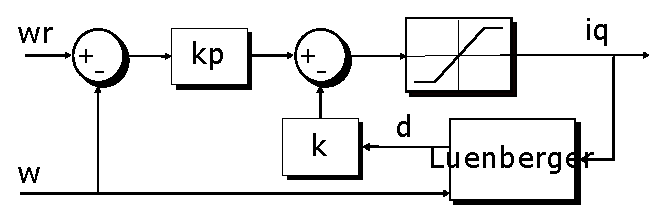
\includegraphics[width=0.485\textwidth]{./figures/speedblock.eps}}\\
\caption{Block diagram of the EXM-CCSMPCC.}
\label{fig:speedblock}
\end{figure}



\subsection{Extended SPMSM Model based Single Step Error Tracking CCS-MPCC}

Let 
\begin{equation}
\label{eq:delta}
\left\{
\begin{align}
\Delta_d={i}_{d}^{*}-{i}_{d} \\
\Delta_q={i}_{q}^{*}-{i}_{q}
\end{align}
\right
\end{equation}



Assume the errors between the given currents and the predicted currents converge exponentially, namely $\Delta_d=e^{-\rho_d t}$, $\Delta_q=e^{-\rho_q t}$. The time derivatives of $\Delta_d$ and $\Delta_q$ can be derived as
\begin{equation}
\label{eq:ddeltadt}
\left\{
\begin{align}
\dot{\Delta}_d &= -\rho_d {\Delta}_d \\
\dot{\Delta}_q &= -\rho_q {\Delta}_q
\end{align}
\right
\end{equation}

Let $\eta_{d}=(1 - T_c \rho_d)$ and $\eta_{q}=(1 - T_c \rho_q)$, and (\ref{eq:ddeltadt}) can be discretized as 
\begin{equation}
\label{eq:ddeltadt_descrite}
\left\{
\begin{align}
\Delta_d(t+1) &= \eta_{d} {\Delta}_d(t) \\
\Delta_q(t+1) &= \eta_{q} {\Delta}_q(t)
\end{align}
\right
\end{equation}
Where $0<\eta_{d}<1$, $0<\eta_{q}<1$.\par
 Therefore, the cost index of the SSET-CCSMPCC is designed as

\begin{equation}
\label{eq:onesteperrorcost}
\begin{align}
J_\Delta(t)&=\lambda_{d0}(\Delta_d(t) \eta_{d}-\Delta_d(t+1))^2\\
		&+\lambda_{q0}(\Delta_q(t) \eta_{q}-\Delta_q(t+1))^2
\end{align}
\end{equation}

If the cost function $J_\Delta(t)$ in (\ref{eq:onesteperrorcost}) is minimized, (\ref{eq:ddeltadt}) is approximately satisfied. Thus the ${\Delta}_d$ and ${\Delta}_q$ converge exponentially.\par

According to (\ref{eq:delta}), it obtains
\begin{equation}
\label{eq:deltadiscretized}
\left\{
\begin{align}
\Delta_d(t)&={i}_{d}^{*}(t)-{i}_{d}(t) \\
\Delta_q(t)&={i}_{q}^{*}(t)-{i}_{q}(t)\\
\Delta_d(t+1)&={i}_{d}^{*}(t+1)-{i}_{d}(t+1) \\
\Delta_q(t+1)&={i}_{q}^{*}(t+1)-{i}_{q}(t+1)
\end{align}
\right
\end{equation}
Substituting (\ref{eq:d_extended_de}) and (\ref{eq:deltadiscretized}) into (\ref{eq:onesteperrorcost}), and sloving $\frac{\partial{J_\Delta(t)}}{\partial{u_{d}^*}(t)}=0$, $\frac{\partial{J_\Delta(t)}}{\partial{u_{q}^*}(t)}=0$, it obtains

\begin{equation}
\label{eq:u_dq}
\left\{
\begin{align}
{u_{d}^*}(t)=\frac{L}{T_c}&(i_d^*(t+1)-\eta_{d} i_d^*(t)\\
					-&(1-\eta_{d}) i_d(t))-T_c \hat{n}_d(t))\\
{u_{q}^*}(t)=\frac{L}{T_c}&(i_q^*(t+1)-\eta_{q} i_q^*(t)\\
					-&(1-\eta_{q}) i_q(t))-T_c \hat{n}_q(t))
\end{align}
\right
\end{equation}
Fig. \ref{fig:sset-ccsmpccblock} shows the block diagram of the SSET-CCSMPCC. In the step response test, large $\eta_{d}$, $\eta_{q}$ will eliminate the overshoots of the $i_d$ and $i_q$, but increase the tracking time and the current ripples. To solve the problem, an MSET-CCSMPCC is proposed in the next section.
\begin{figure}[htbp]
\centering
\psfrag{wr}[c][c][1]{$i_{d}^{*}/i_{q}^{*}$}
\psfrag{w}[c][c][1]{$i_{d}/i_{q}$}
\psfrag{kp}[c][c][1]{$L \frac{1}{T_c}$}
\psfrag{k}[c][c][1]{$L$}
\psfrag{d}[c][c][1]{$\hat{n}_d/\hat{n}_q$}
\psfrag{Luenberger}[c][c][0.8]{$\rm FTSMDO$}
\psfrag{Observer}[c][c][1]{$$}
\psfrag{iq}[l][l][1]{$u_{d}^{*}/u_{q}^{*}$}
\psfrag{y}[c][c][1]{$\eta_{d}/\eta_{q}$}
\psfrag{1-y}[c][c][1]{$1-\eta_{d}/\eta_{q}$}
\psfrag{z-}[c][c][1]{$z^{-1}$}
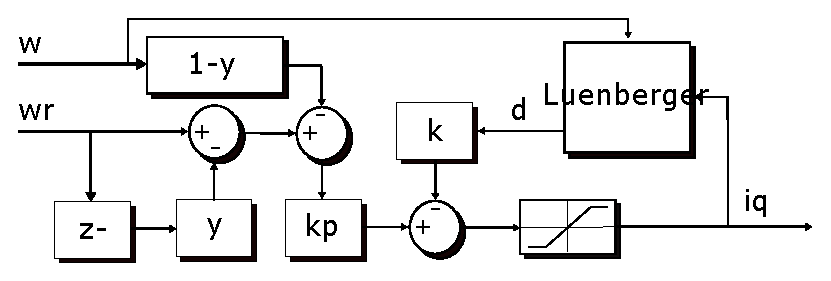
\includegraphics[width=0.485\textwidth]{./figures/SSET-CCSMPCC.eps}}\\
\caption{Block diagram of the SSET-CCSMPCC.}
\label{fig:sset-ccsmpccblock}
\end{figure}


\subsection{Extended SPMSM Model based Multi-step Error Tracking CCS-MPCC}
According to (\ref{eq:ddeltadt_descrite}), it derives

\begin{equation}
\label{eq:mul_ddeltadt_descrite}
\left\{
\begin{align}
\Delta_d(t+1) &= \eta_{d}^{j+1} {\Delta}_d(t-j) \\
\Delta_q(t+1) &= \eta_{q}^{j+1} {\Delta}_q(t-j)
\end{align}
\right
\end{equation}
The cost index of the MSET-CCSMPCC can be constructed as follows.
\begin{equation}
\label{eq:errorcost}
\begin{align}
J_M_\Delta(t)=&\sum\limits_{j=0}^{m-1}\lambda_{dj}(\Delta_d(t-j) \eta_{d}^{j+1}-\Delta_d(t+1))^2\\
		&+\sum\limits_{j=0}^{m-1}\lambda_{qj}(\Delta_q(t-j) \eta_{q}^{j+1}-\Delta_q(t+1))^2
\end{align}
\end{equation}
Where $\Delta_d(t-j)={i}_{d}^{*}(t-j)-{i}_{d}(t-j)$, $\Delta_q(t-j)={i}_{q}^{*}(t-j)-{i}_{q}(t-j)$, and $\Delta_d(t+1)$, $\Delta_q(t+1)$ can be derived by combining (\ref{eq:d_extended_de}) and (\ref{eq:deltadiscretized}). Assuming that each sub-item has the same weight, $\lambda_{dj}$ and $\lambda_{qj}$ can be chosen as 1. By solving $\frac{\partial{J_M_\Delta(t)}}{\partial{u_{d}^*}(t)}=0$ and $\frac{\partial{J_M_\Delta(t)}}{\partial{u_{q}^*}(t)}=0$, the cost index $J_M_\Delta(t)$ in (\ref{eq:errorcost}) is minimized, and the appropriate voltage variables $u_{d}^*(t)$ and $u_{q}^*(t)$ can be calculated as

\begin{equation}
\label{eq:u_dq}
\left\{
\begin{align}
{u_{d}^*}(t)&=\frac{L}{m T_c}(m i_d^*(t+1)-\sum\limits_{j=0}^{m-1}\eta_{d}^{j+1}i_d^*(t-j)\\
					-&(m i_d(t)-\sum\limits_{j=0}^{m-1}\eta_{d}^{j+1}i_d(t-j))-m T_c \hat{n}_d(t))\\
{u_{q}^*}(t)&=\frac{L}{m T_c}(m i_q^*(t+1)-\sum\limits_{j=0}^{m-1}\eta_{q}^{j+1}i_q^*(t-j)\\
					-&(m i_q(t)-\sum\limits_{j=0}^{m-1}\eta_{q}^{j+1}i_q(t-j))-m T_c \hat{n}_q(t))
\end{align}
\right
\end{equation}
In Fig. \ref{fig:mset-ccsmpccblock}, the block diagram of the MSET-CCSMPCC is depicted.
\iffalse
$ \; Analysis \; of \; the \; step \; performance$: 
The (\ref{eq:u_dq}) can be written as
\begin{equation}
\label{eq:u_dq_errpred}
\left\{
\begin{align}
{u_{d}^*}(t)&=\frac{L}{m T_c}((m-\sum\limits_{j=0}^{m-1}\eta_{d}^{j+1})(i_d^*(t+1)-i_d(t))\\
						+&\sum\limits_{j=0}^{m-1}\eta_{d}^{j+1}(i_d^*(t+1)-i_d^*(t-j))\\
						+&\sum\limits_{j=1}^{m-1}\eta_{d}^{j+1}(i_d(t-j)-i_d(t)))-L\hat{n}_d(t)\\
\iffalse
{u_{q}^*}(t)&=\frac{L}{m T_c}((m-\sum\limits_{j=0}^{m-1}\eta_{q}^{j+1})(i_q^*(t+1)-i_q(t))\\
						+&\sum\limits_{j=0}^{m-1}\eta_{q}^{j+1}(i_q^*(t+1)-i_q^*(t-j))\\
						+&\sum\limits_{j=1}^{m-1}\eta_{q}^{j+1}(i_q(t-j)-i_q(t)))-L\hat{n}_q(t)
\fi
\end{align}
\right
\end{equation}


At the beginning of the step test, $\sum\limits_{j=0}^{m-1}\eta_{d}^{j+1}(i_d^*(t+1)-i_d^*(t-j))-\sum\limits_{j=0}^{m-1}\eta_{d}^{j+1}(i_d^*(t+1)-i_d(t-j))=0$, so (\ref{eq:u_dq_errpred}) is equal to (\ref{eq:improved_ccsmpc}), which is the fastest. When the time is more than $m$ periods, $\sum\limits_{j=0}^{m-1}\eta_{d}^{j+1}(i_d^*(t+1)-i_d^*(t-j))=0$, and the gain of the error is reduced by $\sum\limits_{j=0}^{m-1}\eta_{d}^{j+1}$, and the output of $u_d^*$ is even reduced by the  $i_d(t-j)-i_d(t)$ item. From $0$ to $m$ periods, the gain of the error is reduced slowly.




\fi

\begin{figure}[htbp]
\def\size{0.5}
\centering
\psfrag{wr}[r][r][\size]{$i_{d}^{*}/i_{q}^{*}$}
\psfrag{w}[c][c][\size]{$i_{d}/i_{q}$}
\psfrag{kp}[c][c][\size]{$L \frac{1}{T_c}$}
\psfrag{k}[c][c][\size]{$L$}
\psfrag{d}[c][c][\size]{$\hat{n}_d/\hat{n}_q$}
\psfrag{Luenberger}[c][c][\size]{$\rm FTSMDO$}
\psfrag{Observer}[c][c][\size]{$$}
\psfrag{iq}[l][l][\size]{$u_{d}^{*}/u_{q}^{*}$}
\psfrag{y}[c][c][\size]{$\eta_{d}/\eta_{q}$}
\psfrag{m-y}[c][c][\size]{$m-\eta_{d}/\eta_{q}$}
\psfrag{m}[c][c][\size]{$m$}
\psfrag{y2}[c][c][\size]{$\eta_{d}^{2}/\eta_{q}^{2}$}
\psfrag{yj+1}[c][c][\size]{$\eta_{d}^{j+1}/\eta_{q}^{j+1}$}
\psfrag{ym}[c][c][\size]{$\eta_{d}^{m}/\eta_{q}^{m}$}
\psfrag{yj}[c][c][\size]{$\eta_{d}^{j}/\eta_{q}^{j}$}
\psfrag{z1}[c][c][\size]{$z^{-1}$}
\psfrag{zj}[c][c][\size]{$z^{-j}$}
\psfrag{zm}[c][c][\size]{$z^{-m}$}
\psfrag{zm-1}[c][c][\size]{$z^{-(m-1)}$}


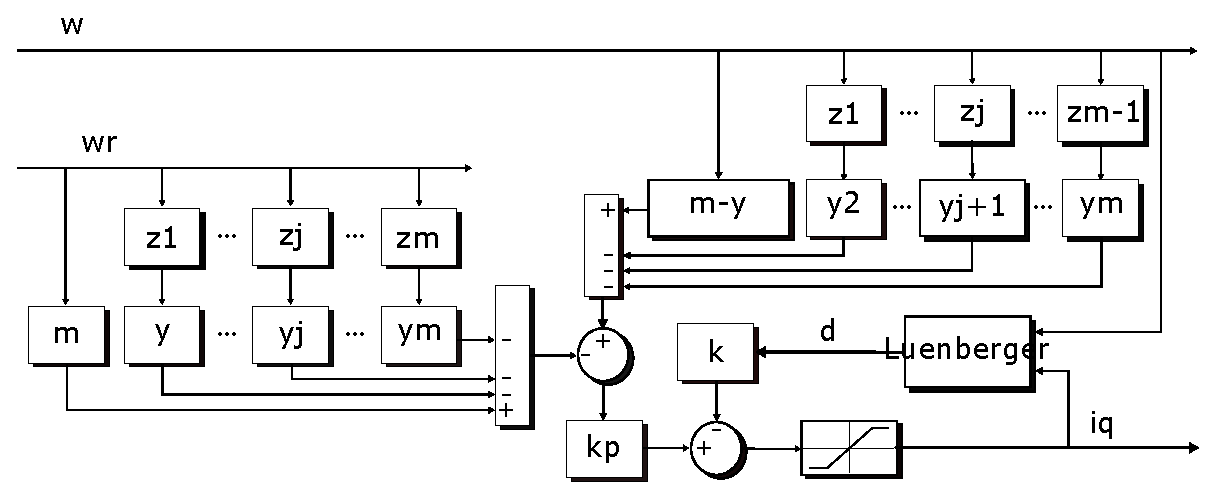
\includegraphics[width=0.485\textwidth]{./figures/MSET-CCSMPCC.eps}}\\
\caption{Block diagram of the MSET-CCSMPCC.}
\label{fig:mset-ccsmpccblock}
\end{figure}


\begin{figure}[htbp]
\def\size{0.7}
\def\sizetwo{0.5}
\centering
\psfrag{Router}[c][c][\size]{$\rm Load \; Inverter$}
\psfrag{PC}[c][c][\size]{$\rm P C$}
\psfrag{JTAG}[c][c][\size]{$\rm S h a f t$}
\psfrag{CPU0}[c][c][\size]{$\rm C  P  U  0$}
\psfrag{L}[c][c][\sizetwo]{$\rm (Embedded \; Linux)$}
\psfrag{CPU1}[c][c][\size]{$\rm C P  U  1$}
\psfrag{R}[c][c][\sizetwo]{$\rm (Motor \; Control)$}
\psfrag{Z}[c][c][\size]{$\rm X  C7Z020  \!  -  \! C  L  G484  \!  -  \!  1$}
%\psfrag{B}[c][c][\size]{$(L \! D \! O \! B \! - \! S \! P \! D \! C)$}
\psfrag{AXI}[c][c][\size]{$\rm A  X  I$}
\psfrag{PWM}[c][c][\size]{$\rm P  W  M$}
\psfrag{G}[c][c][\size]{$\rm Generator$}
\psfrag{S}[c][c][\size]{$\rm OCM \; (Circular \; Queues)$}
\psfrag{D1}[c][c][\size]{$\rm Current  \; Loop$}
\psfrag{D2}[c][c][\sizetwo]{$\rm (L  D  O  B  \!  -  \!  D  P  C  C/D  P  C  C)$}
\psfrag{PWM}[c][c][\size]{$\rm P  W  M$}
\psfrag{ADC}[c][c][\size]{$\rm A  D  C$}
\psfrag{I}[c][c][\size]{$\rm Interface$}
\psfrag{Encoder}[c][c][\size]{$\rm Encoder$}
\psfrag{D}[c][c][\size]{$\rm Decoding$}
\psfrag{A,B}[c][c][\size]{$\rm A,B$}
\psfrag{PMSM}[c][c][\size]{$\rm \bf{P  M  S  M}$}
\psfrag{A/D}[c][c][\size]{$\rm A/D$}
\psfrag{Sa,Sb,Sc}[c][c][\size]{$\rm S_a,S_b,S_c$}
\psfrag{V}[c][c][\size]{$\rm 300V$}
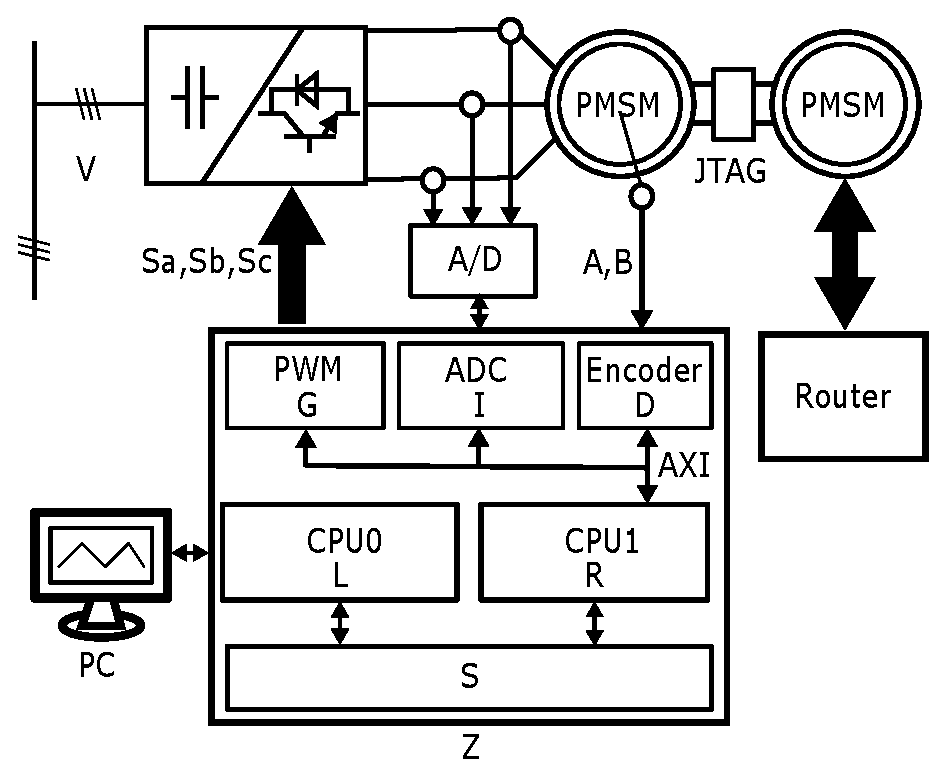
\includegraphics[width=0.49\textwidth]{./figures/blockdiagram.eps}}\\
\caption{Block diagram of the designed FPGA-based hardware system.}
\label{fig:blockdiagram}
\end{figure}


\begin{figure}[htbp]
\def\size{0.9}
\centering
\psfrag{I}[c][c][\size]{$\rm Load  \; Inverter$}
\psfrag{Zynq}[c][c][\size]{$\rm Zynq  \; Inverter$}
\psfrag{L}[c][c][\size]{$\rm Load  \; Motor$}
\psfrag{D}[c][c][\size]{$\rm Drive  \; Motor$}
\psfrag{pc}[c][c][\size]{$\rm PC  \; with \; Monitor$}
\psfrag{m}[c][c][\size]{$\rm Monitor$}
\psfrag{R}[c][c][\size]{$\rm Router$}
\includegraphics[width=0.485\textwidth]{./figures/testbench.eps}}\\
\caption{Experimental setup description.}
\label{fig:experiment}
\end{figure}

\section{Experimental Results}
An FPGA-based hardware system has been designed as shown in Fig. \ref{fig:blockdiagram}. The XC7Z020-CLG484-1, which incorporates dual-core Cortex-A9 processors and an FPGA core, was utilized as the control unit. A pulse-width modulation (PWM) Generator, an analog-to-digital converter (ADC) interface, an Encoder Decoding are implemented on the FPGA core by employing verilog language. By properly designing the PWM Generator module clock, a desired resolution is achieved. A parallel interface is designed to interface to a 16-bit, simultaneous sampling ADC AD7606. The Encoder Decoding is designed to interface to an incremental encoder, which provides information on the sensor's current position and the period between two encoder events. 
\iffalse
FPGA implemented hardware system has several advantages, including:

			\begin{itemize}
			\item Flexible input and output (IO) layout facilitates schematic design and printed circuit board (PCB) design.
			\item The software can be designed more efficiently for a dedicated FPGA-based hardware. The universal micro-controller units (MCUs) and digital signal processors (DSPs) usually have unused and required functions incorporated in one module, which increases the software complexity.
			\item Many advanced applications can be incorporated into the dedicated FPGA-based hardware as well, such as digital filter, digital noise reduction, which improve the system performances. 
			\end{itemize}
\fi
CPU0 (CPU: central processing unit), which runs an embeded linux, communicates with a control and monitoring software installed on the computer via Ethernet. The motor control algorithms are implemented on the CPU1, which communicates with the CPU0 via the on chip memory (OCM).\par
To verify the proposed algorithms, an SPMSM test bench has been established as shown in Fig. \ref{fig:experiment}. Two SPMSMs made by Wenling Yuhai Electromechanical Corporation with the parameters specified in Table \ref{parameters} are coupled via a flexible coupling. The drive motor which is driven by an FPGA-based hardware system, is used to test the algorithms. And the load motor which is driven by a $\rm 3.0 \; kW$ commercial inverter made by Micno Corporation, is applied to provide the speed. An incremental encoder with a resolution of 2500 pulses per revolution (P/R) is utilized for measuring the SPMSM speed. Three high precision sampling resistors are used to measure the stator currents.\par
In the following sections, experimental results are presented and analyzed. In the section A, the proposed methods are tested to verify the effectiveness. In the section B, the performances of the designed FTSMDO are verified. In the section C and D, the proposed methods are explicitly compared with the existed conventional CCS-MPCC for sharing the advantages and drawbacks.
% , and the speed loop operates at $\rm 1.25 \; kHz$

\begin{table}[!t]
	\renewcommand{\arraystretch}{1.3}
	\caption{PARAMETERS OF SPMSM}  %表格的名字
	\centering
	\label{parameters}
	%\centering
	\resizebox{\columnwidth}{!}{
	\begin{tabular}{{l  l  l}}  % 表格开始,两个C表示分为两列
			\hline\hline \\[-3mm]
Descriptions & Parameters & Nominal Values\\    %表头
\hline     %一道分隔线
Stator resistance & $R$                     & 1.7912 $\Omega$ \\   %数据
Stator inductance &  $L$                     & 3.5 $mH$ \\        %单元分割
Pole pairs &  $p$                      & 4  \\
PM flux &  $\lambda$          & 0.0799 $Vs$ \\
Rated power &  $P_N$               & 0.75 $kW$\\
Rotor inertia &  $J_n$                      & 0.00024 $Kg \cdot m^2$\\
Rated current & $I_N$ (eff.)       & 3.5 $A$\\
Rated speed &  $\omega_{M \! N}$			& 3000 $rpm$\\
Rated voltage &  $U_N$ (eff.)   & 220 $V$\\
Rated torque &  $T_{M \! N}$  & 2.4 $Nm$\\
DC link voltage &  $V_{dc}$ & 300 $V$\\
		[1.4ex] \hline\hline
		\end{tabular}
	}
\end{table}



\subsection{Speed Reversal Performance}
Experiments to validate the performances of the EXM-CCSMPC and MSET-CCSMPCC during the rated full-speed range are carried out respectively in Figs. \ref{et_reverse} and \ref{edb_reverse}, where the load motor is out of service and the $\omega_m^*$ is directly changed in the program. In both experiments, the PI control with the same parameters is applied to the outer speed loop, and the given speed $\omega_m^*$ is changed from $\rm 3000   \; rpm$ to $\rm -3000   \; rpm$ at 0.16s. The q-axis currents of both methods jump to their upper bounds within $\rm 3 \; ms$, but the $i_q$ overshoot of MSET-CCSMPCC (almost no overshoot) is much smaller than that of EXM-CCSMPC (0.8A overshoot). As $i_q$ is proportional to the electromagnetic torque, the drive SPMSM reverses from $\rm 3000   \; rpm$ to $\rm -3000   \; rpm$ fast in both experiments (within $\rm 0.09 s$). The experimental results indicate the proposed EXM-CCSMPCC and MSET-CCSMPCC have fast dynamic response in the full-speed range. However, the MSET-CCSMPCC has better performance considering the overshoot suppression.


\begin{figure}[htbp]
\def\size{0.6}
\def\sizetwo{0.45}
\centering
\psfrag{0}[tc][tc][\size]{$\bm{0}$}
\psfrag{0.05}[tc][tc][\size]{$\bm{0.05}$}
\psfrag{0.15}[tc][tc][\size]{$\bm{0.15}$}
\psfrag{0.25}[tc][tc][\size]{$\bm{0.25}$}
\psfrag{0.35}[tc][tc][\size]{$\bm{0.35}$}

\psfrag{0.1}[tc][tc][\size]{$\bm{0.1}$}
\psfrag{0.2}[tc][tc][\size]{$\bm{0.2}$}
\psfrag{0.3}[tc][tc][\size]{$\bm{0.3}$}
\psfrag{0.4}[tc][tc][\size]{$\bm{0.4}$}
\psfrag{0.5}[tc][tc][\size]{$\bm{0.5}$}
\psfrag{0.6}[tc][tc][\size]{$\bm{0.6}$}
\psfrag{0.7}[tc][tc][\size]{$\bm{0.7}$}
\psfrag{0.8}[tc][tc][\size]{$\bm{0.8}$}
\psfrag{0.9}[tc][tc][\size]{$\bm{0.9}$}
\psfrag{1}[tc][tc][\size]{$\bm{1}$}
\psfrag{-7.0}[r][r][\size]{$\bm{-7}$}
\psfrag{7.0}[r][r][\size]{$\bm{7}$}
\psfrag{-7}[r][r][\size]{$\bm{-7}$}
\psfrag{7}[r][r][\size]{$\bm{7}$}
\psfrag{0.0}[r][r][\size]{$\bm{0}$}
\psfrag{2.0}[r][r][\size]{$\bm{2}$}
\psfrag{2}[r][r][\size]{$\bm{2}$}
\psfrag{-4000}[r][r][\size]{$\bm{-4000}$}
\psfrag{4000}[r][r][\size]{$\bm{4000}$}

\psfrag{-4000.0}[r][r][\size]{$\bm{-4000}$}
\psfrag{4000.0}[r][r][\size]{$\bm{4000}$}
\psfrag{t}[tc][tc][\size]{$\rm \textbf{Time  \; [s]}$}
\psfrag{d}[bc][bc][\size]{$\bm{\omega_m}  \; \rm \textbf{[rpm]}$}
\psfrag{b}[bc][bc][\size]{$\bm{i_q}  \; \rm \textbf {[A]}$}
\psfrag{a}[bc][bc][\size]{$\bm{i_a}  \; \rm \textbf {[A]}$}
\psfrag{c}[bc][bc][\size]{$\bm{i_d}  \; \rm \textbf {[A]}$}

\psfrag{0.00}[c][c][\sizetwo]{$\bm{0}$}
\psfrag{-5.00}[c][c][\sizetwo]{$\bm{-5}$}
\psfrag{0.495}[c][c][\sizetwo]{$\bm{0.495}$}
\psfrag{0.502}[l][l][\sizetwo]{$\bm{0.502}$}
\psfrag{0.547}[c][c][\sizetwo]{$\bm{0.547}$}
\psfrag{0.554}[l][l][\sizetwo]{$\bm{0.554}$}

\psfrag{0.158}[c][c][\sizetwo]{$\bm{0.158}$}
\psfrag{0.165}[l][l][\sizetwo]{$\bm{0.165}$}
\psfrag{0.249}[c][c][\sizetwo]{$\bm{0.249}$}
\psfrag{0.255}[l][l][\sizetwo]{$\bm{0.255}$}

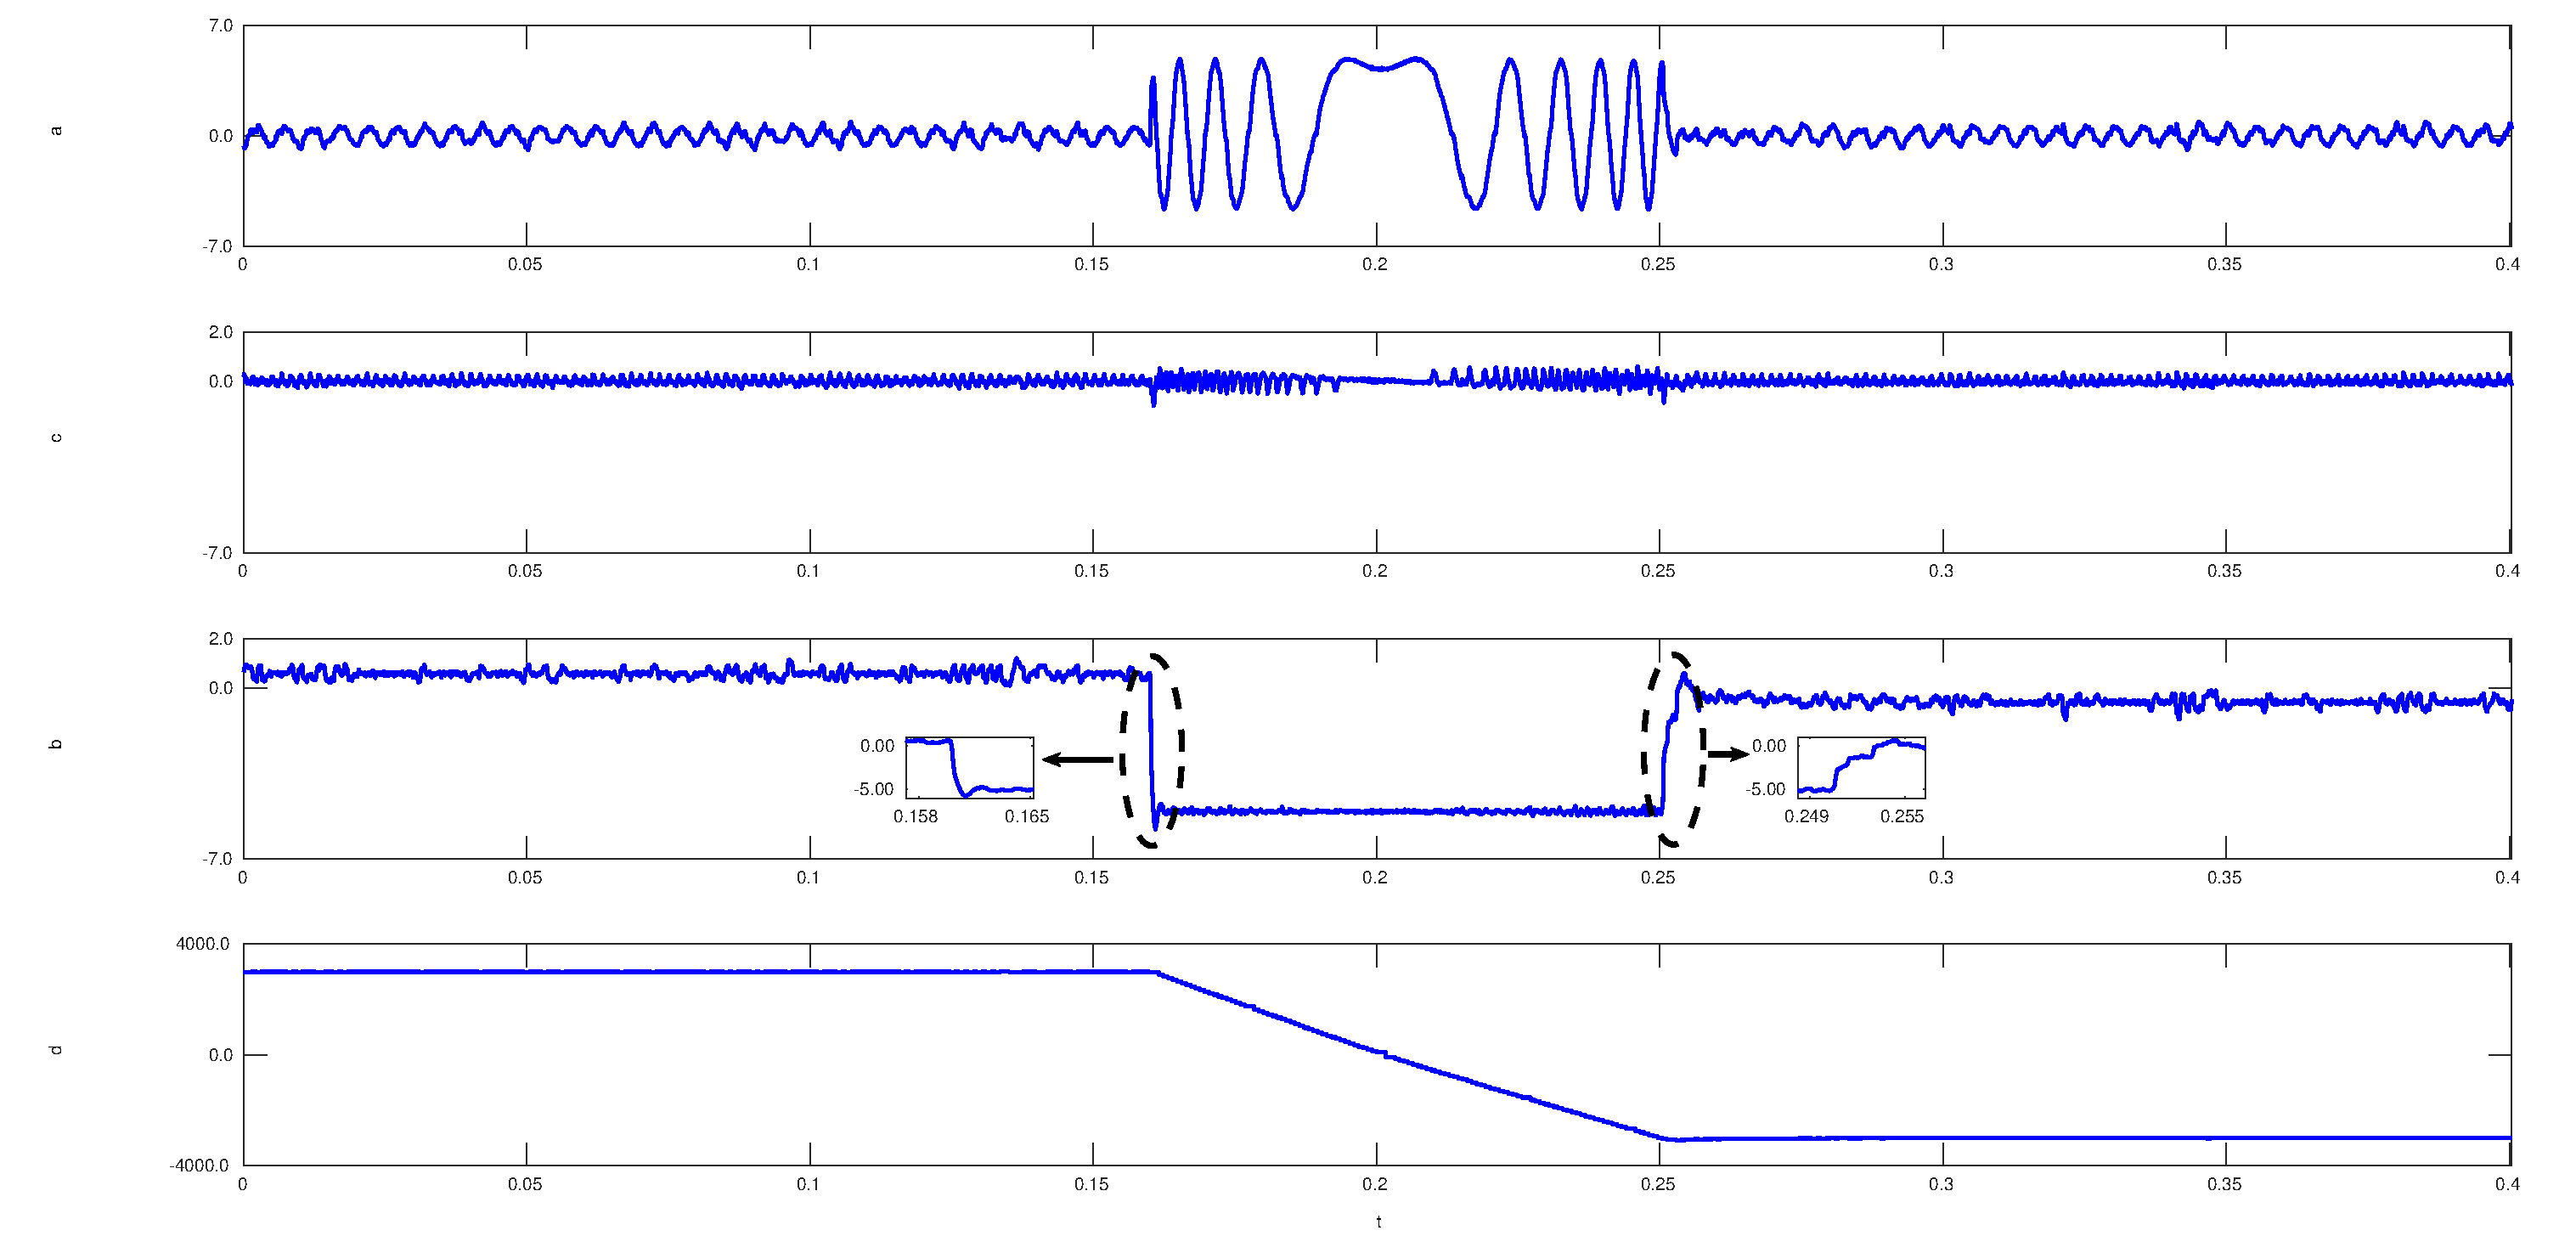
\includegraphics[width=0.49\textwidth]{./figures/edb_reverse.eps}\\
\caption{Experimental results during the rated full-speed reversal process. (PI cascade with EXM-CCSMPC, from $\rm 3000 \; rpm$ to $\rm -3000 \; rpm$).}
\label{edb_reverse}
\end{figure}

\begin{figure}[htbp]
\def\size{0.6}
\def\sizetwo{0.45}
\centering
\psfrag{0}[tc][tc][\size]{$\bm{0}$}
\psfrag{0.05}[tc][tc][\size]{$\bm{0.05}$}
\psfrag{0.15}[tc][tc][\size]{$\bm{0.15}$}
\psfrag{0.25}[tc][tc][\size]{$\bm{0.25}$}
\psfrag{0.35}[tc][tc][\size]{$\bm{0.35}$}

\psfrag{0.1}[tc][tc][\size]{$\bm{0.1}$}
\psfrag{0.2}[tc][tc][\size]{$\bm{0.2}$}
\psfrag{0.3}[tc][tc][\size]{$\bm{0.3}$}
\psfrag{0.4}[tc][tc][\size]{$\bm{0.4}$}
\psfrag{0.5}[tc][tc][\size]{$\bm{0.5}$}
\psfrag{0.6}[tc][tc][\size]{$\bm{0.6}$}
\psfrag{0.7}[tc][tc][\size]{$\bm{0.7}$}
\psfrag{0.8}[tc][tc][\size]{$\bm{0.8}$}
\psfrag{0.9}[tc][tc][\size]{$\bm{0.9}$}
\psfrag{1}[tc][tc][\size]{$\bm{1}$}
\psfrag{-7.0}[r][r][\size]{$\bm{-7}$}
\psfrag{7.0}[r][r][\size]{$\bm{7}$}
\psfrag{-7}[r][r][\size]{$\bm{-7}$}
\psfrag{7}[r][r][\size]{$\bm{7}$}
\psfrag{0.0}[r][r][\size]{$\bm{0}$}
\psfrag{2.0}[r][r][\size]{$\bm{2}$}
\psfrag{2}[r][r][\size]{$\bm{2}$}
\psfrag{-4000}[r][r][\size]{$\bm{-4000}$}
\psfrag{4000}[r][r][\size]{$\bm{4000}$}

\psfrag{-4000.0}[r][r][\size]{$\bm{-4000}$}
\psfrag{4000.0}[r][r][\size]{$\bm{4000}$}
\psfrag{t}[tc][tc][\size]{$\rm \textbf{Time  \; [s]}$}
\psfrag{d}[bc][bc][\size]{$\bm{\omega_m}  \; \rm \textbf{[rpm]}$}
\psfrag{b}[bc][bc][\size]{$\bm{i_q}  \; \rm \textbf {[A]}$}
\psfrag{a}[bc][bc][\size]{$\bm{i_a}  \; \rm \textbf {[A]}$}
\psfrag{c}[bc][bc][\size]{$\bm{i_d}  \; \rm \textbf {[A]}$}

\psfrag{0.00}[c][c][\sizetwo]{$\bm{0}$}
\psfrag{-5.00}[c][c][\sizetwo]{$\bm{-5}$}
\psfrag{0.495}[c][c][\sizetwo]{$\bm{0.495}$}
\psfrag{0.502}[l][l][\sizetwo]{$\bm{0.502}$}
\psfrag{0.547}[c][c][\sizetwo]{$\bm{0.547}$}
\psfrag{0.554}[l][l][\sizetwo]{$\bm{0.554}$}

\psfrag{0.155}[c][c][\sizetwo]{$\bm{0.155}$}
\psfrag{0.161}[l][l][\sizetwo]{$\bm{0.161}$}
\psfrag{0.251}[c][c][\sizetwo]{$\bm{0.251}$}
\psfrag{0.257}[l][l][\sizetwo]{$\bm{0.257}$}

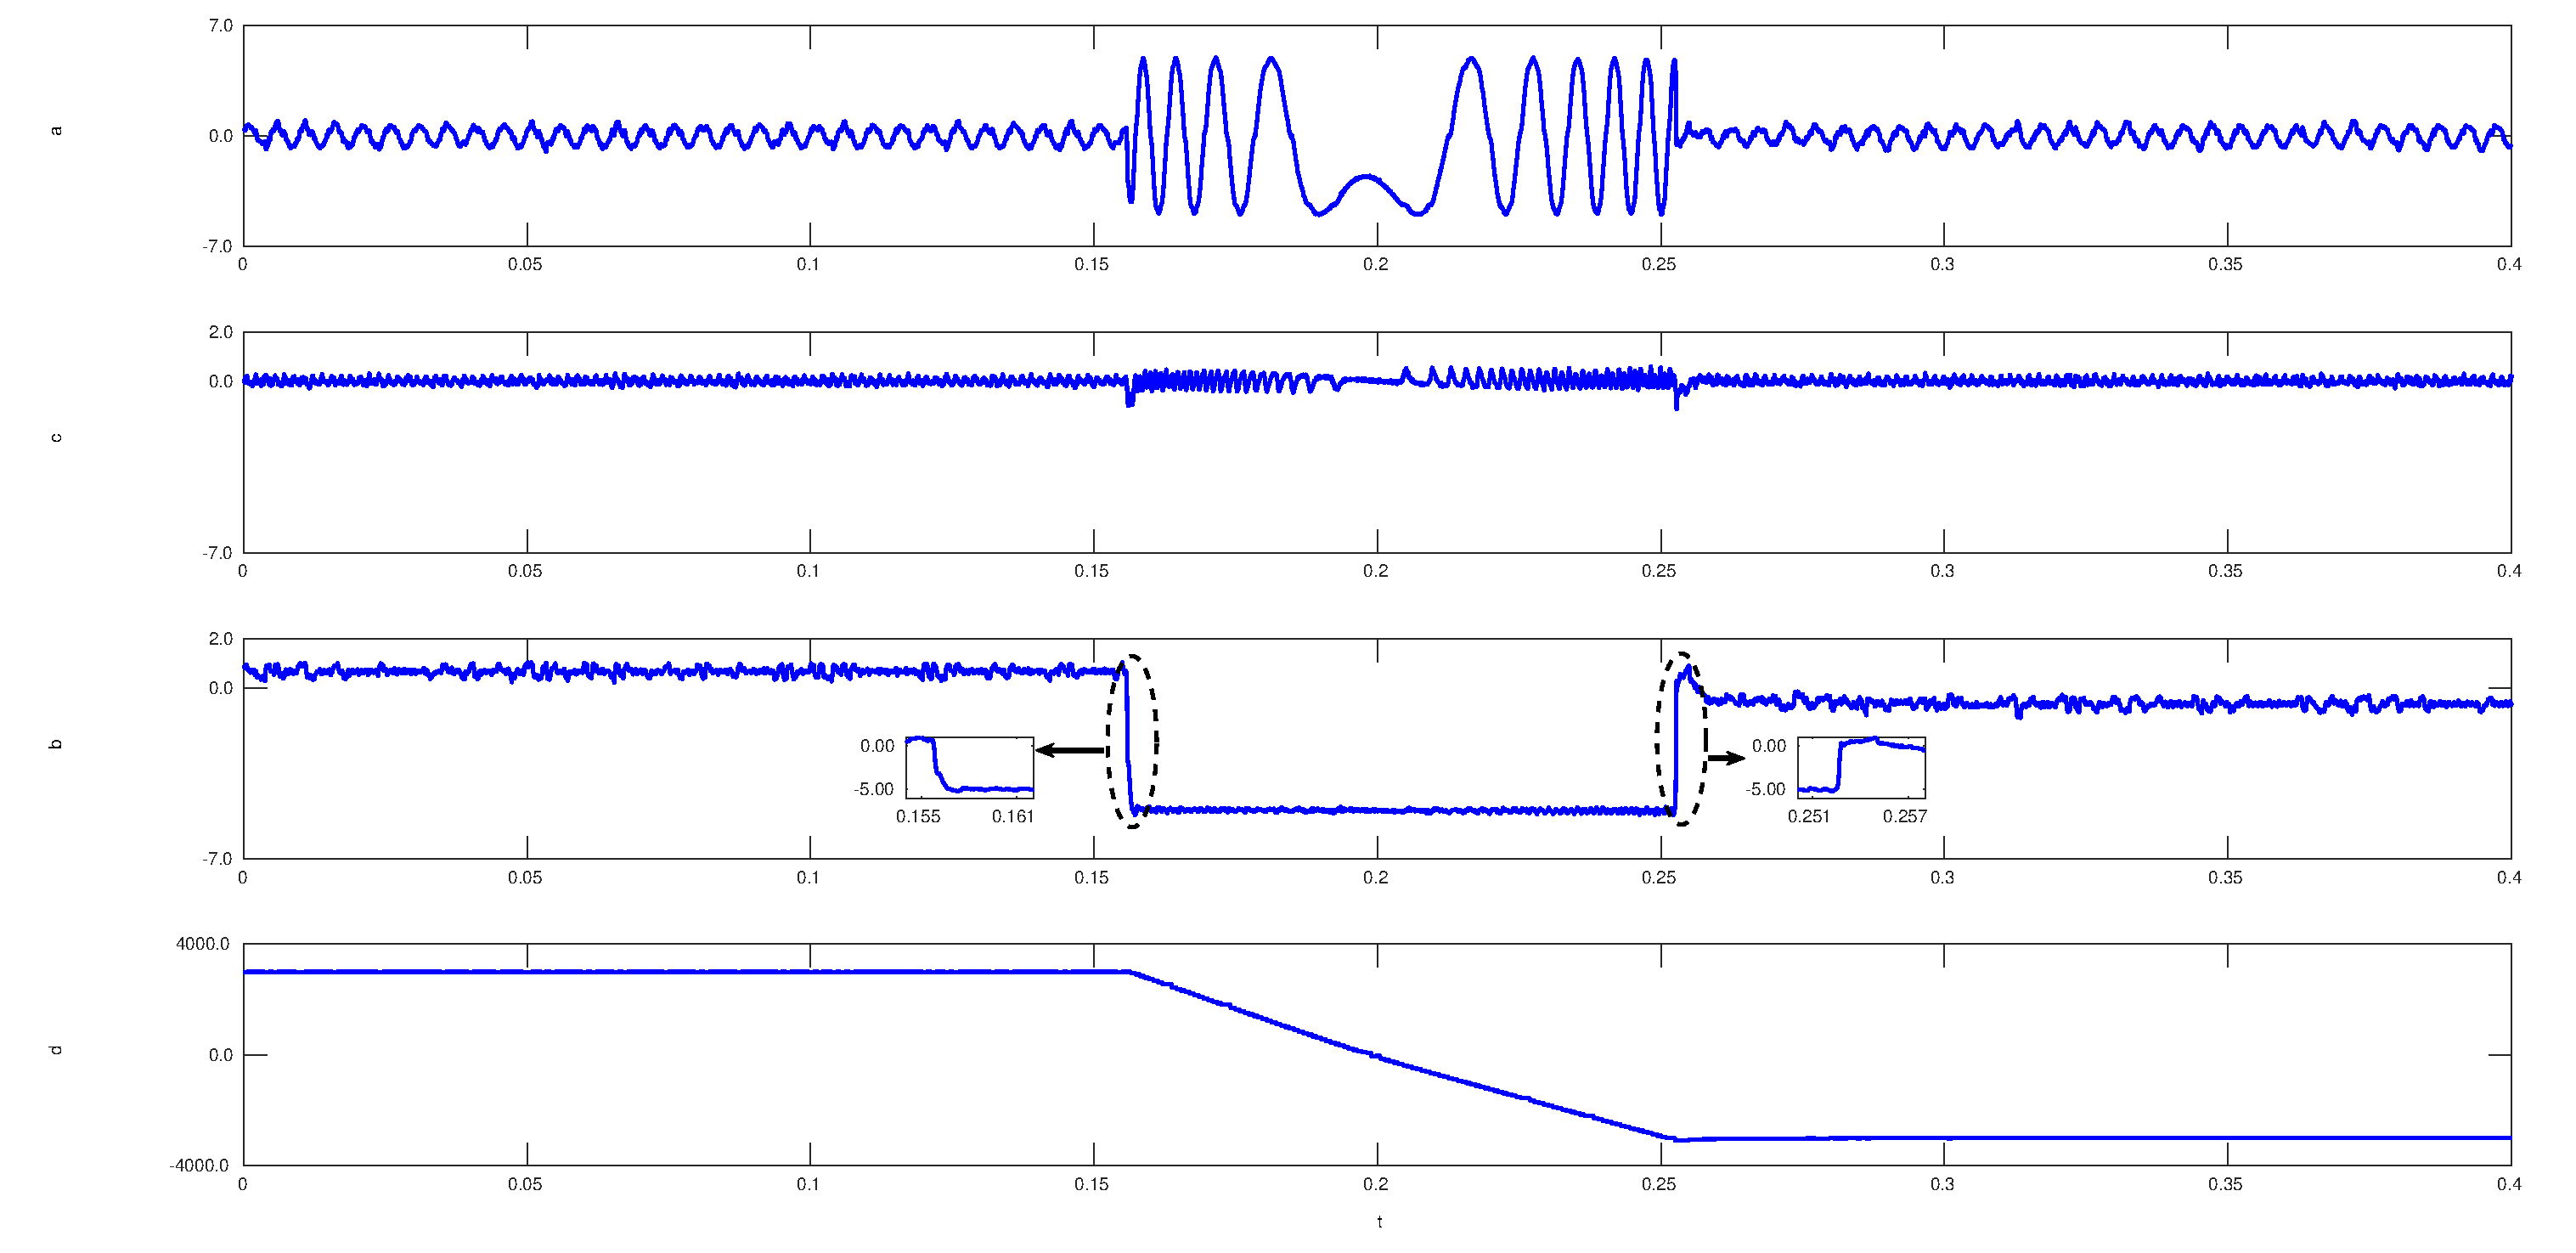
\includegraphics[width=0.49\textwidth]{./figures/et_reverse.eps}\\
\caption{Experimental results during the rated full-speed reversal process. (PI cascade with MSET-CCSMPCC, from $\rm 3000 \; rpm$ to $\rm -3000 \; rpm$).}
\label{et_reverse}
\end{figure}

\subsection{Performance of FTSMDO}
To verify the excellent performances of the designed FTSMDO, an exponential reaching law based SMDO is given below as a comparison method.

\begin{equation}
\label{eq:exp_smdo}
\left\{
\begin{align}
\dot{\hat{i}}_q &= \frac{{u}_{q}^*}{L}+\hat{n}_q+\alpha_q e_q + \beta_q {\rm sign}(e_q)\\
\dot{\hat{n}}_q &= \alpha_{nq} (\alpha_q e_q + \beta_q {\rm sign}(e_q))
\end{align}
\right
\end{equation}


Experiments to validate the performances of the SMDO and FTSMDO during the $i_q$ step response test are carried out in Figs. \ref{current_estimate} and \ref{disturbance_estimate}, where the $i_q^*$ is directly changed in the program and the motor speed is provided by the Micno commercial inverter. The conventional CCS-MPCC is applied to the current loop of the FPGA-based hardware system, and the $i_q$ and $u_q^*$ are fed back to the SMDO and FTSMDO respectively. The drive motor runs at $\rm 450 \; rpm$, and the $i_q^*$ is changed from 0A to $\rm 5A$. It can be seen that the FTSMDO tracks slightly faster than the SMDO, and the $\hat{n}_q$ and $\hat{i}_q$ of the SMDO have more serious chatter than that of the FTSMDO (approximately 2 times larger).


\begin{figure}[htbp]
\def\size{0.6}
\def\sizetwo{0.45}
\centering
\psfrag{0}[tc][tc][\size]{$\bm{0}$}
\psfrag{0.05}[tc][tc][\size]{$\bm{0.05}$}
\psfrag{0.15}[tc][tc][\size]{$\bm{0.15}$}
\psfrag{0.25}[tc][tc][\size]{$\bm{0.25}$}
\psfrag{0.35}[tc][tc][\size]{$\bm{0.35}$}

\psfrag{0.1}[tc][tc][\size]{$\bm{0.1}$}
\psfrag{0.2}[tc][tc][\size]{$\bm{0.2}$}
\psfrag{0.3}[tc][tc][\size]{$\bm{0.3}$}
\psfrag{0.4}[tc][tc][\size]{$\bm{0.4}$}
\psfrag{0.5}[tc][tc][\size]{$\bm{0.5}$}
\psfrag{0.6}[tc][tc][\size]{$\bm{0.6}$}
\psfrag{0.7}[tc][tc][\size]{$\bm{0.7}$}
\psfrag{0.8}[tc][tc][\size]{$\bm{0.8}$}
\psfrag{0.9}[tc][tc][\size]{$\bm{0.9}$}
\psfrag{1}[tc][tc][\size]{$\bm{1}$}
\psfrag{-4.00}[r][r][\size]{$\bm{-4}$}
\psfrag{4.00}[r][r][\size]{$\bm{4}$}
\psfrag{-4}[r][r][\size]{$\bm{-4}$}
\psfrag{4.0}[r][r][\size]{$\bm{4}$}
\psfrag{-4.0}[r][r][\size]{$\bm{-4}$}
\psfrag{4}[r][r][\size]{$\bm{4}$}
\psfrag{2.00}[r][r][\sizetwo]{$\bm{2}$}
\psfrag{0.00}[c][c][\sizetwo]{$\bm{0}$}
\psfrag{5.500}[c][c][\sizetwo]{$\bm{5.5}$}
\psfrag{4.500}[c][c][\sizetwo]{$\bm{4.5}$}

\psfrag{0.053}[tc][tc][\sizetwo]{$\bm{0.053}$}
\psfrag{0.057}[tc][tc][\sizetwo]{$\bm{0.057}$}
\psfrag{0.0520}[tc][tc][\sizetwo]{$\bm{0.052}$}
\psfrag{0.0525}[tc][tc][\sizetwo]{$\bm{0.0525}$}
\psfrag{7.500}[tc][tc][\sizetwo]{$\bm{7.5}$}

\psfrag{800}[r][r][\size]{$\bm{800}$}
\psfrag{400}[r][r][\size]{$\bm{400}$}
\psfrag{600}[r][r][\size]{$\bm{600}$}
\psfrag{800.0}[r][r][\size]{$\bm{800}$}
\psfrag{400.0}[r][r][\size]{$\bm{400}$}
\psfrag{600.0}[r][r][\size]{$\bm{600}$}


\psfrag{-120.0}[r][r][\size]{$\bm{-120}$}
\psfrag{-70.0}[r][r][\size]{$\bm{-70}$}
\psfrag{-20.0}[r][r][\size]{$\bm{-20}$}
\psfrag{-1.0}[r][r][\size]{$\bm{-1}$}
\psfrag{9.0}[r][r][\size]{$\bm{9}$}
\psfrag{7.5}[r][r][\size]{$\bm{7.5}$}
\psfrag{3.2}[r][r][\size]{$\bm{3.2}$}

\psfrag{0.01}[tc][tc][\size]{$\bm{0.01}$}
\psfrag{0.02}[tc][tc][\size]{$\bm{0.02}$}
\psfrag{0.03}[tc][tc][\size]{$\bm{0.03}$}

\psfrag{0.04}[tc][tc][\size]{$\bm{0.04}$}
\psfrag{0.06}[tc][tc][\size]{$\bm{0.06}$}
\psfrag{0.07}[tc][tc][\size]{$\bm{0.07}$}

\psfrag{0.08}[tc][tc][\size]{$\bm{0.08}$}
\psfrag{0.09}[tc][tc][\size]{$\bm{0.09}$}


\psfrag{-105.00}[r][r][\sizetwo]{$\bm{-105}$}
\psfrag{-111.00}[r][r][\sizetwo]{$\bm{-111}$}
\psfrag{0.058}[c][c][\sizetwo]{$\bm{0.058}$}
\psfrag{0.061}[c][c][\sizetwo]{$\bm{0.061}$}

\psfrag{0.208}[c][c][\sizetwo]{$\bm{0.208}$}
\psfrag{0.212}[c][c][\sizetwo]{$\bm{0.212}$}
\psfrag{4.75}[r][r][\sizetwo]{$\bm{4.75}$}
\psfrag{5.20}[r][r][\sizetwo]{$\bm{5.2}$}

\psfrag{data1}[l][l][\sizetwo]{$\bm{\hat{i}_q} \rm (SMDO)$}
\psfrag{iq(FTSMDO)}[l][l][\sizetwo]{$\bm{\hat{i}_q} \rm (FTSMDO)$}
\psfrag{data3}[l][l][\sizetwo]{$\bm{{i}_q}$}

\psfrag{2.0}[c][c][\sizetwo]{$\bm{2}$}
\psfrag{0.0}[c][c][\size]{$\bm{0}$}
\psfrag{0.612}[c][c][\sizetwo]{$\bm{0.612}$}
\psfrag{0.614}[l][l][\sizetwo]{$\bm{0.614}$}

\psfrag{2.00}[c][c][\sizetwo]{$\bm{2}$}
\psfrag{0.00}[c][c][\sizetwo]{$\bm{0}$}
\psfrag{0.200}[c][c][\sizetwo]{$\bm{0.2}$}
\psfrag{0.202}[l][l][\sizetwo]{$\bm{0.202}$}

\psfrag{0.70}[c][c][\sizetwo]{$\bm{0.7}$}
\psfrag{0.90}[l][l][\sizetwo]{$\bm{0.9}$}
\psfrag{1.7}[r][r][\sizetwo]{$\bm{1.7}$}
\psfrag{2.3}[r][r][\sizetwo]{$\bm{2.3}$}
\psfrag{0.300}[c][c][\sizetwo]{$\bm{0.3}$}
\psfrag{0.38}[l][l][\sizetwo]{$\bm{0.38}$}
\psfrag{0.310}[c][c][\sizetwo]{$\bm{0.31}$}
\psfrag{0.320}[c][c][\sizetwo]{$\bm{0.32}$}
\psfrag{0.39}[l][l][\sizetwo]{$\bm{0.39}$}

\psfrag{1.70}[r][r][\sizetwo]{$\bm{1.7}$}
\psfrag{2.30}[r][r][\sizetwo]{$\bm{2.3}$}


\psfrag{t}[tc][tc][\size]{$\rm \textbf{Time  \; [s]}$}
\psfrag{b}[c][c][\size]{$\bm{\omega_m}  \; \rm \textbf{[rpm]}$}
\psfrag{c}[c][c][\size]{$\bm{i_q/\hat{i}_q}  \; \rm \textbf {[A]}$}
\psfrag{a}[c][c][\size]{$\bm{\hat{n}_q}  \; \rm \textbf {[V]}$}
%\psfrag{b}[c][c][\size]{$\bm{i_q}  \; \rm \textbf {[A]}$}
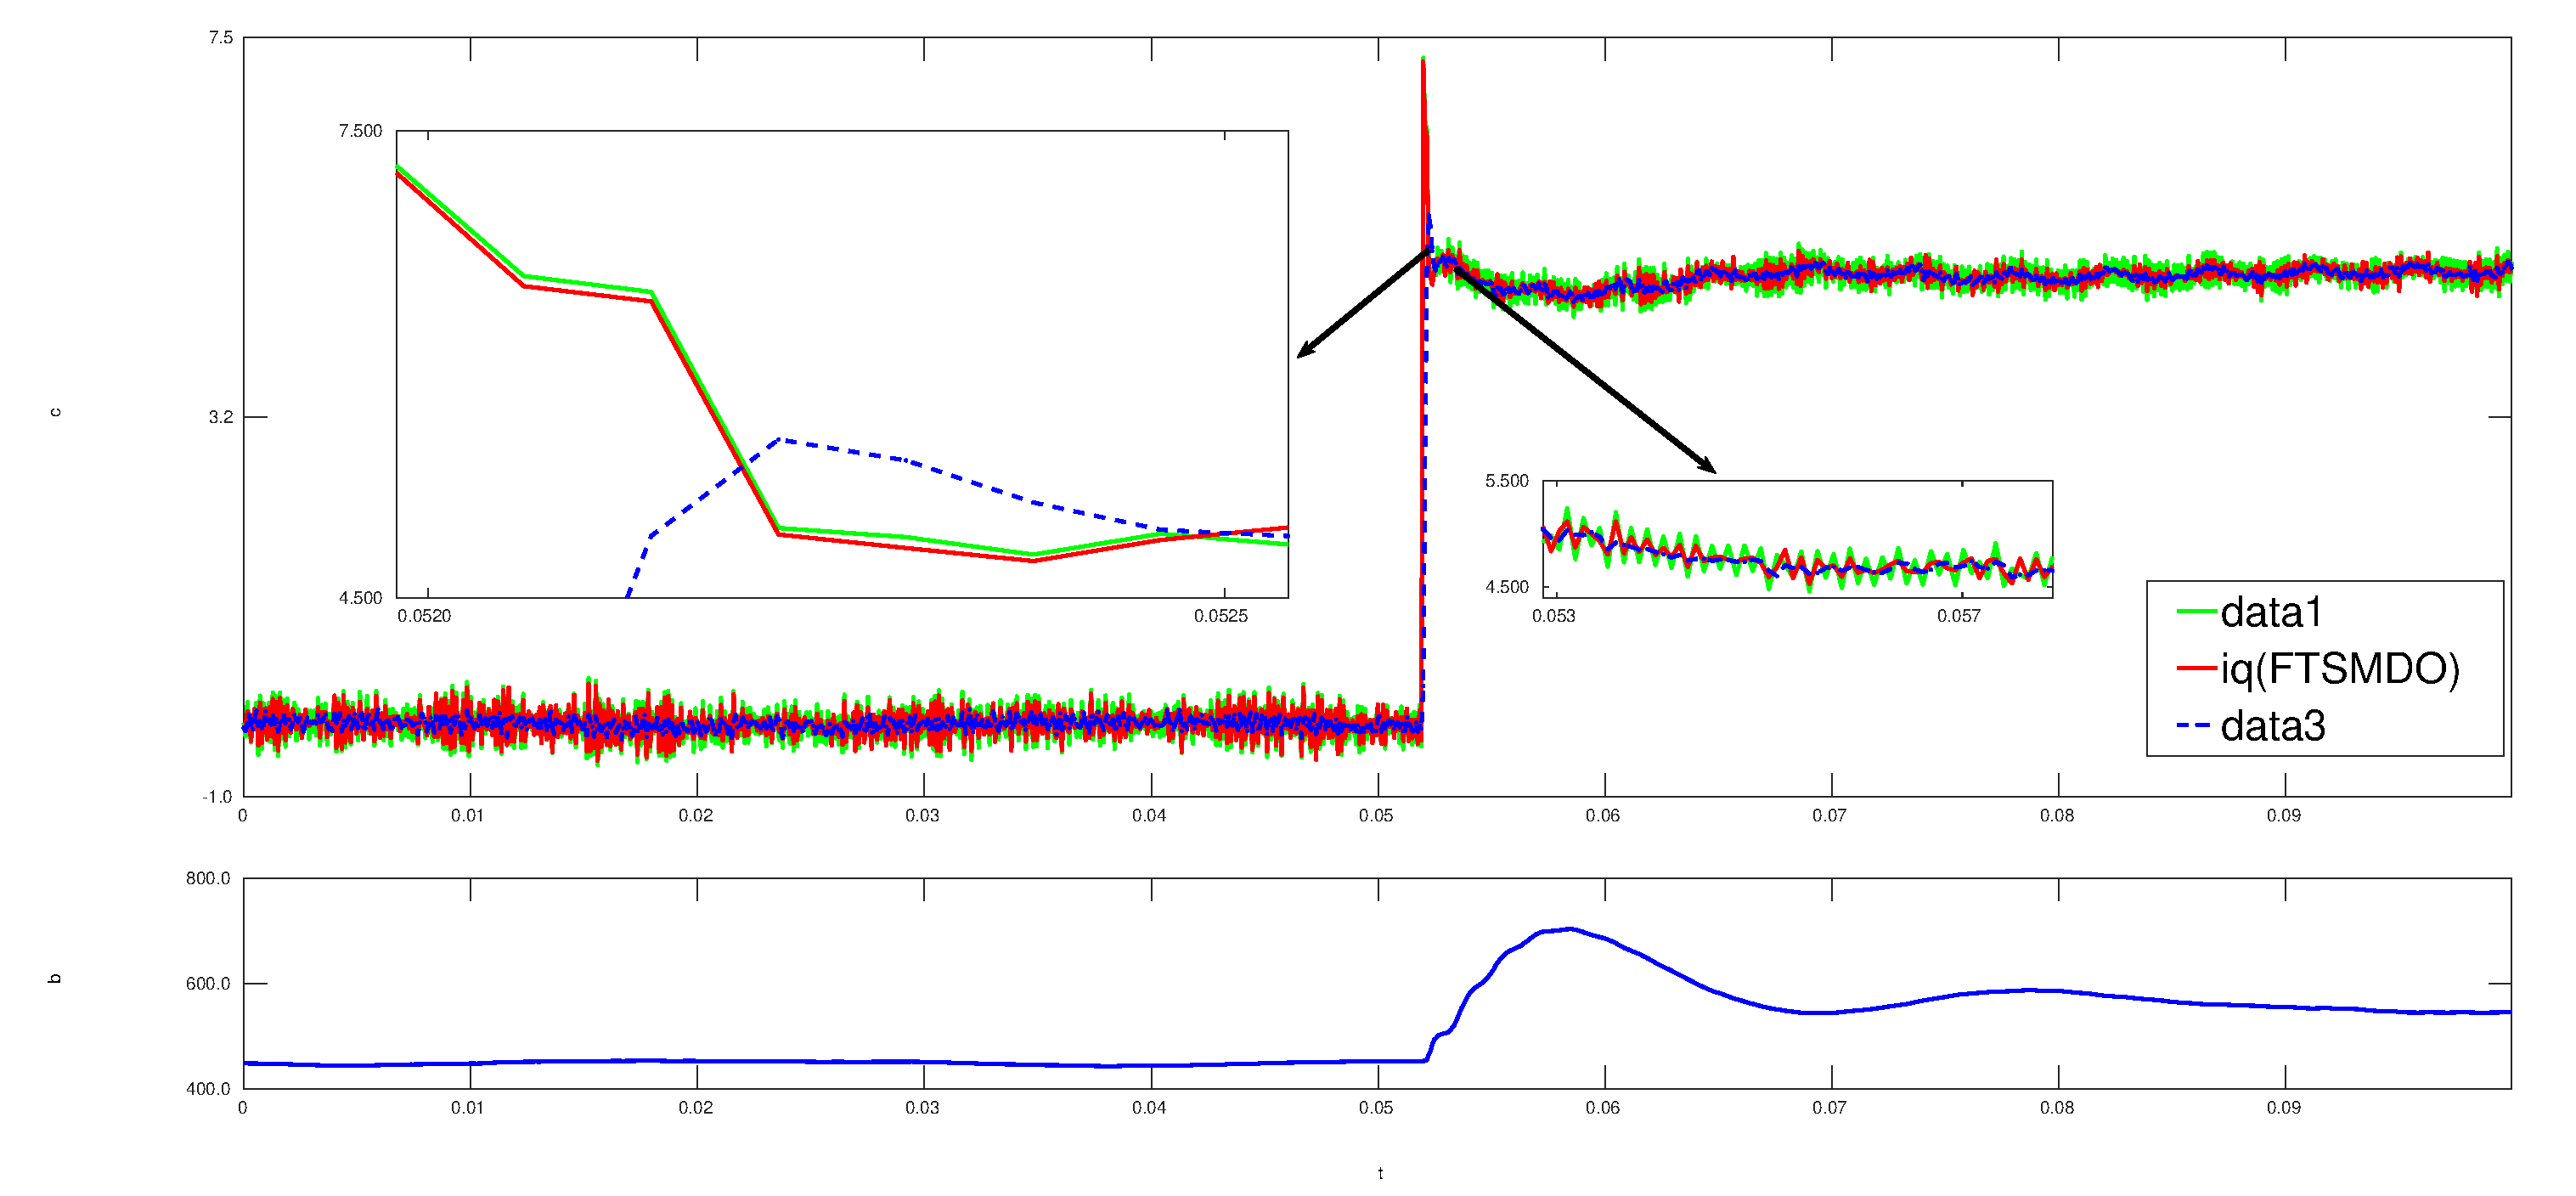
\includegraphics[width=0.50\textwidth]{./figures/current_estimate.eps}}\\
\caption{The $\hat{i}_q$ experimental results of the FTSMDO and SMDO under the $i_q$ step response test with the conventional DPCC. ($\rm 450  \; rpm$, $i_q$ alters from $\rm 0A$ to $\rm 5A$).}
\label{current_estimate}
\end{figure}


\begin{figure}[htbp]
\def\size{0.6}
\def\sizetwo{0.45}
\centering
\psfrag{0}[tc][tc][\size]{$\bm{0}$}
\psfrag{0.05}[tc][tc][\size]{$\bm{0.05}$}
\psfrag{0.15}[tc][tc][\size]{$\bm{0.15}$}
\psfrag{0.25}[tc][tc][\size]{$\bm{0.25}$}
\psfrag{0.35}[tc][tc][\size]{$\bm{0.35}$}

\psfrag{0.1}[tc][tc][\size]{$\bm{0.1}$}
\psfrag{0.2}[tc][tc][\size]{$\bm{0.2}$}
\psfrag{0.3}[tc][tc][\size]{$\bm{0.3}$}
\psfrag{0.4}[tc][tc][\size]{$\bm{0.4}$}
\psfrag{0.5}[tc][tc][\size]{$\bm{0.5}$}
\psfrag{0.6}[tc][tc][\size]{$\bm{0.6}$}
\psfrag{0.7}[tc][tc][\size]{$\bm{0.7}$}
\psfrag{0.8}[tc][tc][\size]{$\bm{0.8}$}
\psfrag{0.9}[tc][tc][\size]{$\bm{0.9}$}
\psfrag{1}[tc][tc][\size]{$\bm{1}$}
\psfrag{-4.00}[r][r][\size]{$\bm{-4}$}
\psfrag{4.00}[r][r][\size]{$\bm{4}$}
\psfrag{-4}[r][r][\size]{$\bm{-4}$}
\psfrag{4.0}[r][r][\size]{$\bm{4}$}
\psfrag{-4.0}[r][r][\size]{$\bm{-4}$}
\psfrag{4}[r][r][\size]{$\bm{4}$}
\psfrag{2.00}[r][r][\sizetwo]{$\bm{2}$}
\psfrag{0.00}[c][c][\sizetwo]{$\bm{0}$}
\psfrag{800}[r][r][\size]{$\bm{800}$}
\psfrag{400}[r][r][\size]{$\bm{400}$}
\psfrag{600}[r][r][\size]{$\bm{600}$}
\psfrag{800.0}[r][r][\size]{$\bm{800}$}
\psfrag{400.0}[r][r][\size]{$\bm{400}$}
\psfrag{600.0}[r][r][\size]{$\bm{600}$}
\psfrag{-55.0}[r][r][\size]{$\bm{-55}$}
\psfrag{-110.0}[r][r][\size]{$\bm{-110}$}

\psfrag{-120.0}[r][r][\size]{$\bm{-120}$}
\psfrag{-70.0}[r][r][\size]{$\bm{-70}$}
\psfrag{-20.0}[r][r][\size]{$\bm{-20}$}
\psfrag{-1.0}[r][r][\size]{$\bm{-1}$}
\psfrag{9.0}[r][r][\size]{$\bm{9}$}


\psfrag{0.01}[tc][tc][\size]{$\bm{0.01}$}
\psfrag{0.02}[tc][tc][\size]{$\bm{0.02}$}
\psfrag{0.03}[tc][tc][\size]{$\bm{0.03}$}

\psfrag{0.04}[tc][tc][\size]{$\bm{0.04}$}
\psfrag{0.06}[tc][tc][\size]{$\bm{0.06}$}
\psfrag{0.07}[tc][tc][\size]{$\bm{0.07}$}

\psfrag{0.08}[tc][tc][\size]{$\bm{0.08}$}
\psfrag{0.09}[tc][tc][\size]{$\bm{0.09}$}


\psfrag{-105.00}[r][r][\sizetwo]{$\bm{-105}$}
\psfrag{-111.00}[r][r][\sizetwo]{$\bm{-111}$}
\psfrag{0.208}[c][c][\sizetwo]{$\bm{0.208}$}
\psfrag{0.212}[c][c][\sizetwo]{$\bm{0.212}$}
\psfrag{4.75}[r][r][\sizetwo]{$\bm{4.75}$}
\psfrag{5.20}[r][r][\sizetwo]{$\bm{5.2}$}
\psfrag{0.000}[r][r][\sizetwo]{$\bm{0}$}
\psfrag{-110.000}[r][r][\sizetwo]{$\bm{-110}$}
\psfrag{0.0519}[tc][tc][\sizetwo]{$\bm{0.0519}$}
\psfrag{0.0523}[tc][tc][\sizetwo]{$\bm{0.0523}$}
\psfrag{-95.000}[r][r][\sizetwo]{$\bm{-95}$}
\psfrag{-110.000}[r][r][\sizetwo]{$\bm{-110}$}
\psfrag{0.060}[tc][tc][\sizetwo]{$\bm{0.06}$}
\psfrag{0.064}[tc][tc][\sizetwo]{$\bm{0.064}$}

\psfrag{data1}[l][l][\sizetwo]{$\bm{\hat{n}_q} \rm (SMDO)$}
\psfrag{nq(FTSMDO)}[l][l][\sizetwo]{$\bm{\hat{n}_q} \rm (FTSMDO)$}

\psfrag{2.0}[c][c][\sizetwo]{$\bm{2}$}
\psfrag{0.0}[c][c][\size]{$\bm{0}$}
\psfrag{0.612}[c][c][\sizetwo]{$\bm{0.612}$}
\psfrag{0.614}[l][l][\sizetwo]{$\bm{0.614}$}

\psfrag{2.00}[c][c][\sizetwo]{$\bm{2}$}
\psfrag{0.00}[c][c][\sizetwo]{$\bm{0}$}
\psfrag{0.200}[c][c][\sizetwo]{$\bm{0.2}$}
\psfrag{0.202}[l][l][\sizetwo]{$\bm{0.202}$}

\psfrag{0.70}[c][c][\sizetwo]{$\bm{0.7}$}
\psfrag{0.90}[l][l][\sizetwo]{$\bm{0.9}$}
\psfrag{1.7}[r][r][\sizetwo]{$\bm{1.7}$}
\psfrag{2.3}[r][r][\sizetwo]{$\bm{2.3}$}
\psfrag{0.300}[c][c][\sizetwo]{$\bm{0.3}$}
\psfrag{0.38}[l][l][\sizetwo]{$\bm{0.38}$}
\psfrag{0.310}[c][c][\sizetwo]{$\bm{0.31}$}
\psfrag{0.320}[c][c][\sizetwo]{$\bm{0.32}$}
\psfrag{0.39}[l][l][\sizetwo]{$\bm{0.39}$}

\psfrag{1.70}[r][r][\sizetwo]{$\bm{1.7}$}
\psfrag{2.30}[r][r][\sizetwo]{$\bm{2.3}$}


\psfrag{t}[tc][tc][\size]{$\rm \textbf{Time  \; [s]}$}
\psfrag{b}[c][c][\size]{$\bm{\omega_m}  \; \rm \textbf{[rpm]}$}
\psfrag{c}[c][c][\size]{$\bm{\hat{n}_q}  \; \rm \textbf {[A]}$}
%\psfrag{a}[c][c][\size]{$\bm{\hat{n}_q}  \; \rm \textbf {[V]}$}
%\psfrag{b}[c][c][\size]{$\bm{i_q}  \; \rm \textbf {[A]}$}
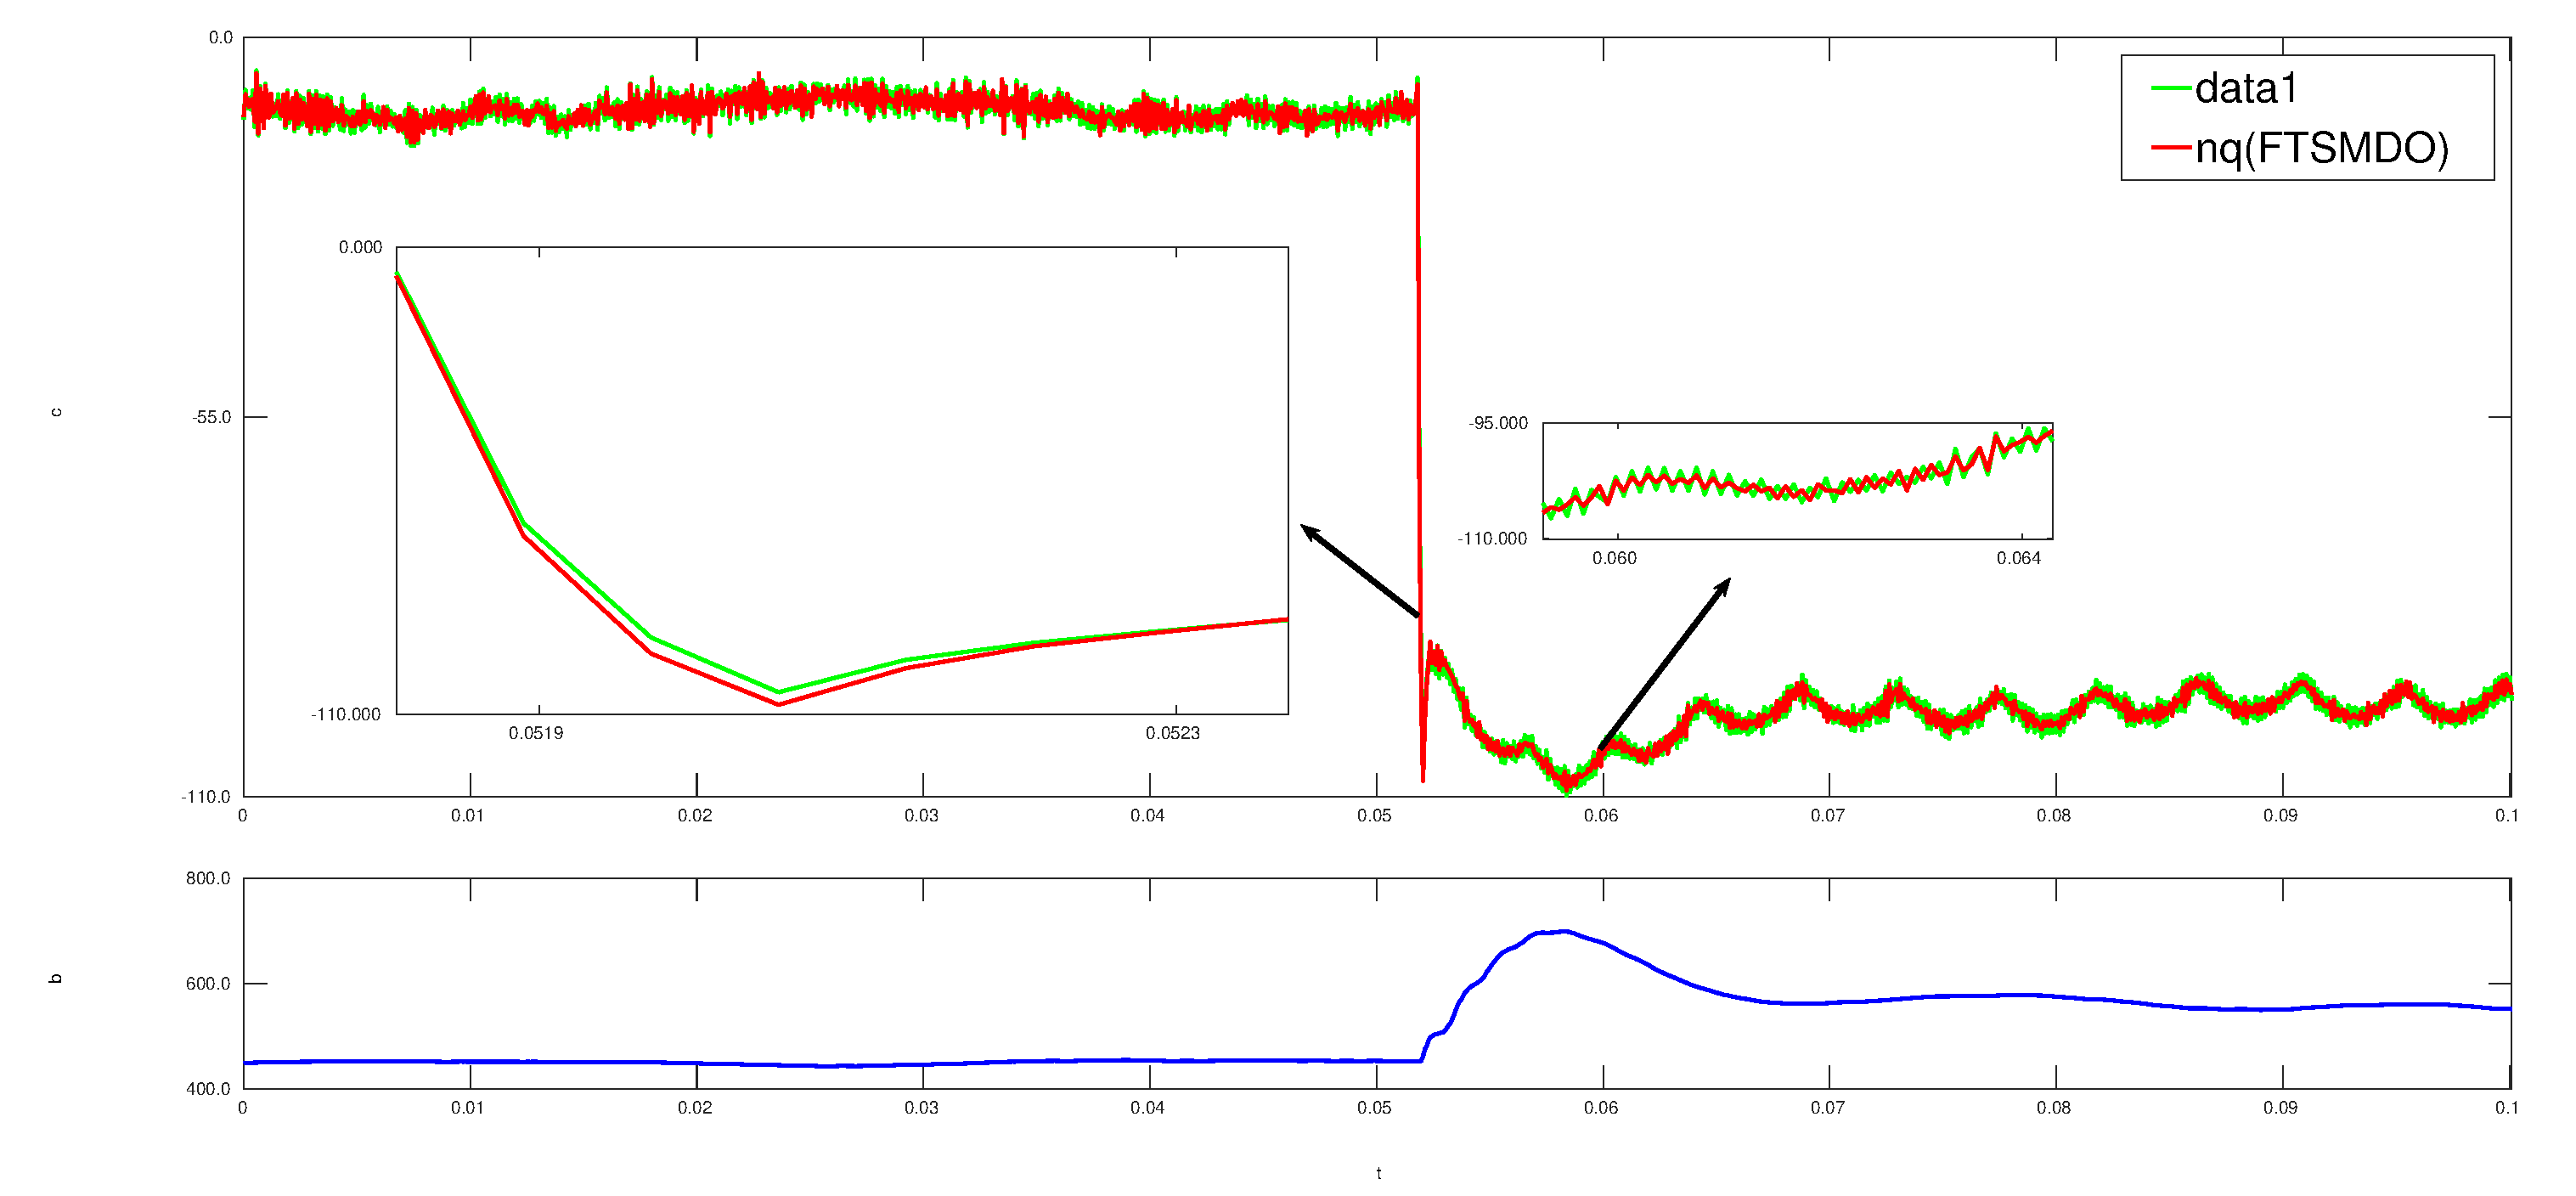
\includegraphics[width=0.50\textwidth]{./figures/disturbance_estimate.eps}}\\
\caption{The $\hat{n}_q$ experimental results of the FTSMDO and SMDO under the $i_q$ step response test with the conventional DPCC. ($\rm 450  \; rpm$, $i_q$ alters from $\rm 0A$ to $\rm 5A$).}
\label{disturbance_estimate}
\end{figure}




\subsection{$I_q$ Step Response Performance}
The $i_q$ step response performances of the conventional CCS-MPCC, EXM-CCSMPCC, SSET-CCSMPCC and MSET-CCSMPCC are evaluated in Figs. \ref{db_iqstep}, \ref{edb_iqstep}, \ref{sset_iqstep} and \ref{et_iqstep} respectively, where the $i_q^*$ is directly changed in the program and the motor speed is provided by the Micno commercial inverter. It can be seen that the SSET-CCSMPCC tracks more slowly (2ms approximately) than three other methods (within 1ms). However, both the conventional CCS-MPCC and EXM-CCSMPCC have overshoots. The overshoot of the $i_q$ is eliminated with the proposed SSET-CCSMPCC and MSET-CCSMPCC methods in the 0-2A, 2-4A, 4-0A and 0-5A step response tests. The proposed EXM-CCSMPCC and MSET-CCSMPCC have comparatable steady-state performances and the current variations are smaller than 0.28A when the $i_q$ operates at 5A. The current variations of the SSET-CCSMPCC (0.32A when the $i_q$ operates at 5A) and the conventional CCS-MPCC (0.3A when the $i_q$ operates at 5A) are larger than those of two other methods.

\begin{figure}[htbp]
\def\size{0.6}
\def\sizetwo{0.45}
\centering
\psfrag{0}[tc][tc][\size]{$\bm{0}$}
\psfrag{0.05}[tc][tc][\size]{$\bm{0.05}$}
\psfrag{0.15}[tc][tc][\size]{$\bm{0.15}$}
\psfrag{0.25}[tc][tc][\size]{$\bm{0.25}$}
\psfrag{0.35}[tc][tc][\size]{$\bm{0.35}$}
\psfrag{0.1}[tc][tc][\size]{$\bm{0.1}$}
\psfrag{0.2}[tc][tc][\size]{$\bm{0.2}$}
\psfrag{0.3}[tc][tc][\size]{$\bm{0.3}$}
\psfrag{0.4}[tc][tc][\size]{$\bm{0.4}$}
\psfrag{0.5}[tc][tc][\size]{$\bm{0.5}$}
\psfrag{0.6}[tc][tc][\size]{$\bm{0.6}$}
\psfrag{0.7}[tc][tc][\size]{$\bm{0.7}$}
\psfrag{0.8}[tc][tc][\size]{$\bm{0.8}$}
\psfrag{0.9}[tc][tc][\size]{$\bm{0.9}$}
\psfrag{1}[tc][tc][\size]{$\bm{1}$}
\psfrag{-7.00}[r][r][\size]{$\bm{-7}$}
\psfrag{7.00}[r][r][\size]{$\bm{7}$}
\psfrag{0.00}[r][r][\size]{$\bm{0}$}
\psfrag{-7.0}[r][r][\size]{$\bm{-7}$}
\psfrag{-6.0}[r][r][\size]{$\bm{-6}$}
\psfrag{6.0}[r][r][\size]{$\bm{6}$}


\psfrag{7.0}[r][r][\size]{$\bm{7}$}
\psfrag{0.0}[r][r][\size]{$\bm{0}$}
\psfrag{2.0}[r][r][\size]{$\bm{2}$}
\psfrag{700.0}[r][r][\size]{$\bm{700}$}
\psfrag{600.0}[r][r][\size]{$\bm{600}$}
\psfrag{500.0}[r][r][\size]{$\bm{500}$}
\psfrag{475.0}[r][r][\size]{$\bm{475}$}
\psfrag{250.0}[r][r][\size]{$\bm{250}$}

\psfrag{-1.00}[br][br][\sizetwo]{$\bm{-1}$}
\psfrag{6.00}[r][r][\sizetwo]{$\bm{6}$}
\psfrag{0.281}[r][r][\sizetwo]{$\bm{0.281}$}
\psfrag{0.284}[l][l][\sizetwo]{$\bm{0.284}$}

\psfrag{5.15}[r][r][\sizetwo]{$\bm{5.15}$}
\psfrag{4.85}[br][br][\sizetwo]{$\bm{4.85}$}

\psfrag{5.04}[r][r][\sizetwo]{$\bm{5.04}$}
\psfrag{4.75}[r][r][\sizetwo]{$\bm{4.75}$}
\psfrag{0.300}[c][c][\sizetwo]{$\bm{0.3}$}
\psfrag{0.350}[c][c][\sizetwo]{$\bm{0.35}$}

\psfrag{t}[tc][tc][\size]{$\rm \textbf{Time  \; [s]}$}
\psfrag{d}[c][c][\size]{$\bm{\omega_m}  \; \rm \textbf{[rpm]}$}
\psfrag{b}[c][c][\size]{$\bm{i_q}  \; \rm \textbf {[A]}$}
\psfrag{a}[c][c][\size]{$\bm{i_a}  \; \rm \textbf {[A]}$}
\psfrag{c}[c][c][\size]{$\bm{i_d}  \; \rm \textbf {[A]}$}

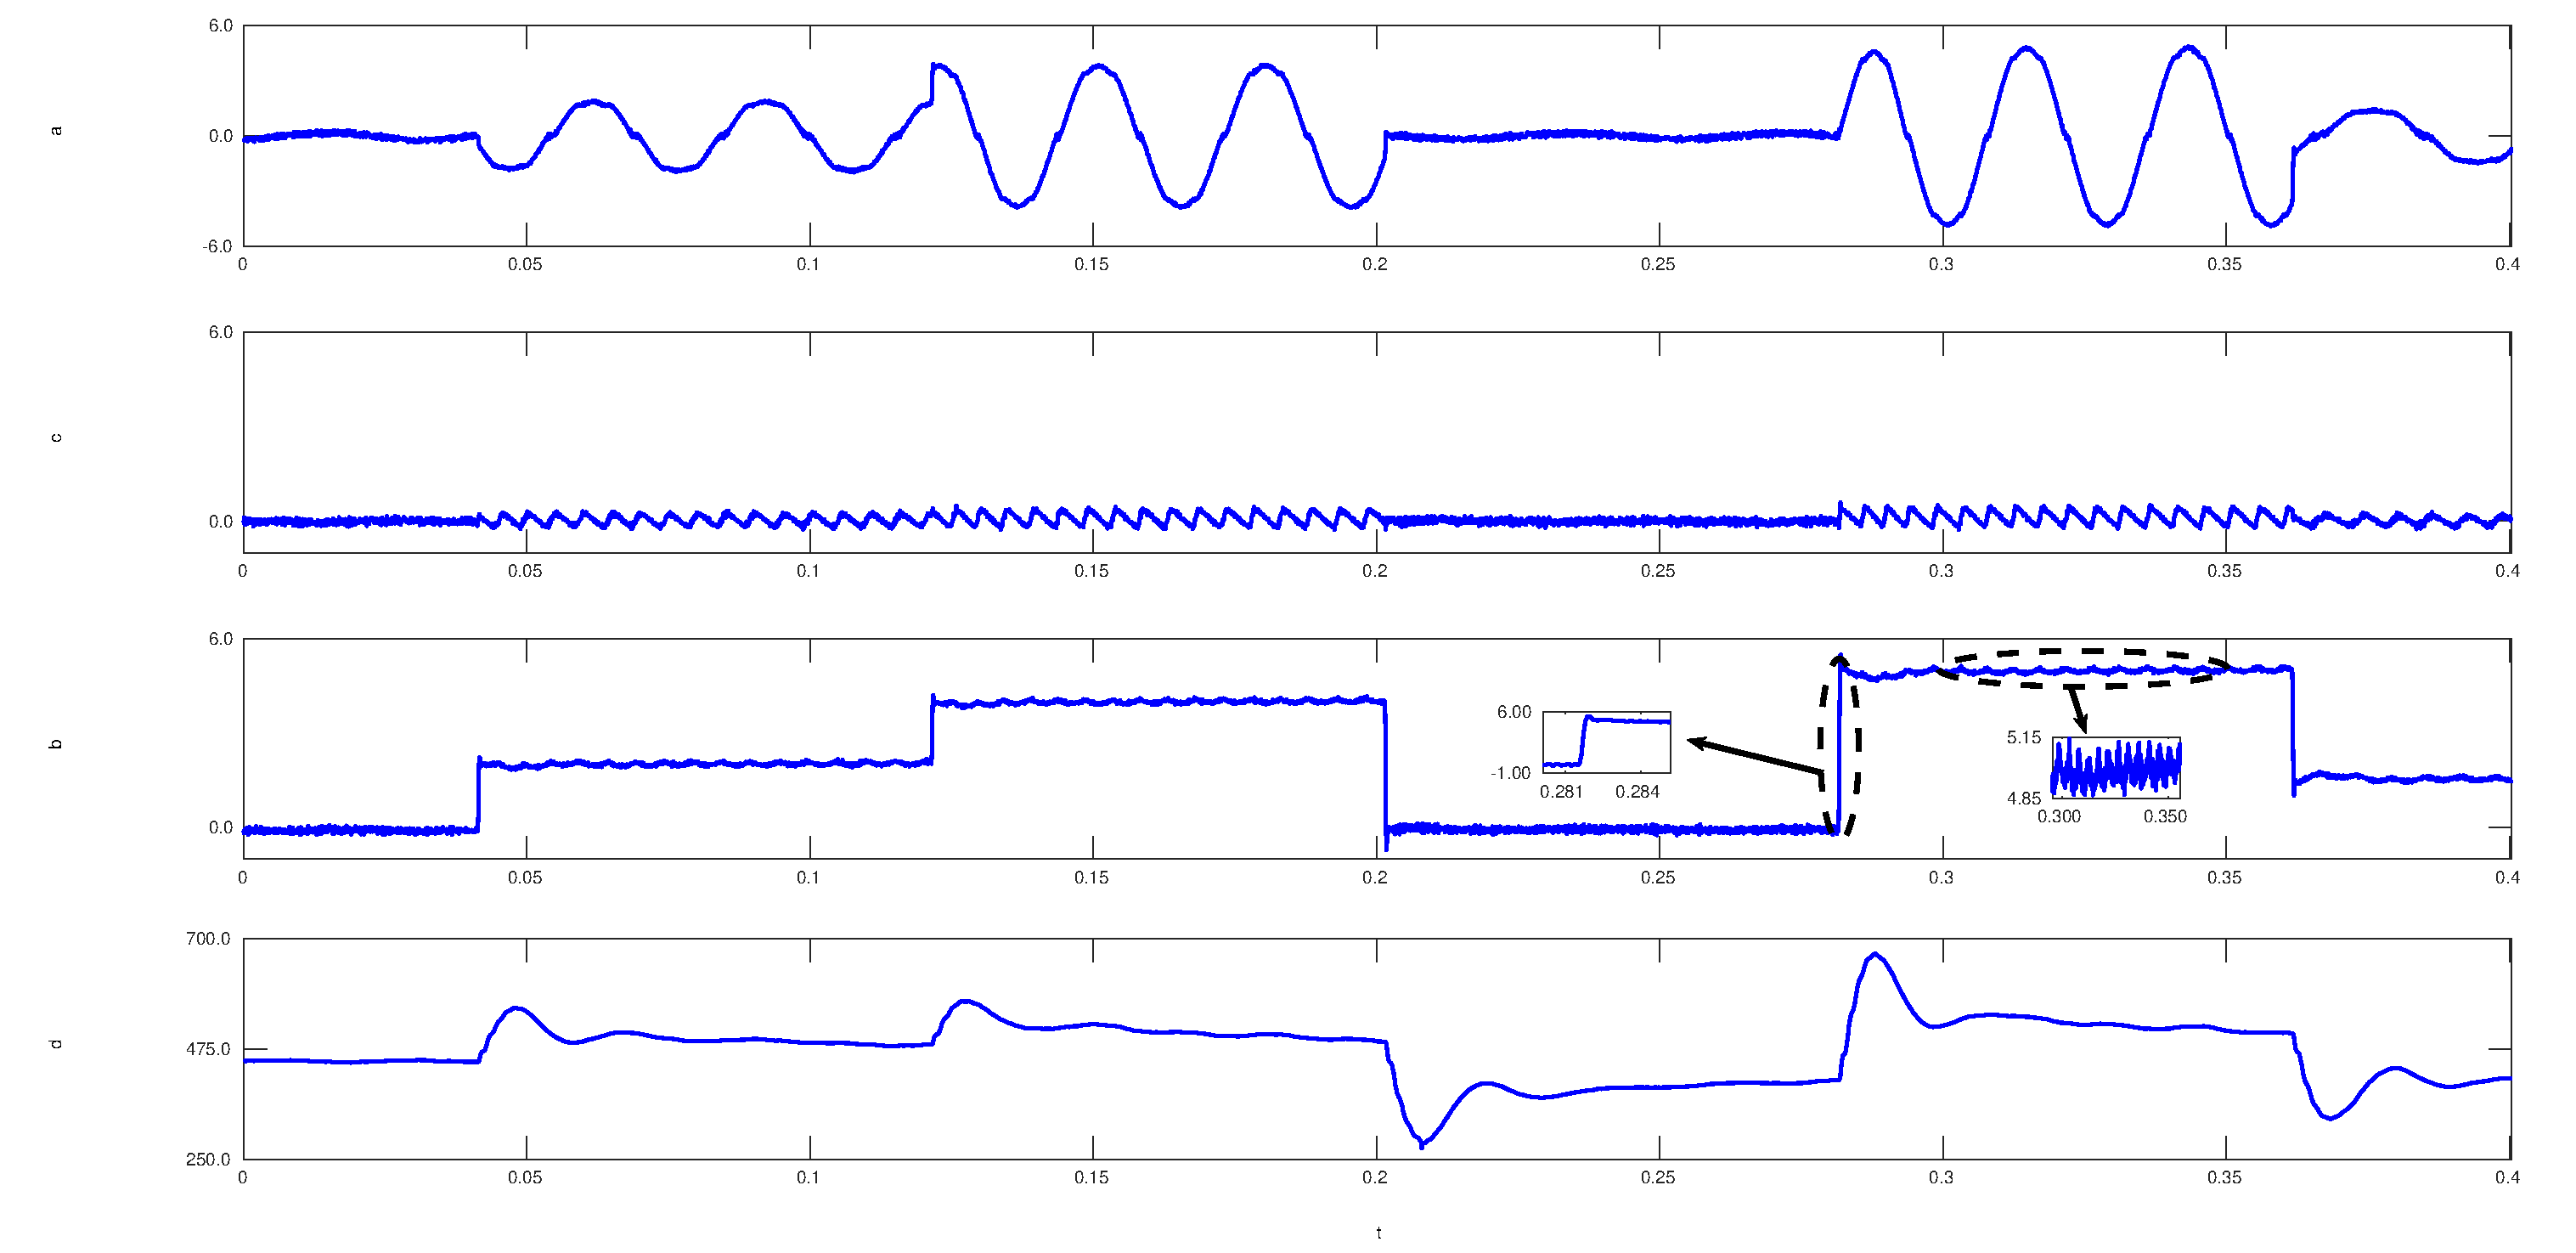
\includegraphics[width=0.50\textwidth]{./figures/db_iqstep.eps}}\\
\caption{Experimental results of the $i_q$ step response test. (With the conventional CCS-MPCC, $\rm 450  \; rpm$).}
\label{db_iqstep}
\end{figure}



\begin{figure}[htbp]
\def\size{0.6}
\def\sizetwo{0.45}
\centering
\psfrag{0}[tc][tc][\size]{$\bm{0}$}
\psfrag{0.05}[tc][tc][\size]{$\bm{0.05}$}
\psfrag{0.15}[tc][tc][\size]{$\bm{0.15}$}
\psfrag{0.25}[tc][tc][\size]{$\bm{0.25}$}
\psfrag{0.35}[tc][tc][\size]{$\bm{0.35}$}
\psfrag{0.1}[tc][tc][\size]{$\bm{0.1}$}
\psfrag{0.2}[tc][tc][\size]{$\bm{0.2}$}
\psfrag{0.3}[tc][tc][\size]{$\bm{0.3}$}
\psfrag{0.4}[tc][tc][\size]{$\bm{0.4}$}
\psfrag{0.5}[tc][tc][\size]{$\bm{0.5}$}
\psfrag{0.6}[tc][tc][\size]{$\bm{0.6}$}
\psfrag{0.7}[tc][tc][\size]{$\bm{0.7}$}
\psfrag{0.8}[tc][tc][\size]{$\bm{0.8}$}
\psfrag{0.9}[tc][tc][\size]{$\bm{0.9}$}
\psfrag{1}[tc][tc][\size]{$\bm{1}$}
\psfrag{-7.00}[r][r][\size]{$\bm{-7}$}
\psfrag{7.00}[r][r][\size]{$\bm{7}$}
\psfrag{0.00}[r][r][\size]{$\bm{0}$}
\psfrag{-7.0}[r][r][\size]{$\bm{-7}$}
\psfrag{-6.0}[r][r][\size]{$\bm{-6}$}
\psfrag{6.0}[r][r][\size]{$\bm{6}$}


\psfrag{7.0}[r][r][\size]{$\bm{7}$}
\psfrag{0.0}[r][r][\size]{$\bm{0}$}
\psfrag{2.0}[r][r][\size]{$\bm{2}$}
\psfrag{700.0}[r][r][\size]{$\bm{700}$}
\psfrag{600.0}[r][r][\size]{$\bm{600}$}
\psfrag{500.0}[r][r][\size]{$\bm{500}$}
\psfrag{475.0}[r][r][\size]{$\bm{475}$}
\psfrag{250.0}[r][r][\size]{$\bm{250}$}

\psfrag{-1.00}[br][br][\sizetwo]{$\bm{-1}$}
\psfrag{6.00}[r][r][\sizetwo]{$\bm{6}$}
\psfrag{0.281}[r][r][\sizetwo]{$\bm{0.281}$}
\psfrag{0.284}[l][l][\sizetwo]{$\bm{0.284}$}

\psfrag{5.14}[r][r][\sizetwo]{$\bm{5.14}$}
\psfrag{4.86}[br][br][\sizetwo]{$\bm{4.86}$}
\psfrag{0.300}[c][c][\sizetwo]{$\bm{0.3}$}
\psfrag{0.350}[c][c][\sizetwo]{$\bm{0.35}$}

\psfrag{t}[tc][tc][\size]{$\rm \textbf{Time  \; [s]}$}
\psfrag{d}[c][c][\size]{$\bm{\omega_m}  \; \rm \textbf{[rpm]}$}
\psfrag{b}[c][c][\size]{$\bm{i_q}  \; \rm \textbf {[A]}$}
\psfrag{a}[c][c][\size]{$\bm{i_a}  \; \rm \textbf {[A]}$}
\psfrag{c}[c][c][\size]{$\bm{i_d}  \; \rm \textbf {[A]}$}

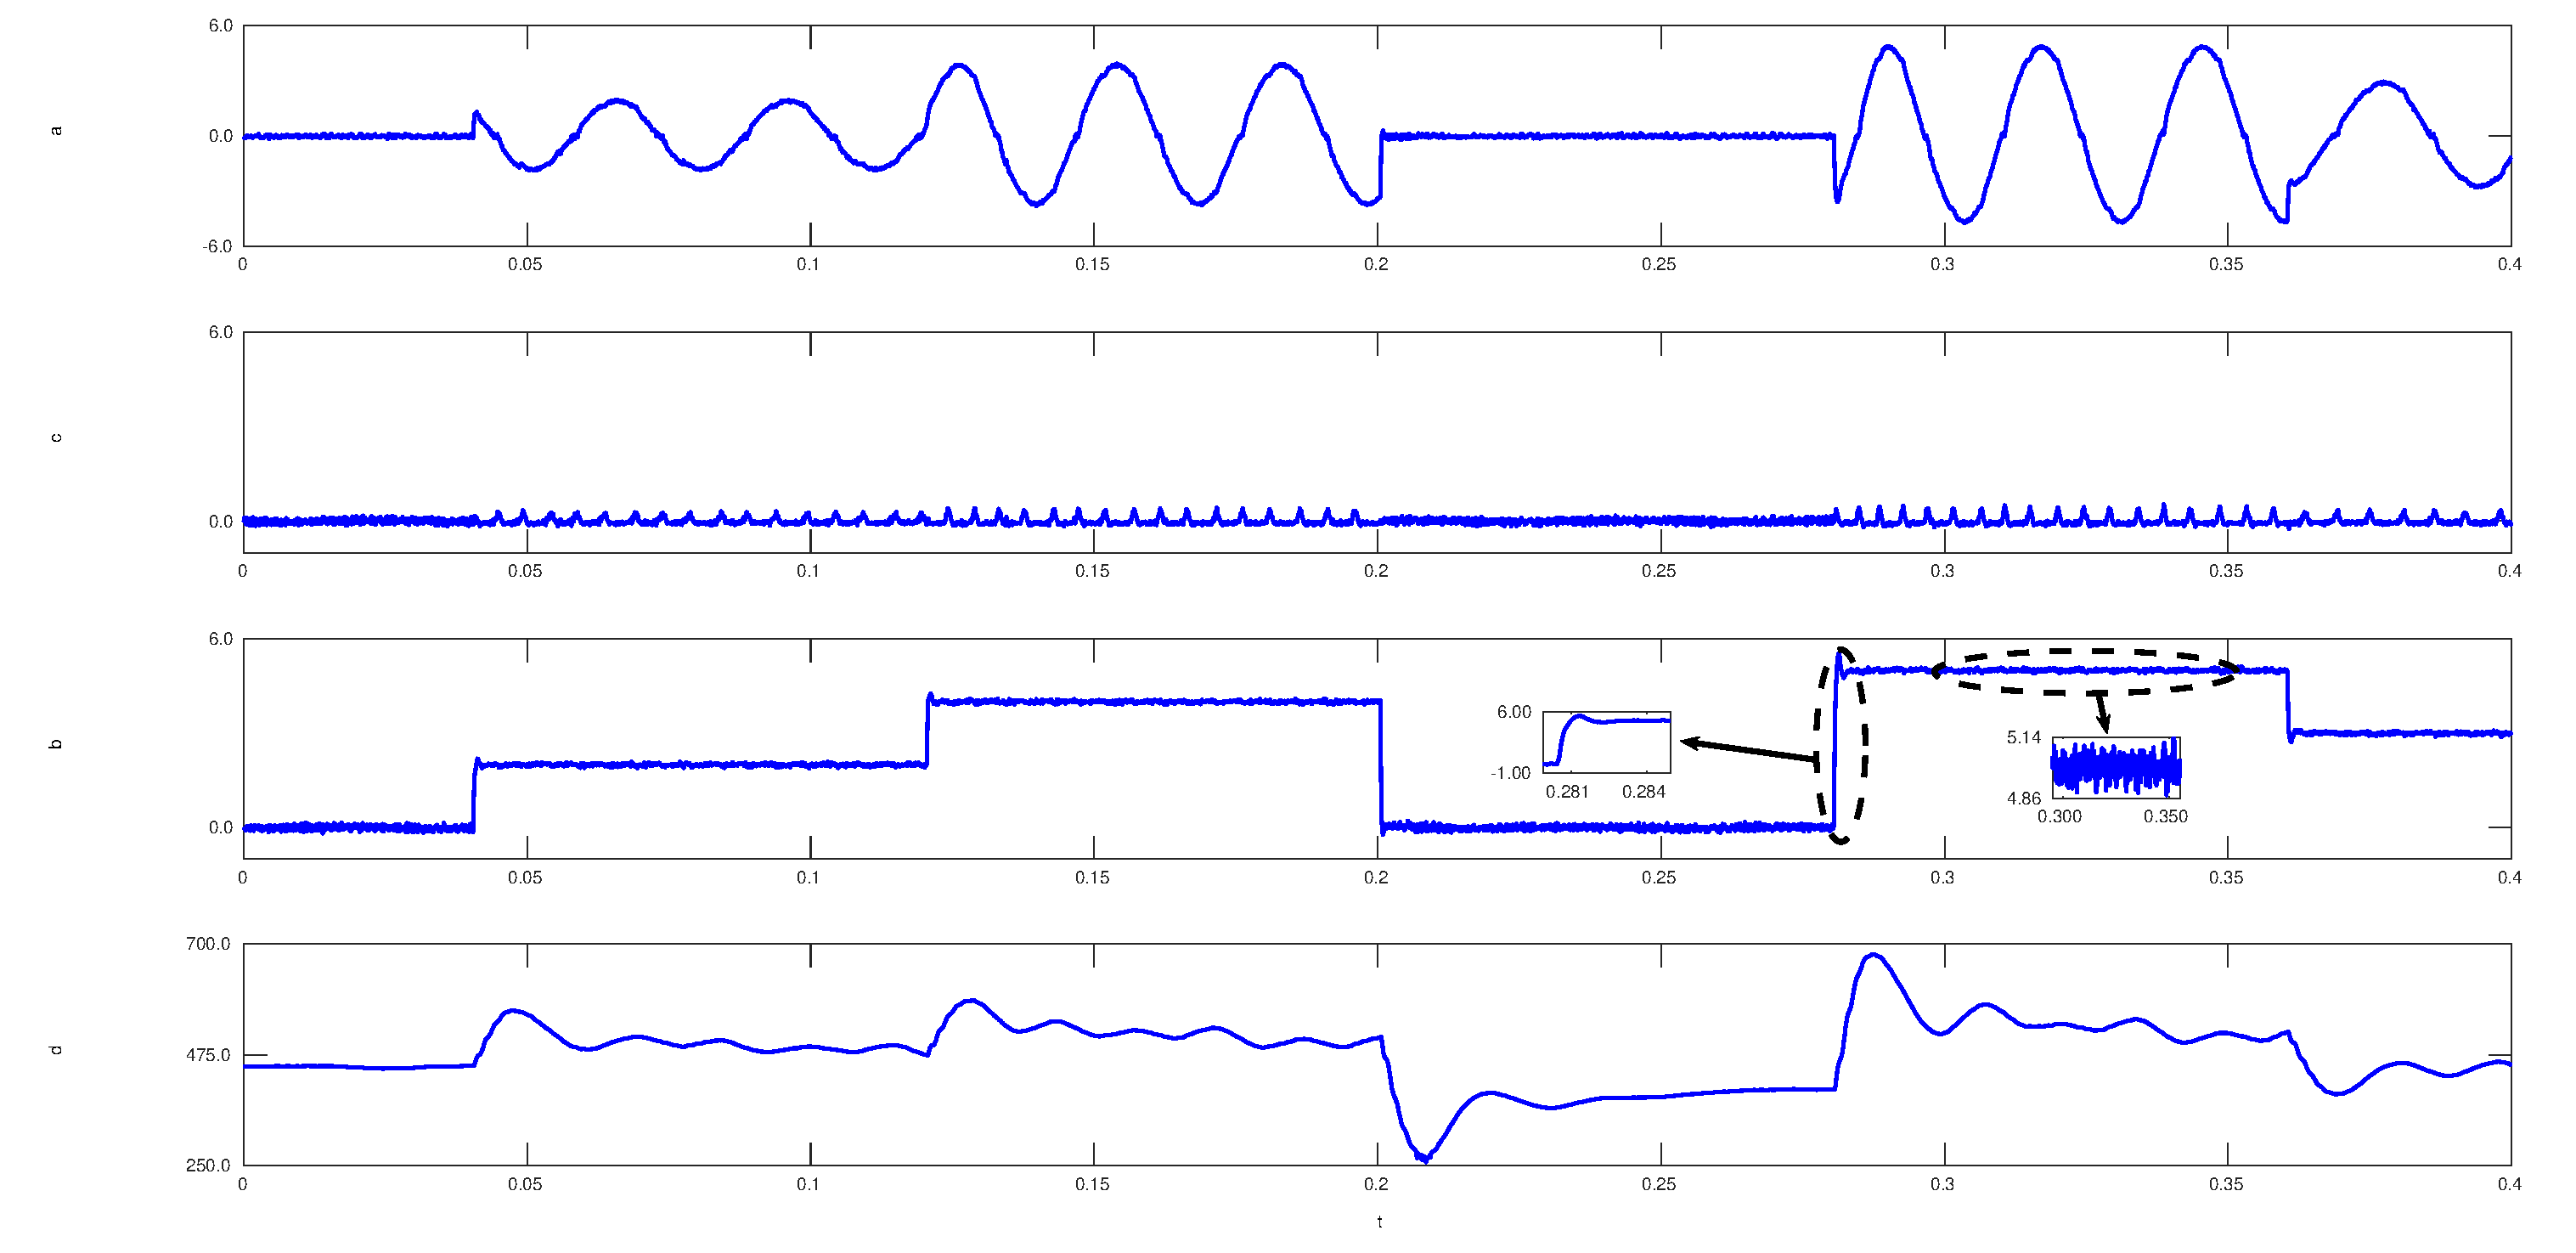
\includegraphics[width=0.50\textwidth]{./figures/edb_iqstep.eps}}\\
\caption{Experimental results of the $i_q$ step response test. (With the EXM-CCSMPCC, $\rm 450  \; rpm$).}
\label{edb_iqstep}
\end{figure}

\begin{figure}[htbp]
\def\size{0.6}
\def\sizetwo{0.45}
\centering
\psfrag{0}[tc][tc][\size]{$\bm{0}$}
\psfrag{0.05}[tc][tc][\size]{$\bm{0.05}$}
\psfrag{0.15}[tc][tc][\size]{$\bm{0.15}$}
\psfrag{0.25}[tc][tc][\size]{$\bm{0.25}$}
\psfrag{0.35}[tc][tc][\size]{$\bm{0.35}$}
\psfrag{0.1}[tc][tc][\size]{$\bm{0.1}$}
\psfrag{0.2}[tc][tc][\size]{$\bm{0.2}$}
\psfrag{0.3}[tc][tc][\size]{$\bm{0.3}$}
\psfrag{0.4}[tc][tc][\size]{$\bm{0.4}$}
\psfrag{0.5}[tc][tc][\size]{$\bm{0.5}$}
\psfrag{0.6}[tc][tc][\size]{$\bm{0.6}$}
\psfrag{0.7}[tc][tc][\size]{$\bm{0.7}$}
\psfrag{0.8}[tc][tc][\size]{$\bm{0.8}$}
\psfrag{0.9}[tc][tc][\size]{$\bm{0.9}$}
\psfrag{1}[tc][tc][\size]{$\bm{1}$}
\psfrag{-7.00}[r][r][\size]{$\bm{-7}$}
\psfrag{7.00}[r][r][\size]{$\bm{7}$}
\psfrag{0.00}[r][r][\size]{$\bm{0}$}
\psfrag{-7.0}[r][r][\size]{$\bm{-7}$}
\psfrag{-6.0}[r][r][\size]{$\bm{-6}$}
\psfrag{6.0}[r][r][\size]{$\bm{6}$}


\psfrag{7.0}[r][r][\size]{$\bm{7}$}
\psfrag{0.0}[r][r][\size]{$\bm{0}$}
\psfrag{2.0}[r][r][\size]{$\bm{2}$}
\psfrag{700.0}[r][r][\size]{$\bm{700}$}
\psfrag{600.0}[r][r][\size]{$\bm{600}$}
\psfrag{500.0}[r][r][\size]{$\bm{500}$}
\psfrag{475.0}[r][r][\size]{$\bm{475}$}
\psfrag{250.0}[r][r][\size]{$\bm{250}$}

\psfrag{-1.00}[r][r][\sizetwo]{$\bm{-1}$}
\psfrag{6.00}[r][r][\sizetwo]{$\bm{6}$}
\psfrag{0.281}[r][r][\sizetwo]{$\bm{0.281}$}
\psfrag{0.284}[l][l][\sizetwo]{$\bm{0.284}$}

\psfrag{5.16}[r][r][\sizetwo]{$\bm{5.16}$}
\psfrag{4.84}[r][r][\sizetwo]{$\bm{4.84}$}
\psfrag{0.300}[c][c][\sizetwo]{$\bm{0.3}$}
\psfrag{0.350}[c][c][\sizetwo]{$\bm{0.35}$}

\psfrag{t}[tc][tc][\size]{$\rm \textbf{Time  \; [s]}$}
\psfrag{d}[c][c][\size]{$\bm{\omega_m}  \; \rm \textbf{[rpm]}$}
\psfrag{b}[c][c][\size]{$\bm{i_q}  \; \rm \textbf {[A]}$}
\psfrag{a}[c][c][\size]{$\bm{i_a}  \; \rm \textbf {[A]}$}
\psfrag{c}[c][c][\size]{$\bm{i_d}  \; \rm \textbf {[A]}$}

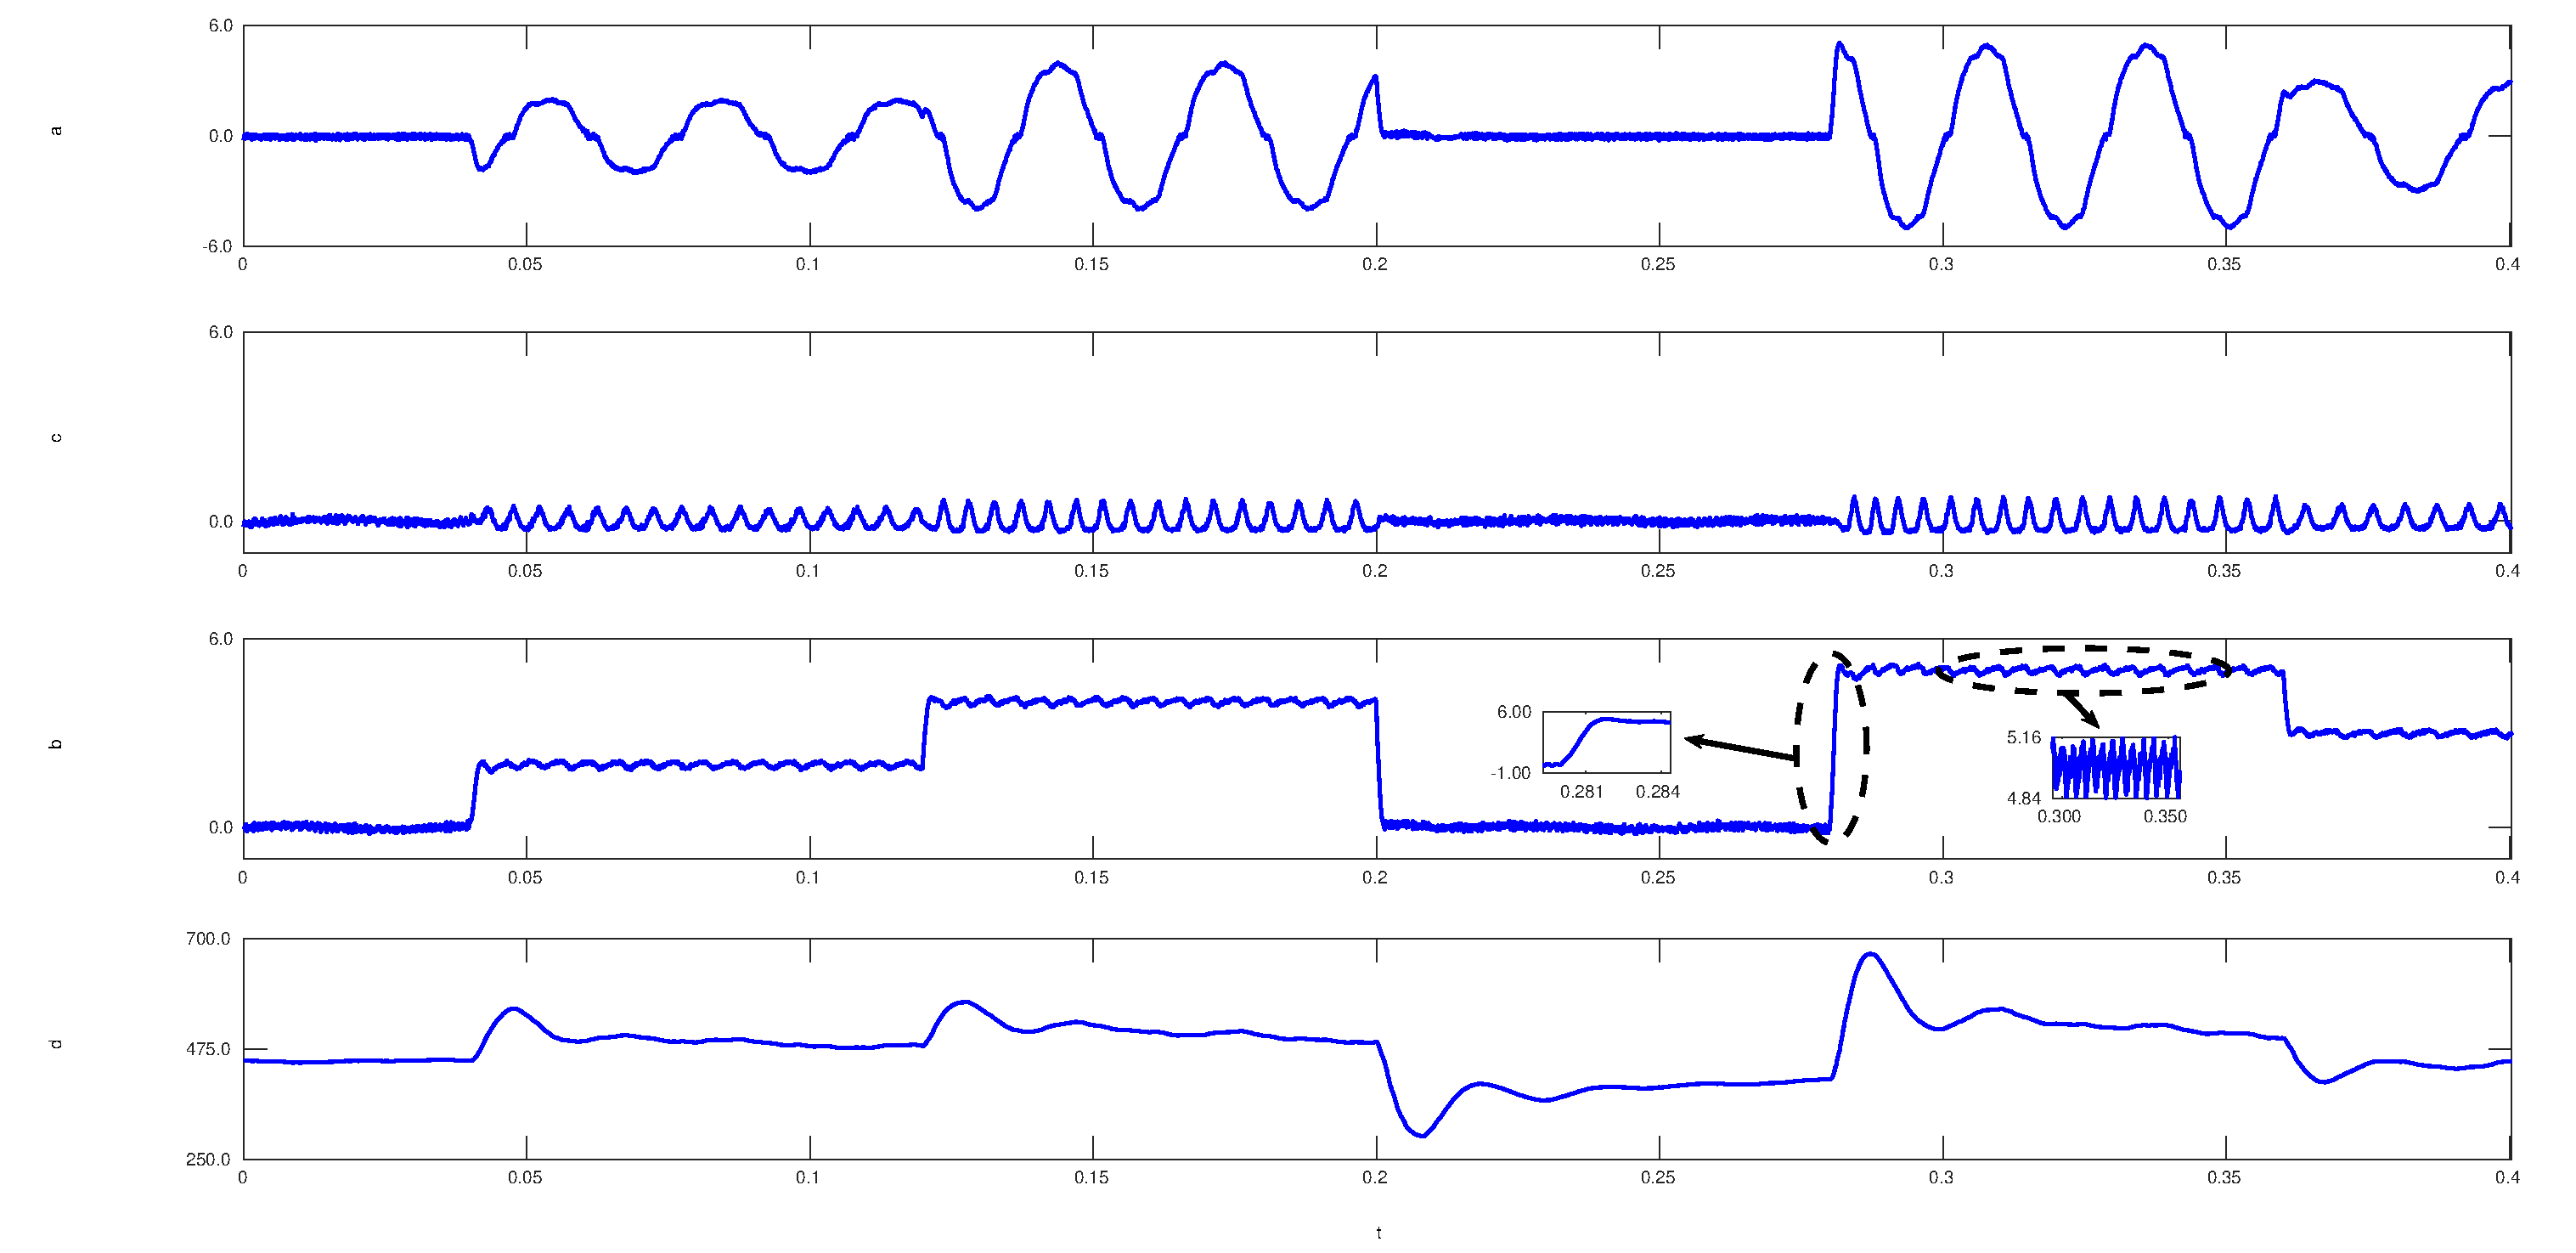
\includegraphics[width=0.50\textwidth]{./figures/sset_iqstep.eps}}\\
\caption{Experimental results of the $i_q$ step response test. (With the SSET-CCSMPCC, $\rm 450  \; rpm$).}
\label{sset_iqstep}
\end{figure}


\begin{figure}[htbp]
\def\size{0.6}
\def\sizetwo{0.45}
\centering
\psfrag{0}[tc][tc][\size]{$\bm{0}$}
\psfrag{0.05}[tc][tc][\size]{$\bm{0.05}$}
\psfrag{0.15}[tc][tc][\size]{$\bm{0.15}$}
\psfrag{0.25}[tc][tc][\size]{$\bm{0.25}$}
\psfrag{0.35}[tc][tc][\size]{$\bm{0.35}$}
\psfrag{0.1}[tc][tc][\size]{$\bm{0.1}$}
\psfrag{0.2}[tc][tc][\size]{$\bm{0.2}$}
\psfrag{0.3}[tc][tc][\size]{$\bm{0.3}$}
\psfrag{0.4}[tc][tc][\size]{$\bm{0.4}$}
\psfrag{0.5}[tc][tc][\size]{$\bm{0.5}$}
\psfrag{0.6}[tc][tc][\size]{$\bm{0.6}$}
\psfrag{0.7}[tc][tc][\size]{$\bm{0.7}$}
\psfrag{0.8}[tc][tc][\size]{$\bm{0.8}$}
\psfrag{0.9}[tc][tc][\size]{$\bm{0.9}$}
\psfrag{1}[tc][tc][\size]{$\bm{1}$}
\psfrag{-7.00}[r][r][\size]{$\bm{-7}$}
\psfrag{7.00}[r][r][\size]{$\bm{7}$}
\psfrag{0.00}[r][r][\size]{$\bm{0}$}
\psfrag{-7.0}[r][r][\size]{$\bm{-7}$}
\psfrag{-6.0}[r][r][\size]{$\bm{-6}$}
\psfrag{6.0}[r][r][\size]{$\bm{6}$}


\psfrag{7.0}[r][r][\size]{$\bm{7}$}
\psfrag{0.0}[r][r][\size]{$\bm{0}$}
\psfrag{2.0}[r][r][\size]{$\bm{2}$}
\psfrag{700.0}[r][r][\size]{$\bm{700}$}
\psfrag{600.0}[r][r][\size]{$\bm{600}$}
\psfrag{500.0}[r][r][\size]{$\bm{500}$}
\psfrag{475.0}[r][r][\size]{$\bm{475}$}
\psfrag{250.0}[r][r][\size]{$\bm{250}$}

\psfrag{-1.00}[r][r][\sizetwo]{$\bm{-1}$}
\psfrag{6.00}[r][r][\sizetwo]{$\bm{6}$}
\psfrag{0.281}[r][r][\sizetwo]{$\bm{0.281}$}
\psfrag{0.284}[l][l][\sizetwo]{$\bm{0.284}$}

\psfrag{5.14}[r][r][\sizetwo]{$\bm{5.14}$}
\psfrag{4.86}[r][r][\sizetwo]{$\bm{4.86}$}
\psfrag{0.300}[c][c][\sizetwo]{$\bm{0.3}$}
\psfrag{0.350}[c][c][\sizetwo]{$\bm{0.35}$}

\psfrag{t}[tc][tc][\size]{$\rm \textbf{Time  \; [s]}$}
\psfrag{d}[c][c][\size]{$\bm{\omega_m}  \; \rm \textbf{[rpm]}$}
\psfrag{b}[c][c][\size]{$\bm{i_q}  \; \rm \textbf {[A]}$}
\psfrag{a}[c][c][\size]{$\bm{i_a}  \; \rm \textbf {[A]}$}
\psfrag{c}[c][c][\size]{$\bm{i_d}  \; \rm \textbf {[A]}$}

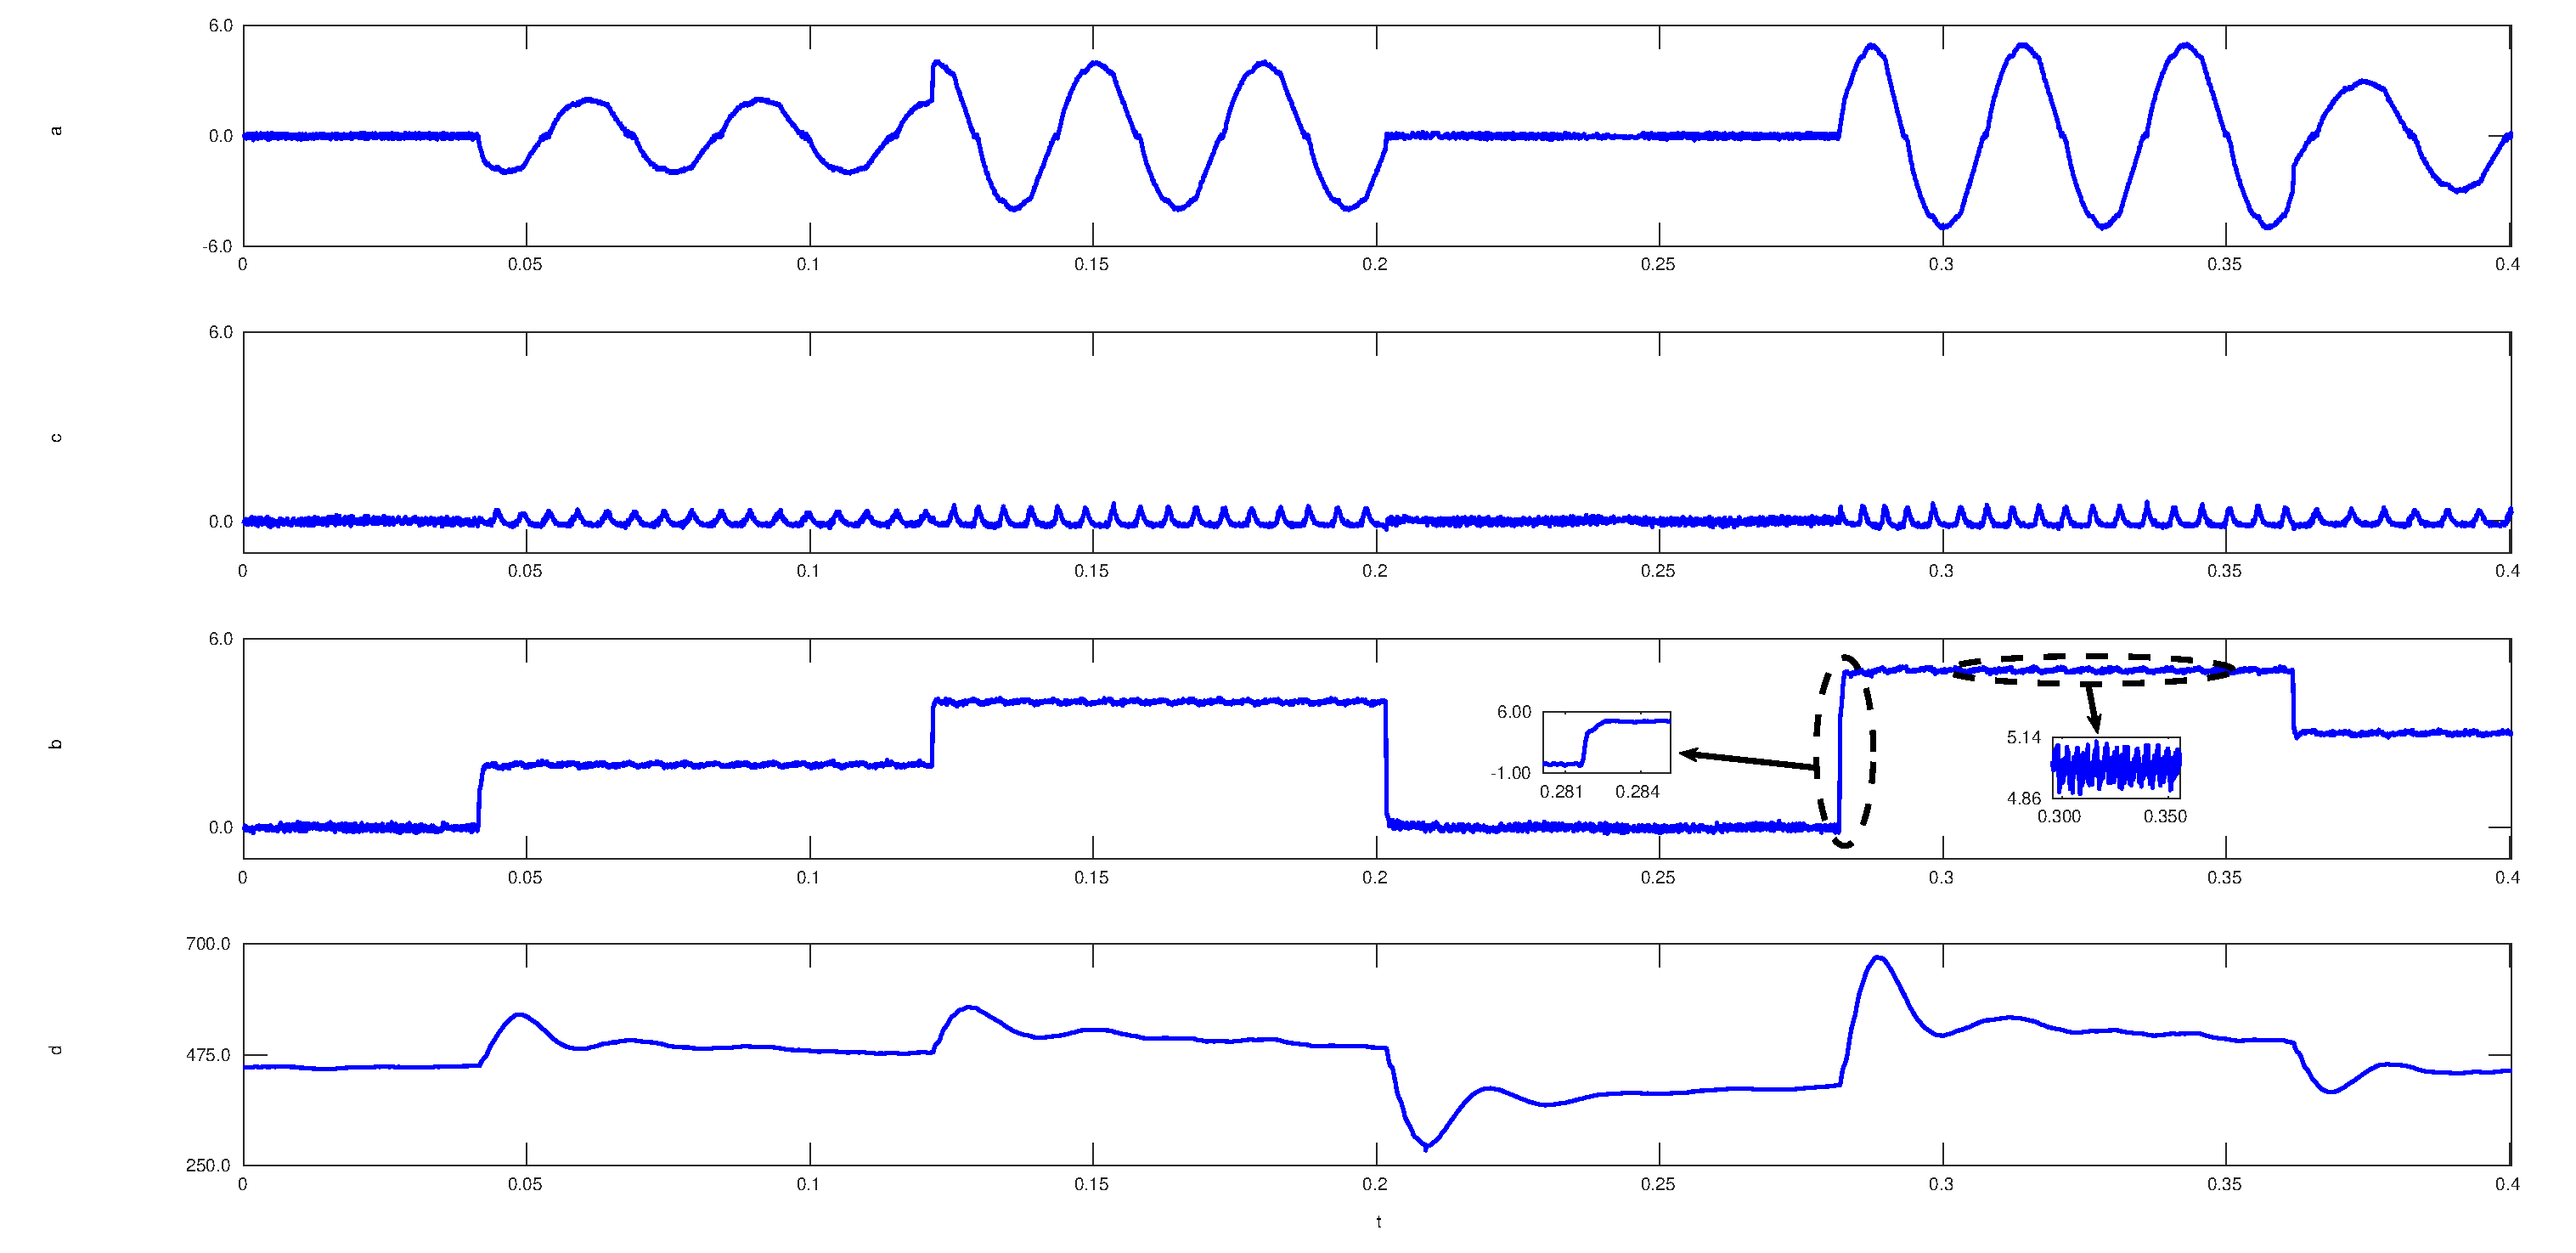
\includegraphics[width=0.50\textwidth]{./figures/et_iqstep.eps}}\\
\caption{Experimental results of the $i_q$ step response test. (With the MSET-CCSMPCC, $\rm 450  \; rpm$).}
\label{et_iqstep}
\end{figure}


\subsection{Parameter Sensitivity Evaluation}
From (\ref{eq:improved_ccsmpc}) and (\ref{eq:u_dq}), the proposed EXM-CCSMPCC and MSET-CCSMPCC are only affected by the stator inductance, while the conventional CCS-MPCC is influenced by the stator inductance, stator resistance and permanent magnet flux linkage. Fig. \ref{L_robust_db} shows the experimental results of the conventional CCS-MPCC, where the feedback $i_q$ decreases with the decreasing of the stator inductance. Figs. \ref{L_robust_edb} and \ref{L_robust_et} compare the steady-state performances of the proposed EXM-CCSMPCC and MSET-CCSMPCC under the stator inductance variation. In the whole range of the inductance variation, the $i_q$ keeps the average value of 5A with both methods. The stator inductance jumps to 9mH at 0.05s, the $i_q$ of the EXM-CCSMPCC has a large chatter for the later 0.1s, while that of the MSET-CCSMPCC first jumps to 7A but returns to 5A fast. When the stator inductance deceases from 6mH to 2.62mH, the $i_q$ variations of both methods are within 0.28A. When the inductance deceases from 2.62mH to 0.5mH, the $i_q$ ripples increase, but the $i_q$ ripples of the MSET-CCSMPCC increase more rapidly than that of the EXM-CCSMPCC.


\begin{figure}[htbp]
\def\size{0.6}
\def\sizetwo{0.45}
\centering
\psfrag{0}[tc][tc][\size]{$\bm{0}$}
\psfrag{0.5}[tc][tc][\size]{$\bm{0.5}$}
\psfrag{1}[tc][tc][\size]{$\bm{1}$}
\psfrag{1.5}[tc][tc][\size]{$\bm{1.5}$}
\psfrag{2}[tc][tc][\size]{$\bm{2}$}
\psfrag{2.5}[tc][tc][\size]{$\bm{2.5}$}
\psfrag{3}[tc][tc][\size]{$\bm{3}$}

\psfrag{0.0}[r][r][\size]{$\bm{0}$}
\psfrag{6.0}[r][r][\size]{$\bm{6}$}
\psfrag{3.0}[r][r][\size]{$\bm{3}$}
\psfrag{-6.0}[r][r][\size]{$\bm{-6}$}
\psfrag{7.0}[r][r][\size]{$\bm{7}$}
\psfrag{-7.0}[r][r][\size]{$\bm{-7}$}
\psfrag{10.0}[r][r][\size]{$\bm{10}$}
\psfrag{5.0}[r][r][\size]{$\bm{5}$}
\psfrag{-1.0}[r][r][\size]{$\bm{-1}$}

\psfrag{500.0}[r][r][\size]{$\bm{500}$}
\psfrag{400.0}[r][r][\size]{$\bm{400}$}
\psfrag{450.0}[r][r][\size]{$\bm{450}$}


\psfrag{-1.00}[r][r][\size]{$\bm{-1}$}
\psfrag{0.00}[r][r][\size]{$\bm{0}$}
\psfrag{1.00}[r][r][\size]{$\bm{1}$}
\psfrag{7.00}[r][r][\size]{$\bm{7}$}
\psfrag{3.50}[r][r][\size]{$\bm{3.5}$}


\psfrag{70}[r][r][\size]{$\bm{70}$}
\psfrag{80}[r][r][\size]{$\bm{80}$}
\psfrag{75}[r][r][\size]{$\bm{75}$}

\psfrag{t}[tc][tc][\size]{$\rm \textbf{Time  \; [s]}$}
\psfrag{d}[c][c][\size]{$\bm{\omega_m}  \; \rm \textbf{[rpm]}$}
\psfrag{b}[c][c][\size]{$\bm{i_q}  \; \rm \textbf {[A]}$}
\psfrag{a}[c][c][\size]{$\bm{i_a}  \; \rm \textbf {[A]}$}
\psfrag{c}[c][c][\size]{$\bm{i_d}  \; \rm \textbf {[A]}$}
\psfrag{c}[c][c][\size]{$\bm{L}  \; \rm \textbf  {[mH]}}$}
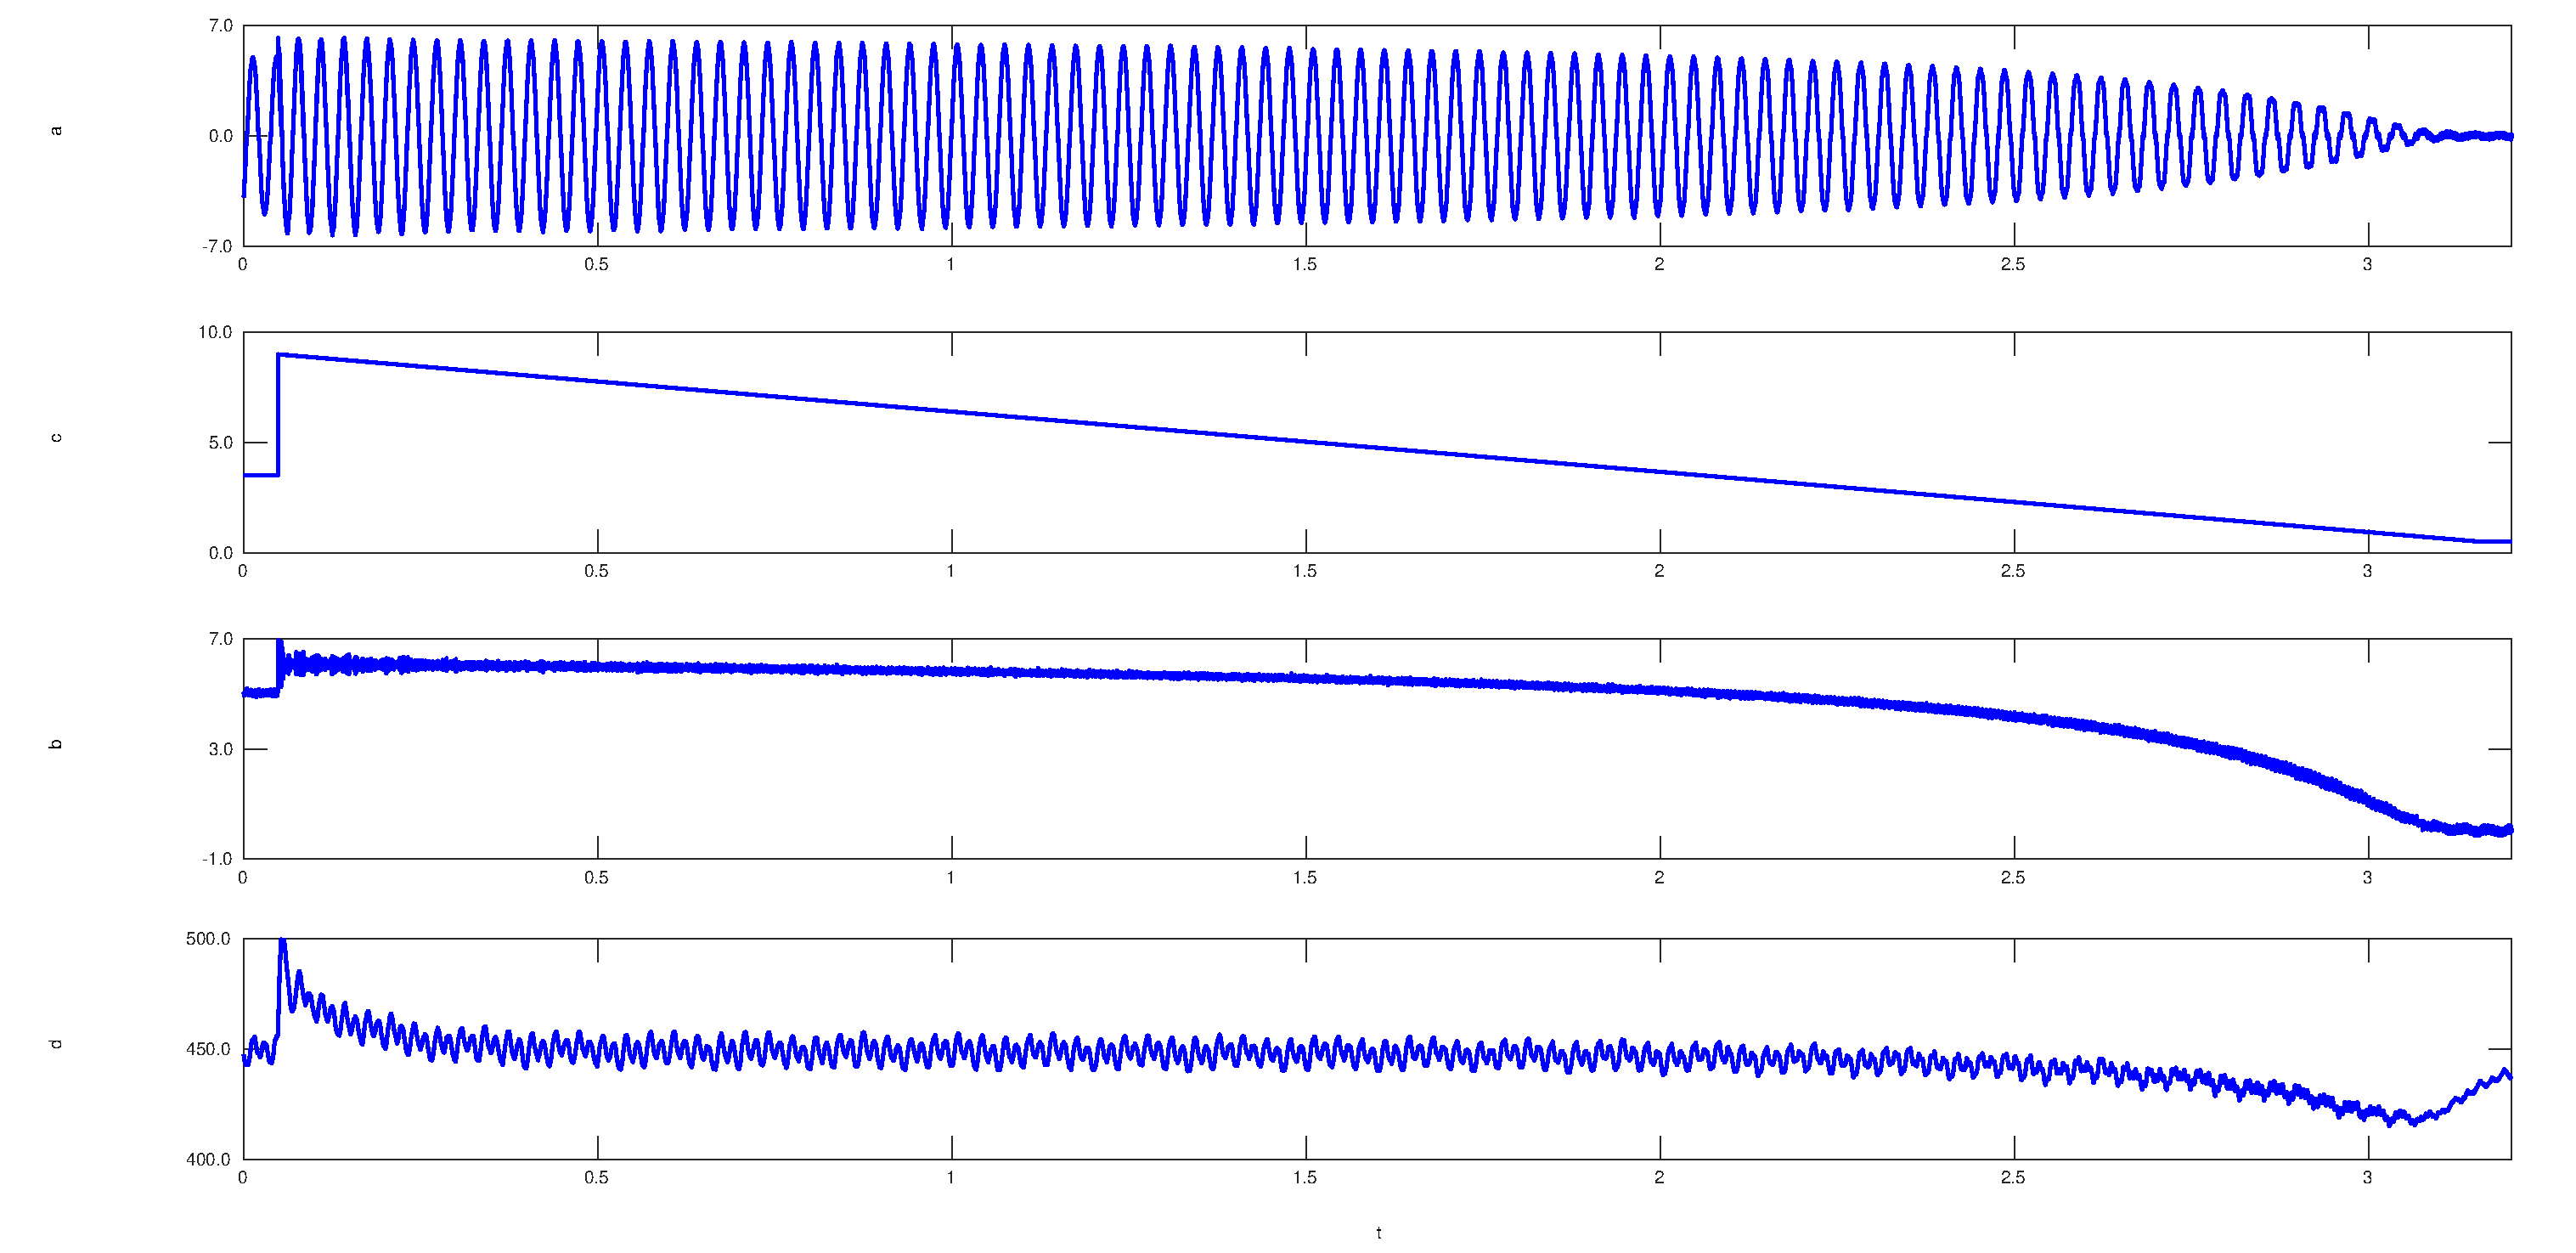
\includegraphics[width=0.50\textwidth]{./figures/L_robust_db.eps}\\
\caption{The steady-state performance under the stator inductance variation. (With the conventional CCS-MPCC, $\rm 450  \; rpm$, 5A $i_q$).}
\label{L_robust_db}
\end{figure}

\begin{figure}[htbp]
\def\size{0.6}
\def\sizetwo{0.45}
\centering
\psfrag{0}[tc][tc][\size]{$\bm{0}$}
\psfrag{0.5}[tc][tc][\size]{$\bm{0.5}$}
\psfrag{1}[tc][tc][\size]{$\bm{1}$}
\psfrag{1.5}[tc][tc][\size]{$\bm{1.5}$}
\psfrag{2}[tc][tc][\size]{$\bm{2}$}
\psfrag{2.5}[tc][tc][\size]{$\bm{2.5}$}
\psfrag{3}[tc][tc][\size]{$\bm{3}$}

\psfrag{0.0}[r][r][\size]{$\bm{0}$}
\psfrag{6.0}[r][r][\size]{$\bm{6}$}

\psfrag{4.0}[r][r][\size]{$\bm{4}$}
\psfrag{5.0}[r][r][\size]{$\bm{5}$}
\psfrag{-7.0}[r][r][\size]{$\bm{-7}$}
\psfrag{10.0}[r][r][\size]{$\bm{10}$}
\psfrag{-6.0}[r][r][\size]{$\bm{-6}$}
\psfrag{7.0}[r][r][\size]{$\bm{7}$}
\psfrag{-1.0}[r][r][\size]{$\bm{-1}$}
\psfrag{3.0}[r][r][\size]{$\bm{3}$}

\psfrag{500.0}[r][r][\size]{$\bm{500}$}
\psfrag{400.0}[r][r][\size]{$\bm{400}$}
\psfrag{450.0}[r][r][\size]{$\bm{450}$}


\psfrag{-1.00}[r][r][\size]{$\bm{-1}$}
\psfrag{0.00}[r][r][\sizetwo]{$\bm{0}$}
\psfrag{1.00}[r][r][\sizetwo]{$\bm{1}$}
\psfrag{0.500}[r][r][\sizetwo]{$\bm{0.5}$}
\psfrag{1.50}[r][r][\sizetwo]{$\bm{1.5}$}
\psfrag{2.00}[r][r][\sizetwo]{$\bm{2.0}$}
\psfrag{2.50}[r][r][\sizetwo]{$\bm{2.5}$}
\psfrag{3.00}[r][r][\sizetwo]{$\bm{3}$}
\psfrag{5.14}[r][r][\sizetwo]{$\bm{5.14}$}
\psfrag{4.86}[r][r][\sizetwo]{$\bm{4.86}$}
\psfrag{7.00}[r][r][\size]{$\bm{7}$}
\psfrag{3.50}[r][r][\size]{$\bm{3.5}$}


\psfrag{70}[r][r][\size]{$\bm{70}$}
\psfrag{80}[r][r][\size]{$\bm{80}$}
\psfrag{75}[r][r][\size]{$\bm{75}$}

\psfrag{t}[tc][tc][\size]{$\rm \textbf{Time  \; [s]}$}
\psfrag{d}[c][c][\size]{$\bm{\omega_m}  \; \rm \textbf{[rpm]}$}
\psfrag{b}[c][c][\size]{$\bm{i_q}  \; \rm \textbf {[A]}$}
\psfrag{a}[c][c][\size]{$\bm{i_a}  \; \rm \textbf {[A]}$}
\psfrag{c}[c][c][\size]{$\bm{i_d}  \; \rm \textbf {[A]}$}
\psfrag{c}[c][c][\size]{$\bm{L}  \; \rm \textbf  {[mH]}}$}
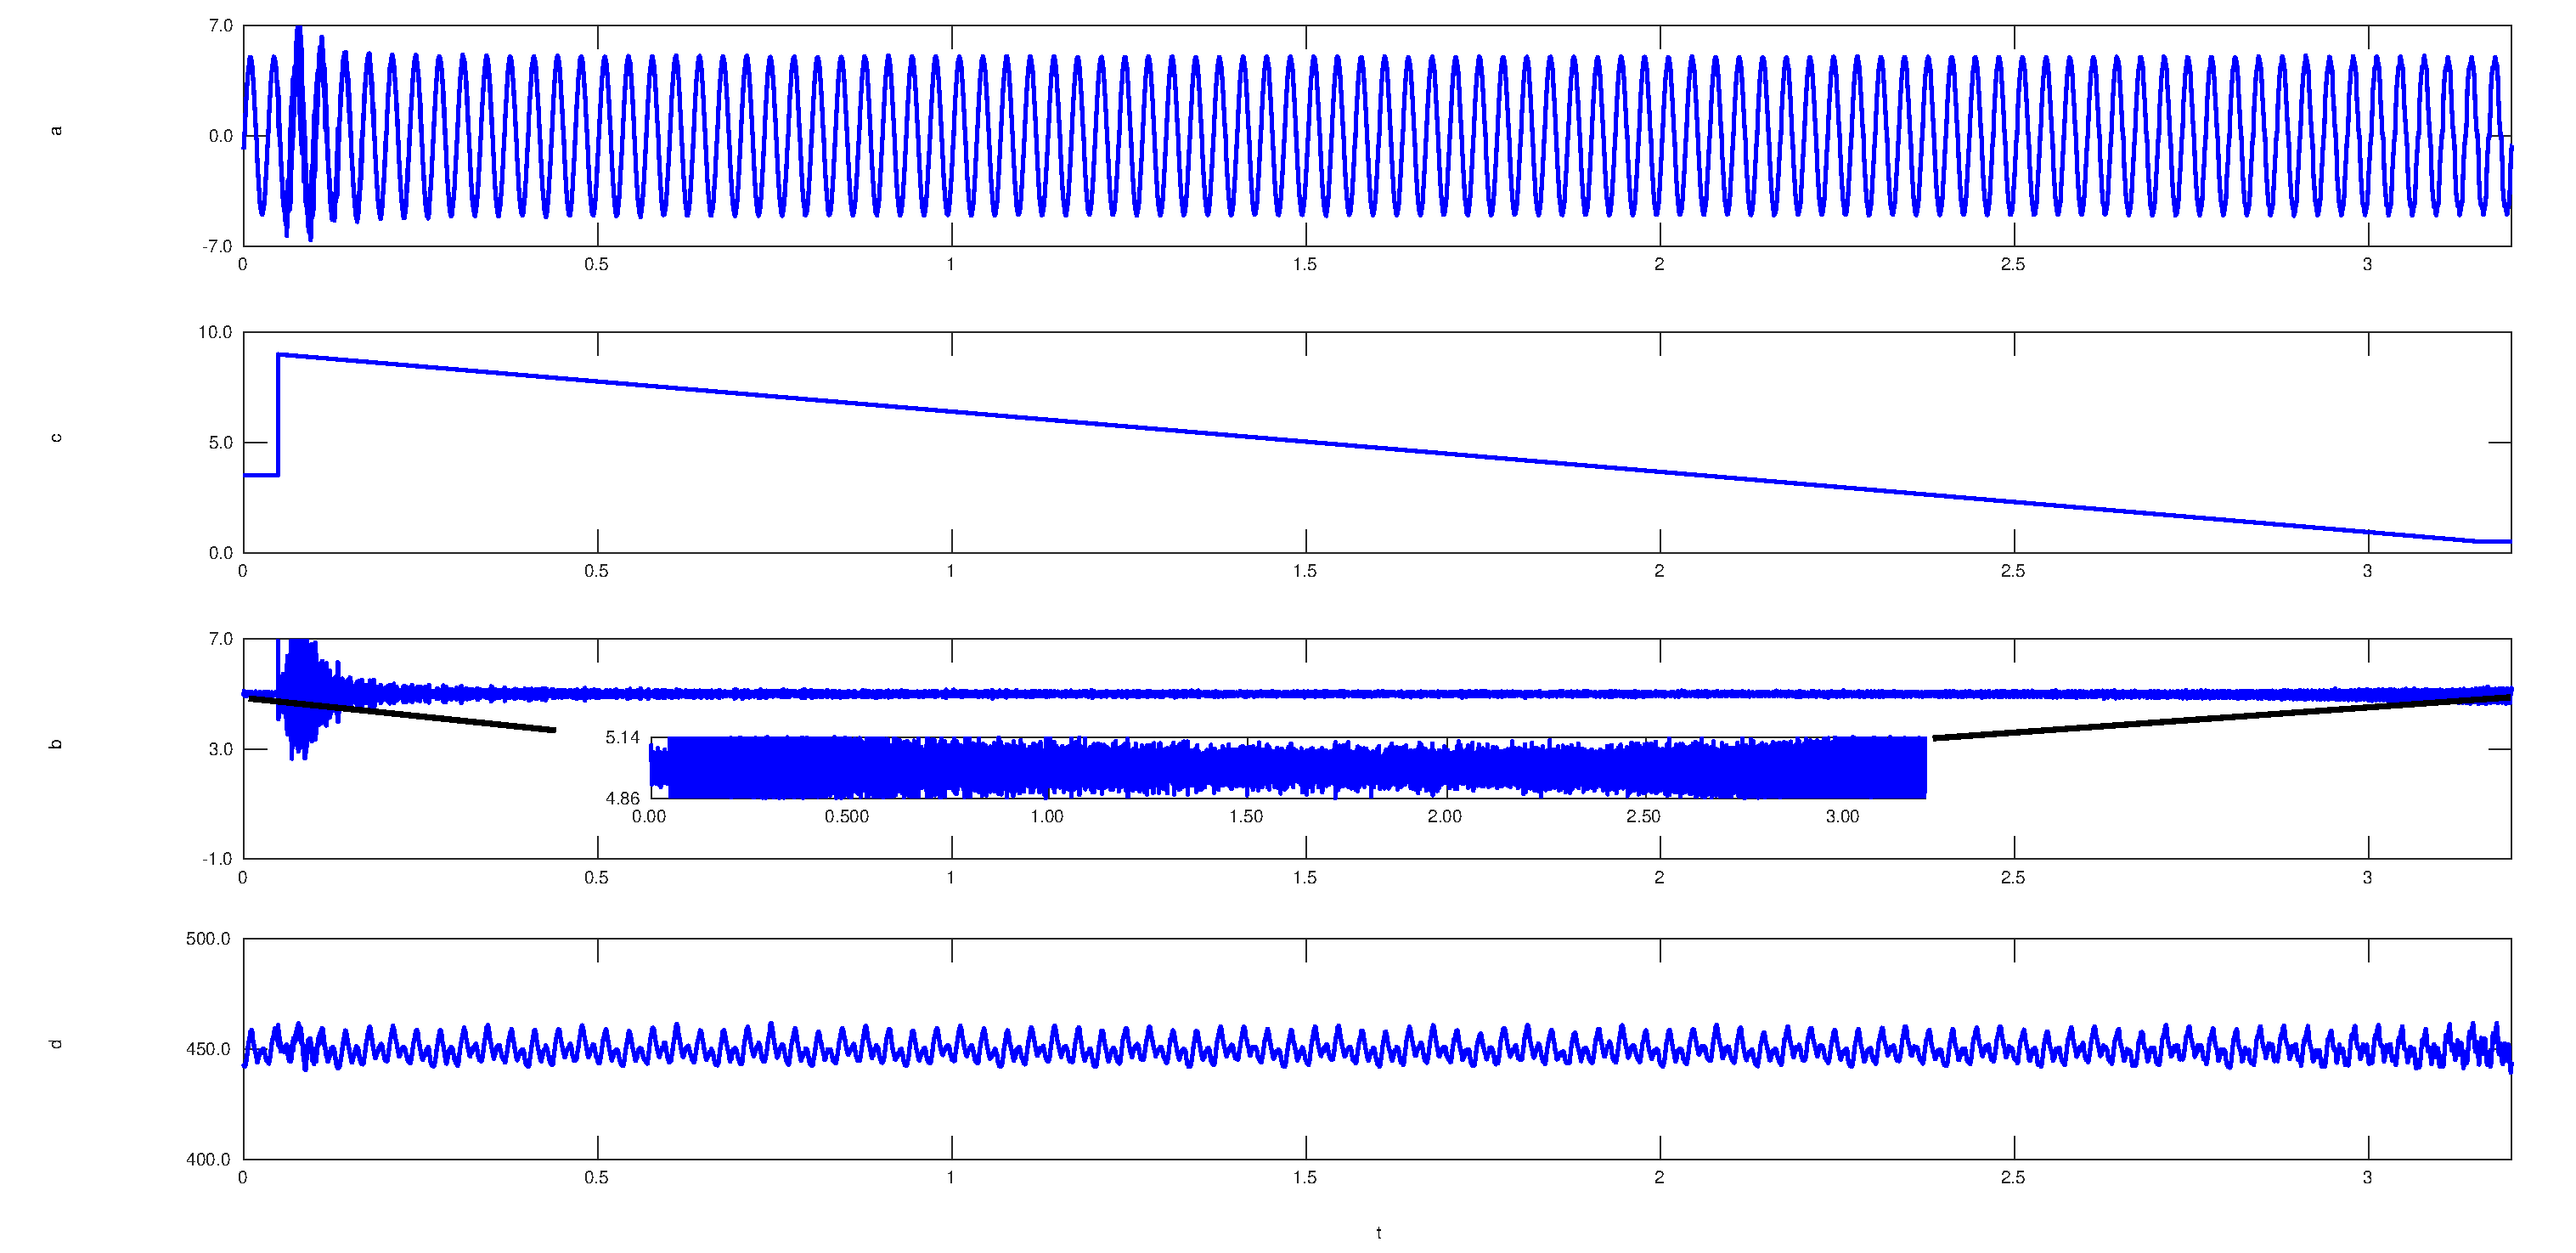
\includegraphics[width=0.50\textwidth]{./figures/L_robust_edb.eps}\\
\caption{The steady-state performance under the stator inductance variation. (With the EXM-CCSMPCC, $\rm 450  \; rpm$, 5A $i_q$).}
\label{L_robust_edb}
\end{figure}

\begin{figure}[htbp]
\def\size{0.6}
\def\sizetwo{0.45}
\centering
\psfrag{0}[tc][tc][\size]{$\bm{0}$}
\psfrag{0.5}[tc][tc][\size]{$\bm{0.5}$}
\psfrag{1}[tc][tc][\size]{$\bm{1}$}
\psfrag{1.5}[tc][tc][\size]{$\bm{1.5}$}
\psfrag{2}[tc][tc][\size]{$\bm{2}$}
\psfrag{2.5}[tc][tc][\size]{$\bm{2.5}$}
\psfrag{3}[tc][tc][\size]{$\bm{3}$}

\psfrag{0.0}[r][r][\size]{$\bm{0}$}
\psfrag{6.0}[r][r][\size]{$\bm{6}$}

\psfrag{4.0}[r][r][\size]{$\bm{4}$}
\psfrag{5.0}[r][r][\size]{$\bm{5}$}
\psfrag{-7.0}[r][r][\size]{$\bm{-7}$}
\psfrag{10.0}[r][r][\size]{$\bm{10}$}
\psfrag{-6.0}[r][r][\size]{$\bm{-6}$}
\psfrag{7.0}[r][r][\size]{$\bm{7}$}
\psfrag{-1.0}[r][r][\size]{$\bm{-1}$}
\psfrag{3.0}[r][r][\size]{$\bm{3}$}

\psfrag{500.0}[r][r][\size]{$\bm{500}$}
\psfrag{400.0}[r][r][\size]{$\bm{400}$}
\psfrag{450.0}[r][r][\size]{$\bm{450}$}


\psfrag{-1.00}[r][r][\size]{$\bm{-1}$}
\psfrag{0.00}[r][r][\sizetwo]{$\bm{0}$}
\psfrag{1.00}[r][r][\sizetwo]{$\bm{1}$}
\psfrag{0.500}[r][r][\sizetwo]{$\bm{0.5}$}
\psfrag{1.50}[r][r][\sizetwo]{$\bm{1.5}$}
\psfrag{2.00}[r][r][\sizetwo]{$\bm{2.0}$}
\psfrag{2.50}[r][r][\sizetwo]{$\bm{2.5}$}
\psfrag{3.00}[r][r][\sizetwo]{$\bm{3}$}
\psfrag{5.14}[r][r][\sizetwo]{$\bm{5.14}$}
\psfrag{4.86}[r][r][\sizetwo]{$\bm{4.86}$}
\psfrag{7.00}[r][r][\size]{$\bm{7}$}
\psfrag{3.50}[r][r][\size]{$\bm{3.5}$}


\psfrag{70}[r][r][\size]{$\bm{70}$}
\psfrag{80}[r][r][\size]{$\bm{80}$}
\psfrag{75}[r][r][\size]{$\bm{75}$}

\psfrag{t}[tc][tc][\size]{$\rm \textbf{Time  \; [s]}$}
\psfrag{d}[c][c][\size]{$\bm{\omega_m}  \; \rm \textbf{[rpm]}$}
\psfrag{b}[c][c][\size]{$\bm{i_q}  \; \rm \textbf {[A]}$}
\psfrag{a}[c][c][\size]{$\bm{i_a}  \; \rm \textbf {[A]}$}
\psfrag{c}[c][c][\size]{$\bm{i_d}  \; \rm \textbf {[A]}$}
\psfrag{c}[c][c][\size]{$\bm{L}  \; \rm \textbf  {[mH]}}$}
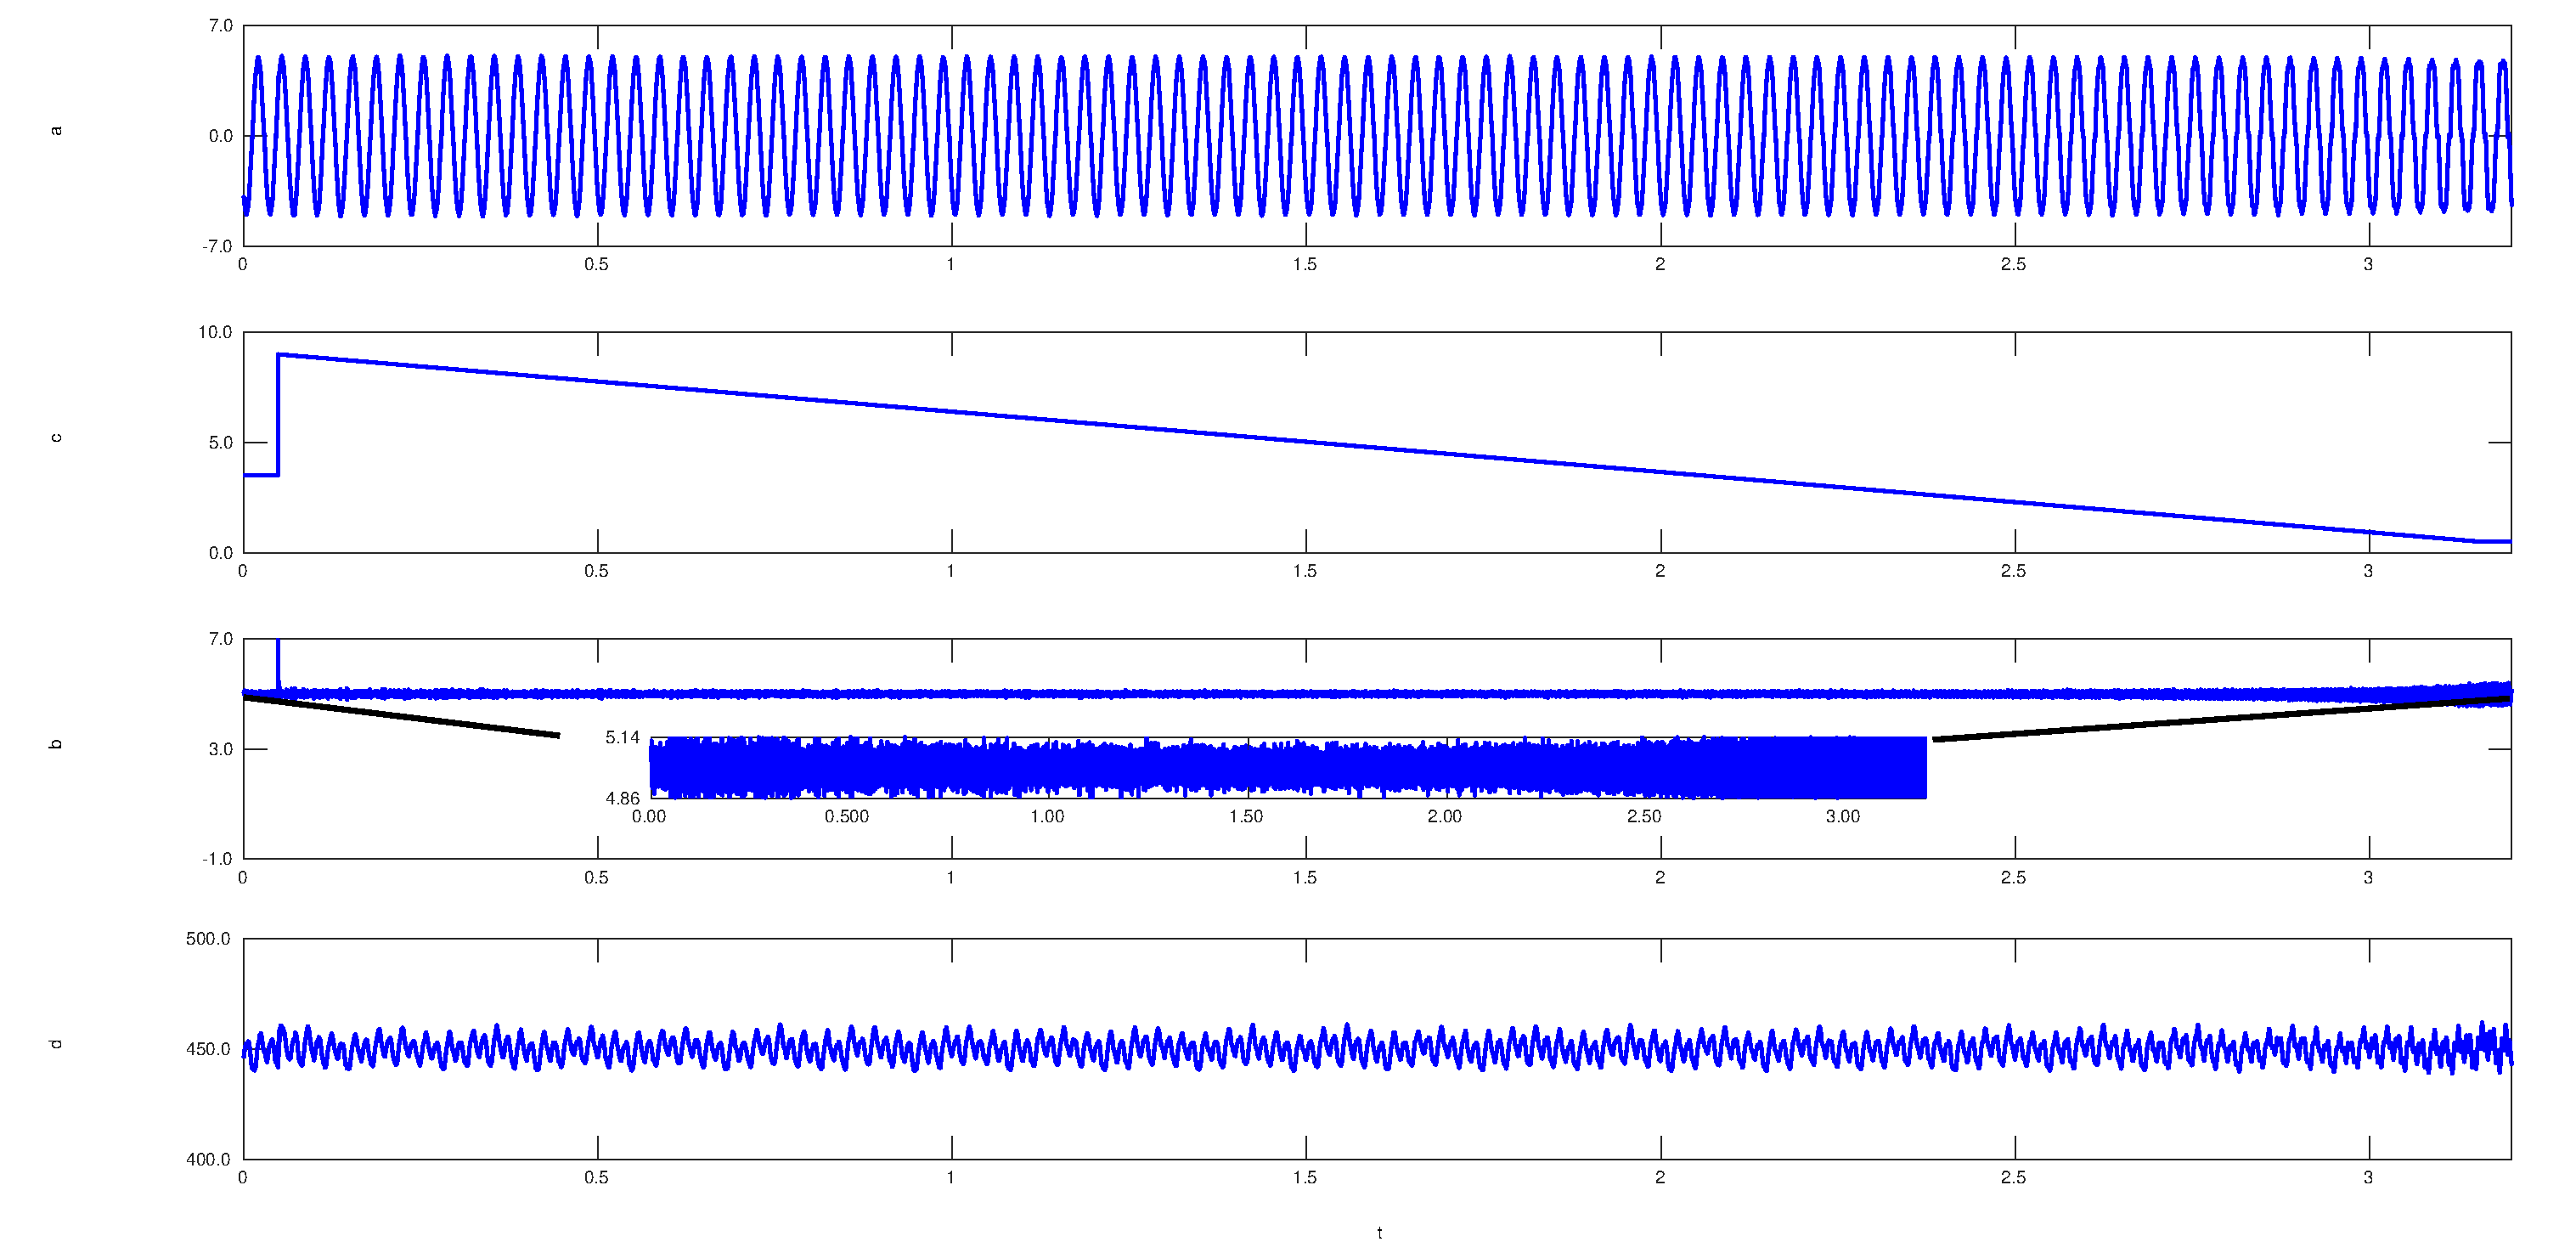
\includegraphics[width=0.50\textwidth]{./figures/L_robust_et.eps}\\
\caption{The steady-state performance under the stator inductance variation. (With the MSET-CCSMPCC, $\rm 450  \; rpm$, 5A $i_q$).}
\label{L_robust_et}
\end{figure}

\section{Conclusion}
This paper has proposed a robust continuous control set model-based predictive current control method for an SPMSM. An extended SPMSM model and a fast terminal sliding mode disturbance observer are considered for disturbance compensation. Furthermore, a multi-step error tracking CCS-MPCC is proposed to reduce the overshoot while keeping excellent steady-state and dynamic response performances. The experimental results implemented on an FPGA-based hardware verify the effectiveness of the proposed methods. The further work is to improve the algorithm robustness in a wider range of inductance variations.
\iffalse
This paper has proposed an EXM-CCSMPCC and an MSET-CCSMPCC. The contributions of the paper include
			\begin{itemize}
			\item An FTSMDO with a SMD is designed to estimate the disturbance of the extended SPMSM model.
			\item An extended SPMSM model based EXM-CCSMPCC is proposed to improve the robustness against lumped disturbances. 
			\item An MSET-CCSMPCC is proposed to reduce the overshoot while keeping good steady-state and dynamic response performances.  
			\end{itemize}
\fi

\iffalse
Conventionally, CCS-MPCC has excellent dynamic performance and good steady-state performance. However, the performance of conventional CCS-MPCC depends heavily on the motor parameters, the variations of which usually cause steady-state errors. To solve the problem, EXM-CCSMPCC which is based on the extended SPMSM model is proposed. By introducing an FTSMDO, the lumped disturbance of the extended SPMSM model is estimated and used as a feedforward to compensate the CCS-MPCC controller. AS the $i_d$ and $i_q$ track the $i_d^*$ and $i_q^*$ as fast as possible, there is overshoot in the step performance test with EXM-CCSMPCC. To eliminate the overshoot, MSET-CCSMPCC is proposed.
Experiments were carried out, whose results show that compared with conventional CCS-MPCC, the proposed EXM-CCSMPCC and MSET-CCSMPCC methods not only eliminate the steady-state errors, but also exhibit better dynamic performance, better steady-state performance and more robust to motor parameters. 
Experiments show that the designed FTSMDO reduces the chattering level on the estimated d- and q- axes stator currents and disturbances while maintaining fast tracking performance, and the proposed EXM-CCSMPCC and MSET-CCSMPCC have good dynamic response and steady-state performances, and the MSET-CCSMPCC further suppresses the overshoot in the step response test.
\fi


%\section*{ACKNOWLEDGEMENTS}


\bibliographystyle{IEEEtran}
\bibliography{IEEEabrv,References}
\vspace{-8ex}
% biography section

\iffalse 
\begin{IEEEbiography}[{\includegraphics[width=1in,height=1.25in,clip,keepaspectratio]{./Authorphotographs/Wang1.eps}}]{Fengxiang Wang}

was born in Jiujiang, China, in 1982. He received the B.S. degree in electronic engineering and the M.S. degree in automation from Nanchang Hangkong University, Nanchang, China, in 2005 and 2008, respectively. In 2014, he was awarded Ph.D. degree in electrical engineering at the Institute for Electrical Drive Systems and Power Electronics, Technische Universitaet Muenchen, Munich, Germany. Since Sep. 2014 he works as a professor in Quanzhou Institute of Equipment Manufacturing, Haixi Institutes, Chinese Academy of Sciences.

His research interests include predictive control and sensorless control for electrical drives.
\vspace{-12ex}
\end{IEEEbiography}


\begin{IEEEbiography}[{\includegraphics[width=1in,height=1.25in,clip,keepaspectratio]{./Authorphotographs/kennel7.eps}}]{Ralph Kennel }
was born in 1955 at Kaiserslautern (Germany). In 1979 he got his diploma degree and in 1984 his Dr.-Ing. (Ph.D.) degree from the University of Kaiserslautern.

From 1983 to 1999 he worked on several positions with Robert BOSCH GmbH (Germany). Until 1997 he was responsible for the development of servo drives. 
From 1994 to 1999 Dr. Kennel was appointed Visiting Professor at the University of Newcastle-upon-Tyne (England, UK). From 1999 - 2008 he was Professor for Electrical Machines and Drives at Wuppertal University (Germany). Since 2008 he is Professor for Electrical Drive systems and Power Electronics at Technische Universtaet Muenchen (Germany). His main interests today are: Sensorless control of AC drives, predictive control of power electronics and Hardware-in-the-Loop systems.

Dr. Kennel is a Senior Member of IEEE, a Fellow of IEE and a Chartered Engineer in the UK. Within IEEE he is Treasurer of the Germany Section as well as ECCE Global Partnership Chair of the Power Electronics society (PELS).
\vspace{-8ex}
\end{IEEEbiography}



\begin{IEEEbiography}[{\includegraphics[width=1in,height=1.25in,clip,keepaspectratio]{./Authorphotographs/Rodriguez6.eps}}]{Jos\'{e}~Rodr\'{i}guez }
(M'81-SM'94-F10)   Received the Engineer degree in electrical engineering from the Universidad Federico Santa Maria (UTFSM), Valparaiso, Chile, in 1977 and the Dr.-Ing. degree in electrical engineering from the University of Erlangen, Erlangen, Germany, in 1985.

He had been with the Department of Electronics Engineering, University Federico Santa Maria since 1977, where he was full Professor and Rector. Since 2014, he has been with Universidad Andres Bello, where he is currently Rector.

He has co-authored more than 300 journal and conference papers. His main research interests include multilevel inverters, new converter topologies, control of power converters, and adjustable-speed drives.

Prof. Rodriguez is Associate Editor of the IEEE TRANSACTIONS ON POWER ELECTRONICS and IEEE TRANSACTIONS ON INDUSTRIAL ELECTRONICS since 2002. He received the Best Paper Award from the IEEE INDUSTRIAL ELECTRONICS MAGAZINE in 2008, Best Paper Award from the IEEE TRANSACTIONS ON POWER ELECTRONICS in 2010 and the Best Paper Award from the IEEE TRANSACTIONS ON INDUSTRIAL ELECTRONICS in 2007 and 2011.
Dr. Rodríguez is member of the Chilean Academy of Engineering and Fellow of the IEEE.  
\vspace{-8ex}
\end{IEEEbiography}
\fi


\end{document}
